\documentclass[twoside]{book}

% Packages required by doxygen
\usepackage{fixltx2e}
\usepackage{calc}
\usepackage{doxygen}
\usepackage[export]{adjustbox} % also loads graphicx
\usepackage{graphicx}
\usepackage[utf8]{inputenc}
\usepackage{makeidx}
\usepackage{multicol}
\usepackage{multirow}
\PassOptionsToPackage{warn}{textcomp}
\usepackage{textcomp}
\usepackage[nointegrals]{wasysym}
\usepackage[table]{xcolor}

% Font selection
\usepackage[T1]{fontenc}
\usepackage[scaled=.90]{helvet}
\usepackage{courier}
\usepackage{amssymb}
\usepackage{sectsty}
\renewcommand{\familydefault}{\sfdefault}
\allsectionsfont{%
  \fontseries{bc}\selectfont%
  \color{darkgray}%
}
\renewcommand{\DoxyLabelFont}{%
  \fontseries{bc}\selectfont%
  \color{darkgray}%
}
\newcommand{\+}{\discretionary{\mbox{\scriptsize$\hookleftarrow$}}{}{}}

% Page & text layout
\usepackage{geometry}
\geometry{%
  a4paper,%
  top=2.5cm,%
  bottom=2.5cm,%
  left=2.5cm,%
  right=2.5cm%
}
\tolerance=750
\hfuzz=15pt
\hbadness=750
\setlength{\emergencystretch}{15pt}
\setlength{\parindent}{0cm}
\setlength{\parskip}{0.2cm}
\makeatletter
\renewcommand{\paragraph}{%
  \@startsection{paragraph}{4}{0ex}{-1.0ex}{1.0ex}{%
    \normalfont\normalsize\bfseries\SS@parafont%
  }%
}
\renewcommand{\subparagraph}{%
  \@startsection{subparagraph}{5}{0ex}{-1.0ex}{1.0ex}{%
    \normalfont\normalsize\bfseries\SS@subparafont%
  }%
}
\makeatother

% Headers & footers
\usepackage{fancyhdr}
\pagestyle{fancyplain}
\fancyhead[LE]{\fancyplain{}{\bfseries\thepage}}
\fancyhead[CE]{\fancyplain{}{}}
\fancyhead[RE]{\fancyplain{}{\bfseries\leftmark}}
\fancyhead[LO]{\fancyplain{}{\bfseries\rightmark}}
\fancyhead[CO]{\fancyplain{}{}}
\fancyhead[RO]{\fancyplain{}{\bfseries\thepage}}
\fancyfoot[LE]{\fancyplain{}{}}
\fancyfoot[CE]{\fancyplain{}{}}
\fancyfoot[RE]{\fancyplain{}{\bfseries\scriptsize Generated on Sun Jun 14 2015 20\+:59\+:16 for L\+O21 $\vert$ Pistache by Doxygen }}
\fancyfoot[LO]{\fancyplain{}{\bfseries\scriptsize Generated on Sun Jun 14 2015 20\+:59\+:16 for L\+O21 $\vert$ Pistache by Doxygen }}
\fancyfoot[CO]{\fancyplain{}{}}
\fancyfoot[RO]{\fancyplain{}{}}
\renewcommand{\footrulewidth}{0.4pt}
\renewcommand{\chaptermark}[1]{%
  \markboth{#1}{}%
}
\renewcommand{\sectionmark}[1]{%
  \markright{\thesection\ #1}%
}

% Indices & bibliography
\usepackage{natbib}
\usepackage[titles]{tocloft}
\setcounter{tocdepth}{3}
\setcounter{secnumdepth}{5}
\makeindex

% Hyperlinks (required, but should be loaded last)
\usepackage{ifpdf}
\ifpdf
  \usepackage[pdftex,pagebackref=true]{hyperref}
\else
  \usepackage[ps2pdf,pagebackref=true]{hyperref}
\fi
\hypersetup{%
  colorlinks=true,%
  linkcolor=blue,%
  citecolor=blue,%
  unicode%
}

% Custom commands
\newcommand{\clearemptydoublepage}{%
  \newpage{\pagestyle{empty}\cleardoublepage}%
}


%===== C O N T E N T S =====

\begin{document}

% Titlepage & ToC
\hypersetup{pageanchor=false,
             bookmarks=true,
             bookmarksnumbered=true,
             pdfencoding=unicode
            }
\pagenumbering{roman}
\begin{titlepage}
\vspace*{7cm}
\begin{center}%
{\Large L\+O21 $\vert$ Pistache }\\
\vspace*{1cm}
{\large Generated by Doxygen 1.8.9.1}\\
\vspace*{0.5cm}
{\small Sun Jun 14 2015 20:59:16}\\
\end{center}
\end{titlepage}
\clearemptydoublepage
\tableofcontents
\clearemptydoublepage
\pagenumbering{arabic}
\hypersetup{pageanchor=true}

%--- Begin generated contents ---
\chapter{Namespace Index}
\section{Namespace List}
Here is a list of all namespaces with brief descriptions\+:\begin{DoxyCompactList}
\item\contentsline{section}{\hyperlink{namespace_t_i_m_e}{T\+I\+M\+E} }{\pageref{namespace_t_i_m_e}}{}
\item\contentsline{section}{\hyperlink{namespace_ui}{Ui} }{\pageref{namespace_ui}}{}
\end{DoxyCompactList}

\chapter{Hierarchical Index}
\section{Class Hierarchy}
This inheritance list is sorted roughly, but not completely, alphabetically\+:\begin{DoxyCompactList}
\item \contentsline{section}{Activite}{\pageref{class_activite}}{}
\item \contentsline{section}{Calendar\+Exception}{\pageref{class_calendar_exception}}{}
\item \contentsline{section}{T\+I\+M\+E\+:\+:Date}{\pageref{class_t_i_m_e_1_1_date}}{}
\item \contentsline{section}{T\+I\+M\+E\+:\+:Duree}{\pageref{class_t_i_m_e_1_1_duree}}{}
\item \contentsline{section}{T\+I\+M\+E\+:\+:Horaire}{\pageref{class_t_i_m_e_1_1_horaire}}{}
\item \contentsline{section}{T\+I\+M\+E\+:\+:Intervalle}{\pageref{class_t_i_m_e_1_1_intervalle}}{}
\item \contentsline{section}{Tache\+:\+:Iterator}{\pageref{class_tache_1_1_iterator}}{}
\item \contentsline{section}{Projet\+:\+:Iterator}{\pageref{class_projet_1_1_iterator}}{}
\item \contentsline{section}{Composite\+:\+:iterator}{\pageref{class_composite_1_1iterator}}{}
\item \contentsline{section}{T\+I\+M\+E\+:\+:Periode}{\pageref{class_t_i_m_e_1_1_periode}}{}
\item \contentsline{section}{Programmation}{\pageref{class_programmation}}{}
\item \contentsline{section}{Programmation\+Manager}{\pageref{class_programmation_manager}}{}
\item \contentsline{section}{Projet}{\pageref{class_projet}}{}
\item Q\+Main\+Window\begin{DoxyCompactList}
\item \contentsline{section}{Main\+Window}{\pageref{class_main_window}}{}
\end{DoxyCompactList}
\item \contentsline{section}{T\+I\+M\+E\+:\+:Time\+Exception}{\pageref{class_t_i_m_e_1_1_time_exception}}{}
\item \contentsline{section}{Truc}{\pageref{class_truc}}{}
\begin{DoxyCompactList}
\item \contentsline{section}{Tache}{\pageref{class_tache}}{}
\begin{DoxyCompactList}
\item \contentsline{section}{Composite}{\pageref{class_composite}}{}
\item \contentsline{section}{Unitaire}{\pageref{class_unitaire}}{}
\end{DoxyCompactList}
\end{DoxyCompactList}
\end{DoxyCompactList}

\chapter{Class Index}
\section{Class List}
Here are the classes, structs, unions and interfaces with brief descriptions\+:\begin{DoxyCompactList}
\item\contentsline{section}{\hyperlink{class_activite}{Activite} }{\pageref{class_activite}}{}
\item\contentsline{section}{\hyperlink{class_calendar_exception}{Calendar\+Exception} \\*Classe d\textquotesingle{}affichage des erreurs }{\pageref{class_calendar_exception}}{}
\item\contentsline{section}{\hyperlink{class_composite}{Composite} \\*\hyperlink{class_tache}{Tache} qui peut contenir des tâches mais ne peut pas être programmée }{\pageref{class_composite}}{}
\item\contentsline{section}{\hyperlink{class_t_i_m_e_1_1_date}{T\+I\+M\+E\+::\+Date} \\*Classe permettant de manipuler des dates standards L\textquotesingle{}utilisation de cette classe n�cessite des dates valides au sens commun du terme. D�clenchement d\textquotesingle{}exception dans le cas contraire }{\pageref{class_t_i_m_e_1_1_date}}{}
\item\contentsline{section}{\hyperlink{class_t_i_m_e_1_1_duree}{T\+I\+M\+E\+::\+Duree} \\*Classe permettant de manipuler des durees L\textquotesingle{}utilisation de cette classe n�cessite des dates valides au sens commun du terme. D�clenchement d\textquotesingle{}exception dans le cas contraire }{\pageref{class_t_i_m_e_1_1_duree}}{}
\item\contentsline{section}{\hyperlink{class_t_i_m_e_1_1_horaire}{T\+I\+M\+E\+::\+Horaire} \\*Classe permettant de manipuler des horaires L\textquotesingle{}utilisation de cette classe n�cessite des dates valides au sens commun du terme. D�clenchement d\textquotesingle{}exception dans le cas contraire }{\pageref{class_t_i_m_e_1_1_horaire}}{}
\item\contentsline{section}{\hyperlink{class_t_i_m_e_1_1_intervalle}{T\+I\+M\+E\+::\+Intervalle} \\*Classe permettant de manipuler des intervalles de dates L\textquotesingle{}utilisation de cette classe n�cessite des dates valides au sens commun du terme. D�clenchement d\textquotesingle{}exception dans le cas contraire }{\pageref{class_t_i_m_e_1_1_intervalle}}{}
\item\contentsline{section}{\hyperlink{class_tache_1_1_iterator}{Tache\+::\+Iterator} }{\pageref{class_tache_1_1_iterator}}{}
\item\contentsline{section}{\hyperlink{class_projet_1_1_iterator}{Projet\+::\+Iterator} }{\pageref{class_projet_1_1_iterator}}{}
\item\contentsline{section}{\hyperlink{class_composite_1_1iterator}{Composite\+::iterator} }{\pageref{class_composite_1_1iterator}}{}
\item\contentsline{section}{\hyperlink{class_main_window}{Main\+Window} \\*Conserve les pointeurs vers les principaux widgets de la fenêtre. S\textquotesingle{}occupe des actions générales sur ceux-\/ci }{\pageref{class_main_window}}{}
\item\contentsline{section}{\hyperlink{class_t_i_m_e_1_1_periode}{T\+I\+M\+E\+::\+Periode} \\*Classe permettant de manipuler des periodes exprim�es en jours/mois/ann�es L\textquotesingle{}utilisation de cette classe n�cessite des dates valides au sens commun du terme. D�clenchement d\textquotesingle{}exception dans le cas contraire }{\pageref{class_t_i_m_e_1_1_periode}}{}
\item\contentsline{section}{\hyperlink{class_programmation}{Programmation} }{\pageref{class_programmation}}{}
\item\contentsline{section}{\hyperlink{class_programmation_manager}{Programmation\+Manager} \\*Gestion des évènements ou taches programmés }{\pageref{class_programmation_manager}}{}
\item\contentsline{section}{\hyperlink{class_projet}{Projet} \\*Un ensemble de tache à réaliser }{\pageref{class_projet}}{}
\item\contentsline{section}{\hyperlink{class_tache}{Tache} \\*Classe abstraite mère de toutes les taches. Comporte un titre, une échéance et une liste de précédences (taches à réaliser avant de pouvoir à commencer celle-\/ci) }{\pageref{class_tache}}{}
\item\contentsline{section}{\hyperlink{class_t_i_m_e_1_1_time_exception}{T\+I\+M\+E\+::\+Time\+Exception} \\*Classe permettant de g�rer les exceptions des classes du namespace T\+I\+M\+E }{\pageref{class_t_i_m_e_1_1_time_exception}}{}
\item\contentsline{section}{\hyperlink{class_truc}{Truc} }{\pageref{class_truc}}{}
\item\contentsline{section}{\hyperlink{class_unitaire}{Unitaire} \\*\hyperlink{class_tache}{Tache} programmable }{\pageref{class_unitaire}}{}
\end{DoxyCompactList}

\chapter{File Index}
\section{File List}
Here is a list of all files with brief descriptions\+:\begin{DoxyCompactList}
\item\contentsline{section}{L\+O21app/\hyperlink{agendaview_8cpp}{agendaview.\+cpp} }{\pageref{agendaview_8cpp}}{}
\item\contentsline{section}{L\+O21app/\hyperlink{agendaview_8h}{agendaview.\+h} }{\pageref{agendaview_8h}}{}
\item\contentsline{section}{L\+O21app/\hyperlink{_calendar_8cpp}{Calendar.\+cpp} }{\pageref{_calendar_8cpp}}{}
\item\contentsline{section}{L\+O21app/\hyperlink{_calendar_8h}{Calendar.\+h} }{\pageref{_calendar_8h}}{}
\item\contentsline{section}{L\+O21app/\hyperlink{eventwidget_8cpp}{eventwidget.\+cpp} }{\pageref{eventwidget_8cpp}}{}
\item\contentsline{section}{L\+O21app/\hyperlink{eventwidget_8h}{eventwidget.\+h} }{\pageref{eventwidget_8h}}{}
\item\contentsline{section}{L\+O21app/\hyperlink{main_8cpp}{main.\+cpp} }{\pageref{main_8cpp}}{}
\item\contentsline{section}{L\+O21app/\hyperlink{_main_window_8cpp}{Main\+Window.\+cpp} }{\pageref{_main_window_8cpp}}{}
\item\contentsline{section}{L\+O21app/\hyperlink{_main_window_8h}{Main\+Window.\+h} }{\pageref{_main_window_8h}}{}
\item\contentsline{section}{L\+O21app/\hyperlink{timing_8cpp}{timing.\+cpp} }{\pageref{timing_8cpp}}{}
\item\contentsline{section}{L\+O21app/\hyperlink{timing_8h}{timing.\+h} }{\pageref{timing_8h}}{}
\item\contentsline{section}{L\+O21app/\hyperlink{_u_i_classes_8cpp}{U\+I\+Classes.\+cpp} }{\pageref{_u_i_classes_8cpp}}{}
\item\contentsline{section}{L\+O21app/\hyperlink{_u_i_classes_8h}{U\+I\+Classes.\+h} }{\pageref{_u_i_classes_8h}}{}
\end{DoxyCompactList}

\chapter{Namespace Documentation}
\hypertarget{namespace_t_i_m_e}{}\section{T\+I\+M\+E Namespace Reference}
\label{namespace_t_i_m_e}\index{T\+I\+M\+E@{T\+I\+M\+E}}
\subsection*{Classes}
\begin{DoxyCompactItemize}
\item 
class \hyperlink{class_t_i_m_e_1_1_date}{Date}
\begin{DoxyCompactList}\small\item\em Classe permettant de manipuler des dates standards L\textquotesingle{}utilisation de cette classe n�cessite des dates valides au sens commun du terme. D�clenchement d\textquotesingle{}exception dans le cas contraire. \end{DoxyCompactList}\item 
class \hyperlink{class_t_i_m_e_1_1_duree}{Duree}
\begin{DoxyCompactList}\small\item\em Classe permettant de manipuler des durees L\textquotesingle{}utilisation de cette classe n�cessite des dates valides au sens commun du terme. D�clenchement d\textquotesingle{}exception dans le cas contraire. \end{DoxyCompactList}\item 
class \hyperlink{class_t_i_m_e_1_1_horaire}{Horaire}
\begin{DoxyCompactList}\small\item\em Classe permettant de manipuler des horaires L\textquotesingle{}utilisation de cette classe n�cessite des dates valides au sens commun du terme. D�clenchement d\textquotesingle{}exception dans le cas contraire. \end{DoxyCompactList}\item 
class \hyperlink{class_t_i_m_e_1_1_intervalle}{Intervalle}
\begin{DoxyCompactList}\small\item\em Classe permettant de manipuler des intervalles de dates L\textquotesingle{}utilisation de cette classe n�cessite des dates valides au sens commun du terme. D�clenchement d\textquotesingle{}exception dans le cas contraire. \end{DoxyCompactList}\item 
class \hyperlink{class_t_i_m_e_1_1_periode}{Periode}
\begin{DoxyCompactList}\small\item\em Classe permettant de manipuler des periodes exprim�es en jours/mois/ann�es L\textquotesingle{}utilisation de cette classe n�cessite des dates valides au sens commun du terme. D�clenchement d\textquotesingle{}exception dans le cas contraire. \end{DoxyCompactList}\item 
class \hyperlink{class_t_i_m_e_1_1_time_exception}{Time\+Exception}
\begin{DoxyCompactList}\small\item\em Classe permettant de g�rer les exceptions des classes du namespace \hyperlink{namespace_t_i_m_e}{T\+I\+M\+E}. \end{DoxyCompactList}\end{DoxyCompactItemize}

\hypertarget{namespace_ui}{}\section{Ui Namespace Reference}
\label{namespace_ui}\index{Ui@{Ui}}

\chapter{Class Documentation}
\hypertarget{class_activite}{}\section{Activite Class Reference}
\label{class_activite}\index{Activite@{Activite}}


Classe d\textquotesingle{}evenement basique programmable, héritant d\textquotesingle{}\hyperlink{class_evenement}{Evenement} La classe possède un titre et un lieu.  




{\ttfamily \#include $<$Calendar.\+h$>$}



Inheritance diagram for Activite\+:\nopagebreak
\begin{figure}[H]
\begin{center}
\leavevmode
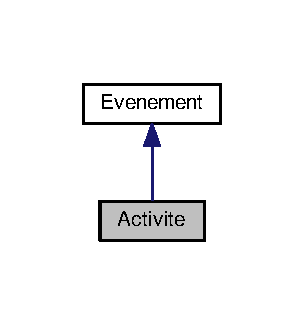
\includegraphics[width=146pt]{class_activite__inherit__graph}
\end{center}
\end{figure}


Collaboration diagram for Activite\+:\nopagebreak
\begin{figure}[H]
\begin{center}
\leavevmode
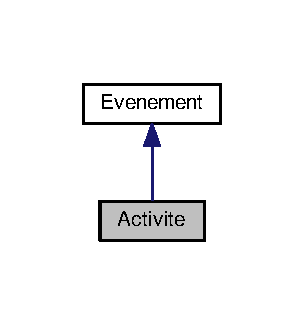
\includegraphics[width=146pt]{class_activite__coll__graph}
\end{center}
\end{figure}
\subsection*{Public Member Functions}
\begin{DoxyCompactItemize}
\item 
\hyperlink{class_activite_a06098c0f62244f4b60d250325b738094}{Activite} (const string \&t, const string \&l, \hyperlink{class_t_i_m_e_1_1_duree}{Duree} dur)
\begin{DoxyCompactList}\small\item\em Constructeur d\textquotesingle{}activité \end{DoxyCompactList}\item 
string \hyperlink{class_activite_ab0e1e83e41d35906dffc14530826075e}{get\+Titre} () const 
\begin{DoxyCompactList}\small\item\em Retourne le titre. \end{DoxyCompactList}\item 
string \hyperlink{class_activite_a695b4d43546d5715977381a7070d66d6}{get\+Lieu} () const 
\begin{DoxyCompactList}\small\item\em Retourne le lieu. \end{DoxyCompactList}\item 
void \hyperlink{class_activite_a510383c92c6d87877e074032fa8519ee}{set\+Titre} (const string \&t)
\begin{DoxyCompactList}\small\item\em Modifie le titre. \end{DoxyCompactList}\item 
void \hyperlink{class_activite_a1240cc984d5508b99feb99175bc05750}{set\+Lieu} (const string \&l)
\begin{DoxyCompactList}\small\item\em Modifie le lieu. \end{DoxyCompactList}\item 
void \hyperlink{class_activite_a513d49fbf721923d0db22a646ec606be}{update} (string t, string l, \hyperlink{class_t_i_m_e_1_1_duree}{Duree} d)
\item 
virtual void \hyperlink{class_activite_acf748b87edc5e4a5b78bd5e9364946f3}{afficher} (ostream \&f)
\begin{DoxyCompactList}\small\item\em Affiche les attributs de l\textquotesingle{}activité \end{DoxyCompactList}\end{DoxyCompactItemize}


\subsection{Detailed Description}
Classe d\textquotesingle{}evenement basique programmable, héritant d\textquotesingle{}\hyperlink{class_evenement}{Evenement} La classe possède un titre et un lieu. 

\subsection{Constructor \& Destructor Documentation}
\hypertarget{class_activite_a06098c0f62244f4b60d250325b738094}{}\index{Activite@{Activite}!Activite@{Activite}}
\index{Activite@{Activite}!Activite@{Activite}}
\subsubsection[{Activite}]{\setlength{\rightskip}{0pt plus 5cm}Activite\+::\+Activite (
\begin{DoxyParamCaption}
\item[{const string \&}]{t, }
\item[{const string \&}]{l, }
\item[{{\bf Duree}}]{dur}
\end{DoxyParamCaption}
)\hspace{0.3cm}{\ttfamily [inline]}}\label{class_activite_a06098c0f62244f4b60d250325b738094}


Constructeur d\textquotesingle{}activité 



\subsection{Member Function Documentation}
\hypertarget{class_activite_acf748b87edc5e4a5b78bd5e9364946f3}{}\index{Activite@{Activite}!afficher@{afficher}}
\index{afficher@{afficher}!Activite@{Activite}}
\subsubsection[{afficher}]{\setlength{\rightskip}{0pt plus 5cm}void Activite\+::afficher (
\begin{DoxyParamCaption}
\item[{ostream \&}]{f}
\end{DoxyParamCaption}
)\hspace{0.3cm}{\ttfamily [virtual]}}\label{class_activite_acf748b87edc5e4a5b78bd5e9364946f3}


Affiche les attributs de l\textquotesingle{}activité 



Implements \hyperlink{class_evenement_af217f0cd3d421e3f113a13536ee63593}{Evenement}.

\hypertarget{class_activite_a695b4d43546d5715977381a7070d66d6}{}\index{Activite@{Activite}!get\+Lieu@{get\+Lieu}}
\index{get\+Lieu@{get\+Lieu}!Activite@{Activite}}
\subsubsection[{get\+Lieu}]{\setlength{\rightskip}{0pt plus 5cm}string Activite\+::get\+Lieu (
\begin{DoxyParamCaption}
{}
\end{DoxyParamCaption}
) const\hspace{0.3cm}{\ttfamily [inline]}}\label{class_activite_a695b4d43546d5715977381a7070d66d6}


Retourne le lieu. 

\hypertarget{class_activite_ab0e1e83e41d35906dffc14530826075e}{}\index{Activite@{Activite}!get\+Titre@{get\+Titre}}
\index{get\+Titre@{get\+Titre}!Activite@{Activite}}
\subsubsection[{get\+Titre}]{\setlength{\rightskip}{0pt plus 5cm}string Activite\+::get\+Titre (
\begin{DoxyParamCaption}
{}
\end{DoxyParamCaption}
) const\hspace{0.3cm}{\ttfamily [inline]}}\label{class_activite_ab0e1e83e41d35906dffc14530826075e}


Retourne le titre. 

\hypertarget{class_activite_a1240cc984d5508b99feb99175bc05750}{}\index{Activite@{Activite}!set\+Lieu@{set\+Lieu}}
\index{set\+Lieu@{set\+Lieu}!Activite@{Activite}}
\subsubsection[{set\+Lieu}]{\setlength{\rightskip}{0pt plus 5cm}void Activite\+::set\+Lieu (
\begin{DoxyParamCaption}
\item[{const string \&}]{l}
\end{DoxyParamCaption}
)\hspace{0.3cm}{\ttfamily [inline]}}\label{class_activite_a1240cc984d5508b99feb99175bc05750}


Modifie le lieu. 

\hypertarget{class_activite_a510383c92c6d87877e074032fa8519ee}{}\index{Activite@{Activite}!set\+Titre@{set\+Titre}}
\index{set\+Titre@{set\+Titre}!Activite@{Activite}}
\subsubsection[{set\+Titre}]{\setlength{\rightskip}{0pt plus 5cm}void Activite\+::set\+Titre (
\begin{DoxyParamCaption}
\item[{const string \&}]{t}
\end{DoxyParamCaption}
)\hspace{0.3cm}{\ttfamily [inline]}}\label{class_activite_a510383c92c6d87877e074032fa8519ee}


Modifie le titre. 

\hypertarget{class_activite_a513d49fbf721923d0db22a646ec606be}{}\index{Activite@{Activite}!update@{update}}
\index{update@{update}!Activite@{Activite}}
\subsubsection[{update}]{\setlength{\rightskip}{0pt plus 5cm}void Activite\+::update (
\begin{DoxyParamCaption}
\item[{string}]{t, }
\item[{string}]{l, }
\item[{{\bf Duree}}]{d}
\end{DoxyParamCaption}
)\hspace{0.3cm}{\ttfamily [inline]}}\label{class_activite_a513d49fbf721923d0db22a646ec606be}
Met à jour le titre, le lieu et la durée de l\textquotesingle{}activité 

The documentation for this class was generated from the following files\+:\begin{DoxyCompactItemize}
\item 
L\+O21app/\hyperlink{_calendar_8h}{Calendar.\+h}\item 
L\+O21app/\hyperlink{_calendar_8cpp}{Calendar.\+cpp}\end{DoxyCompactItemize}

\hypertarget{class_agenda_view}{}\section{Agenda\+View Class Reference}
\label{class_agenda_view}\index{Agenda\+View@{Agenda\+View}}


Classe d\textquotesingle{}U\+I gérant le contenu de l\textquotesingle{}onglet Agenda.  




{\ttfamily \#include $<$agendaview.\+h$>$}



Inheritance diagram for Agenda\+View\+:\nopagebreak
\begin{figure}[H]
\begin{center}
\leavevmode
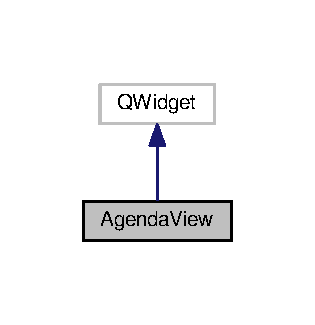
\includegraphics[width=151pt]{class_agenda_view__inherit__graph}
\end{center}
\end{figure}


Collaboration diagram for Agenda\+View\+:\nopagebreak
\begin{figure}[H]
\begin{center}
\leavevmode
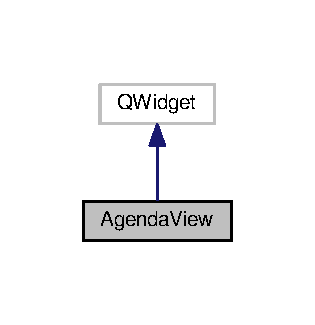
\includegraphics[width=151pt]{class_agenda_view__coll__graph}
\end{center}
\end{figure}
\subsection*{Public Slots}
\begin{DoxyCompactItemize}
\item 
void \hyperlink{class_agenda_view_a4c460ccf9b4764f9422252199b7e8757}{slot\+Events\+Changed} ()
\begin{DoxyCompactList}\small\item\em Appelle l\textquotesingle{}affichage de semaine. \end{DoxyCompactList}\item 
void \hyperlink{class_agenda_view_a28d88cb1a112e93ad768e0846a0a18e6}{slot\+Events\+Changed} (const Q\+Date \&date)
\begin{DoxyCompactList}\small\item\em Appelle l\textquotesingle{}affichage de semaine. \end{DoxyCompactList}\item 
void \hyperlink{class_agenda_view_aff4eae25718bbfa2b1608cffd70341de}{slot\+Exporter} ()
\begin{DoxyCompactList}\small\item\em Appelle l\textquotesingle{}exportation. \end{DoxyCompactList}\end{DoxyCompactItemize}
\subsection*{Public Member Functions}
\begin{DoxyCompactItemize}
\item 
\hyperlink{class_agenda_view_afa7bce9852891d1bad22928c6feb4c5b}{Agenda\+View} (Q\+Widget $\ast$parent=0)
\item 
\hyperlink{class_agenda_view_ad7315a868714d98705c59efa5aa27bde}{$\sim$\+Agenda\+View} ()
\end{DoxyCompactItemize}


\subsection{Detailed Description}
Classe d\textquotesingle{}U\+I gérant le contenu de l\textquotesingle{}onglet Agenda. 

Contient la barre de titre avec le choix de semaine et l\textquotesingle{}exportation ainsi que l\textquotesingle{}ensemble de layouts des jours de la semaine. 

\subsection{Constructor \& Destructor Documentation}
\hypertarget{class_agenda_view_afa7bce9852891d1bad22928c6feb4c5b}{}\index{Agenda\+View@{Agenda\+View}!Agenda\+View@{Agenda\+View}}
\index{Agenda\+View@{Agenda\+View}!Agenda\+View@{Agenda\+View}}
\subsubsection[{Agenda\+View}]{\setlength{\rightskip}{0pt plus 5cm}Agenda\+View\+::\+Agenda\+View (
\begin{DoxyParamCaption}
\item[{Q\+Widget $\ast$}]{parent = {\ttfamily 0}}
\end{DoxyParamCaption}
)\hspace{0.3cm}{\ttfamily [explicit]}}\label{class_agenda_view_afa7bce9852891d1bad22928c6feb4c5b}
\hypertarget{class_agenda_view_ad7315a868714d98705c59efa5aa27bde}{}\index{Agenda\+View@{Agenda\+View}!````~Agenda\+View@{$\sim$\+Agenda\+View}}
\index{````~Agenda\+View@{$\sim$\+Agenda\+View}!Agenda\+View@{Agenda\+View}}
\subsubsection[{$\sim$\+Agenda\+View}]{\setlength{\rightskip}{0pt plus 5cm}Agenda\+View\+::$\sim$\+Agenda\+View (
\begin{DoxyParamCaption}
{}
\end{DoxyParamCaption}
)}\label{class_agenda_view_ad7315a868714d98705c59efa5aa27bde}


\subsection{Member Function Documentation}
\hypertarget{class_agenda_view_a4c460ccf9b4764f9422252199b7e8757}{}\index{Agenda\+View@{Agenda\+View}!slot\+Events\+Changed@{slot\+Events\+Changed}}
\index{slot\+Events\+Changed@{slot\+Events\+Changed}!Agenda\+View@{Agenda\+View}}
\subsubsection[{slot\+Events\+Changed}]{\setlength{\rightskip}{0pt plus 5cm}void Agenda\+View\+::slot\+Events\+Changed (
\begin{DoxyParamCaption}
{}
\end{DoxyParamCaption}
)\hspace{0.3cm}{\ttfamily [slot]}}\label{class_agenda_view_a4c460ccf9b4764f9422252199b7e8757}


Appelle l\textquotesingle{}affichage de semaine. 

\hypertarget{class_agenda_view_a28d88cb1a112e93ad768e0846a0a18e6}{}\index{Agenda\+View@{Agenda\+View}!slot\+Events\+Changed@{slot\+Events\+Changed}}
\index{slot\+Events\+Changed@{slot\+Events\+Changed}!Agenda\+View@{Agenda\+View}}
\subsubsection[{slot\+Events\+Changed}]{\setlength{\rightskip}{0pt plus 5cm}void Agenda\+View\+::slot\+Events\+Changed (
\begin{DoxyParamCaption}
\item[{const Q\+Date \&}]{date}
\end{DoxyParamCaption}
)\hspace{0.3cm}{\ttfamily [slot]}}\label{class_agenda_view_a28d88cb1a112e93ad768e0846a0a18e6}


Appelle l\textquotesingle{}affichage de semaine. 

\hypertarget{class_agenda_view_aff4eae25718bbfa2b1608cffd70341de}{}\index{Agenda\+View@{Agenda\+View}!slot\+Exporter@{slot\+Exporter}}
\index{slot\+Exporter@{slot\+Exporter}!Agenda\+View@{Agenda\+View}}
\subsubsection[{slot\+Exporter}]{\setlength{\rightskip}{0pt plus 5cm}void Agenda\+View\+::slot\+Exporter (
\begin{DoxyParamCaption}
{}
\end{DoxyParamCaption}
)\hspace{0.3cm}{\ttfamily [slot]}}\label{class_agenda_view_aff4eae25718bbfa2b1608cffd70341de}


Appelle l\textquotesingle{}exportation. 



The documentation for this class was generated from the following files\+:\begin{DoxyCompactItemize}
\item 
L\+O21app/\hyperlink{agendaview_8h}{agendaview.\+h}\item 
L\+O21app/\hyperlink{agendaview_8cpp}{agendaview.\+cpp}\end{DoxyCompactItemize}

\hypertarget{class_calendar_exception}{}\section{Calendar\+Exception Class Reference}
\label{class_calendar_exception}\index{Calendar\+Exception@{Calendar\+Exception}}


Classe d\textquotesingle{}affichage des erreurs.  




{\ttfamily \#include $<$Calendar.\+h$>$}

\subsection*{Public Member Functions}
\begin{DoxyCompactItemize}
\item 
\hypertarget{class_calendar_exception_af4a976332f7659bdd866926f0145a780}{}{\bfseries Calendar\+Exception} (const string \&message)\label{class_calendar_exception_af4a976332f7659bdd866926f0145a780}

\item 
\hypertarget{class_calendar_exception_a381389e24c3efae51565bc4e7865a7d6}{}string {\bfseries get\+Info} () const \label{class_calendar_exception_a381389e24c3efae51565bc4e7865a7d6}

\end{DoxyCompactItemize}


\subsection{Detailed Description}
Classe d\textquotesingle{}affichage des erreurs. 

The documentation for this class was generated from the following file\+:\begin{DoxyCompactItemize}
\item 
L\+O21app/Calendar.\+h\end{DoxyCompactItemize}

\hypertarget{class_composite_1_1_compo_iterator}{}\section{Composite\+:\+:Compo\+Iterator Class Reference}
\label{class_composite_1_1_compo_iterator}\index{Composite\+::\+Compo\+Iterator@{Composite\+::\+Compo\+Iterator}}


{\ttfamily \#include $<$Calendar.\+h$>$}

\subsection*{Public Member Functions}
\begin{DoxyCompactItemize}
\item 
\hyperlink{class_tache}{Tache} \& \hyperlink{class_composite_1_1_compo_iterator_a7aaef00a1f93480d0a7b4536de684e1f}{current} () const 
\item 
bool \hyperlink{class_composite_1_1_compo_iterator_ad6d9bf86b4a38f7a0bbb09dbf8586882}{is\+Done} () const 
\item 
void \hyperlink{class_composite_1_1_compo_iterator_aafb960ce0debec3d8dc6288a67e03439}{next} ()
\item 
void \hyperlink{class_composite_1_1_compo_iterator_a4338d376134b3250cd3892042b70b0f1}{first} ()
\end{DoxyCompactItemize}
\subsection*{Friends}
\begin{DoxyCompactItemize}
\item 
class \hyperlink{class_composite_1_1_compo_iterator_ace19a20e83d0e04d1929284108a7582d}{Composite}
\end{DoxyCompactItemize}


\subsection{Member Function Documentation}
\hypertarget{class_composite_1_1_compo_iterator_a7aaef00a1f93480d0a7b4536de684e1f}{}\index{Composite\+::\+Compo\+Iterator@{Composite\+::\+Compo\+Iterator}!current@{current}}
\index{current@{current}!Composite\+::\+Compo\+Iterator@{Composite\+::\+Compo\+Iterator}}
\subsubsection[{current}]{\setlength{\rightskip}{0pt plus 5cm}{\bf Tache}\& Composite\+::\+Compo\+Iterator\+::current (
\begin{DoxyParamCaption}
{}
\end{DoxyParamCaption}
) const\hspace{0.3cm}{\ttfamily [inline]}}\label{class_composite_1_1_compo_iterator_a7aaef00a1f93480d0a7b4536de684e1f}
\hypertarget{class_composite_1_1_compo_iterator_a4338d376134b3250cd3892042b70b0f1}{}\index{Composite\+::\+Compo\+Iterator@{Composite\+::\+Compo\+Iterator}!first@{first}}
\index{first@{first}!Composite\+::\+Compo\+Iterator@{Composite\+::\+Compo\+Iterator}}
\subsubsection[{first}]{\setlength{\rightskip}{0pt plus 5cm}void Composite\+::\+Compo\+Iterator\+::first (
\begin{DoxyParamCaption}
{}
\end{DoxyParamCaption}
)\hspace{0.3cm}{\ttfamily [inline]}}\label{class_composite_1_1_compo_iterator_a4338d376134b3250cd3892042b70b0f1}
\hypertarget{class_composite_1_1_compo_iterator_ad6d9bf86b4a38f7a0bbb09dbf8586882}{}\index{Composite\+::\+Compo\+Iterator@{Composite\+::\+Compo\+Iterator}!is\+Done@{is\+Done}}
\index{is\+Done@{is\+Done}!Composite\+::\+Compo\+Iterator@{Composite\+::\+Compo\+Iterator}}
\subsubsection[{is\+Done}]{\setlength{\rightskip}{0pt plus 5cm}bool Composite\+::\+Compo\+Iterator\+::is\+Done (
\begin{DoxyParamCaption}
{}
\end{DoxyParamCaption}
) const\hspace{0.3cm}{\ttfamily [inline]}}\label{class_composite_1_1_compo_iterator_ad6d9bf86b4a38f7a0bbb09dbf8586882}
\hypertarget{class_composite_1_1_compo_iterator_aafb960ce0debec3d8dc6288a67e03439}{}\index{Composite\+::\+Compo\+Iterator@{Composite\+::\+Compo\+Iterator}!next@{next}}
\index{next@{next}!Composite\+::\+Compo\+Iterator@{Composite\+::\+Compo\+Iterator}}
\subsubsection[{next}]{\setlength{\rightskip}{0pt plus 5cm}void Composite\+::\+Compo\+Iterator\+::next (
\begin{DoxyParamCaption}
{}
\end{DoxyParamCaption}
)\hspace{0.3cm}{\ttfamily [inline]}}\label{class_composite_1_1_compo_iterator_aafb960ce0debec3d8dc6288a67e03439}


\subsection{Friends And Related Function Documentation}
\hypertarget{class_composite_1_1_compo_iterator_ace19a20e83d0e04d1929284108a7582d}{}\index{Composite\+::\+Compo\+Iterator@{Composite\+::\+Compo\+Iterator}!Composite@{Composite}}
\index{Composite@{Composite}!Composite\+::\+Compo\+Iterator@{Composite\+::\+Compo\+Iterator}}
\subsubsection[{Composite}]{\setlength{\rightskip}{0pt plus 5cm}friend class {\bf Composite}\hspace{0.3cm}{\ttfamily [friend]}}\label{class_composite_1_1_compo_iterator_ace19a20e83d0e04d1929284108a7582d}


The documentation for this class was generated from the following file\+:\begin{DoxyCompactItemize}
\item 
L\+O21app/\hyperlink{_calendar_8h}{Calendar.\+h}\end{DoxyCompactItemize}

\hypertarget{class_composite}{}\section{Composite Class Reference}
\label{class_composite}\index{Composite@{Composite}}


\hyperlink{class_tache}{Tache} qui peut contenir des tâches mais ne peut pas être programmée.  




{\ttfamily \#include $<$Calendar.\+h$>$}



Inheritance diagram for Composite\+:\nopagebreak
\begin{figure}[H]
\begin{center}
\leavevmode
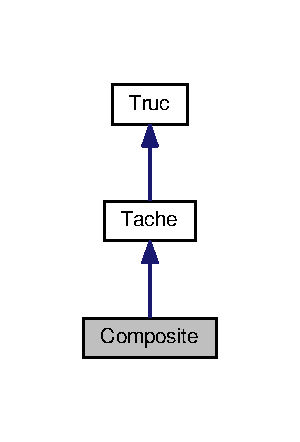
\includegraphics[width=144pt]{class_composite__inherit__graph}
\end{center}
\end{figure}


Collaboration diagram for Composite\+:\nopagebreak
\begin{figure}[H]
\begin{center}
\leavevmode
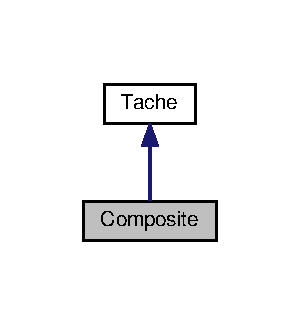
\includegraphics[width=186pt]{class_composite__coll__graph}
\end{center}
\end{figure}
\subsection*{Classes}
\begin{DoxyCompactItemize}
\item 
class \hyperlink{class_composite_1_1iterator}{iterator}
\end{DoxyCompactItemize}
\subsection*{Public Member Functions}
\begin{DoxyCompactItemize}
\item 
\hypertarget{class_composite_a63c52493ad8add53951157a418fa0971}{}\hyperlink{class_composite_1_1iterator}{iterator} {\bfseries getiterator} ()\label{class_composite_a63c52493ad8add53951157a418fa0971}

\end{DoxyCompactItemize}
\subsection*{Friends}
\begin{DoxyCompactItemize}
\item 
\hypertarget{class_composite_a67171474c4da6cc8efe0c7fafefd2b2d}{}class {\bfseries iterator}\label{class_composite_a67171474c4da6cc8efe0c7fafefd2b2d}

\end{DoxyCompactItemize}
\subsection*{Additional Inherited Members}


\subsection{Detailed Description}
\hyperlink{class_tache}{Tache} qui peut contenir des tâches mais ne peut pas être programmée. 

The documentation for this class was generated from the following file\+:\begin{DoxyCompactItemize}
\item 
L\+O21app/Calendar.\+h\end{DoxyCompactItemize}

\hypertarget{class_t_i_m_e_1_1_date}{}\section{T\+I\+M\+E\+:\+:Date Class Reference}
\label{class_t_i_m_e_1_1_date}\index{T\+I\+M\+E\+::\+Date@{T\+I\+M\+E\+::\+Date}}


Classe permettant de manipuler des dates standards L\textquotesingle{}utilisation de cette classe n�cessite des dates valides au sens commun du terme. D�clenchement d\textquotesingle{}exception dans le cas contraire.  




{\ttfamily \#include $<$timing.\+h$>$}

\subsection*{Public Member Functions}
\begin{DoxyCompactItemize}
\item 
\hyperlink{class_t_i_m_e_1_1_date_ab0d72ce6e986c0c0a5f2902e586cf81a}{Date} (unsigned int short j=1, unsigned int short m=1, unsigned int a=0)
\begin{DoxyCompactList}\small\item\em Constructeur � partir d\textquotesingle{}un jour, mois, ann�e. \end{DoxyCompactList}\item 
unsigned short int \hyperlink{class_t_i_m_e_1_1_date_a4af978b7df2b738f62449b0a7e53c21d}{get\+Jour} () const 
\begin{DoxyCompactList}\small\item\em Retourne le jour de la date. \end{DoxyCompactList}\item 
unsigned short int \hyperlink{class_t_i_m_e_1_1_date_a6cb9d945143df216115419c4cb8b14ce}{get\+Mois} () const 
\begin{DoxyCompactList}\small\item\em Retourne le mois de la date. \end{DoxyCompactList}\item 
unsigned int \hyperlink{class_t_i_m_e_1_1_date_a07b41b2e9e85ef78bf13689e772bef7d}{get\+Annee} () const 
\begin{DoxyCompactList}\small\item\em Retourne l\textquotesingle{}ann�e de la date. \end{DoxyCompactList}\item 
Q\+Date \hyperlink{class_t_i_m_e_1_1_date_a30428bf3b5e4daa144642dfa510edb14}{get\+Q\+Date} () const 
\begin{DoxyCompactList}\small\item\em Retourne l\textquotesingle{}ann�e de la date. \end{DoxyCompactList}\item 
std\+::string \hyperlink{class_t_i_m_e_1_1_date_a09b00b96742bfceaa598060b486e604c}{get\+Jour\+Mois\+String} () const 
\begin{DoxyCompactList}\small\item\em initialisation de la date \end{DoxyCompactList}\item 
void \hyperlink{class_t_i_m_e_1_1_date_a7419902750e61b9473ab05ccd5ced33d}{set\+Date} (unsigned short int j, unsigned short int m, unsigned int a)
\begin{DoxyCompactList}\small\item\em initialisation de la date avec la date d\textquotesingle{}aujourd\textquotesingle{}hui \end{DoxyCompactList}\item 
void \hyperlink{class_t_i_m_e_1_1_date_ace4be52a503c45de93b8db92dc592d93}{set\+Date\+Aujourdhui} ()
\begin{DoxyCompactList}\small\item\em affiche le date sous le format J\+J/\+M\+M/\+A\+A\+A\+A \end{DoxyCompactList}\item 
void \hyperlink{class_t_i_m_e_1_1_date_aa45188755f5d9d17cbebf0e55d3c571b}{afficher} (std\+::ostream \&f=std\+::cout) const 
\item 
bool \hyperlink{class_t_i_m_e_1_1_date_aa8208298c0efe5dbf661c66a284fd163}{operator==} (const \hyperlink{class_t_i_m_e_1_1_date}{Date} \&d) const 
\begin{DoxyCompactList}\small\item\em d1==d2 retourne vrai si les deux dates sont �gales \end{DoxyCompactList}\item 
bool \hyperlink{class_t_i_m_e_1_1_date_a8a3bccb05f00086e64c5b5518a37949f}{operator$<$} (const \hyperlink{class_t_i_m_e_1_1_date}{Date} \&d) const 
\begin{DoxyCompactList}\small\item\em Compare deux dates dans le temps \+: d1$<$d2 retourne true si d1 est avant d2. \end{DoxyCompactList}\item 
bool \hyperlink{class_t_i_m_e_1_1_date_a4e6d6c380ef57bd34506ba8f017fec67}{operator$<$=} (const \hyperlink{class_t_i_m_e_1_1_date}{Date} \&d) const 
\begin{DoxyCompactList}\small\item\em Compare deux dates dans le temps \+: d1$<$=d2 retourne true si d1 est avant ou bien �gale � d2. \end{DoxyCompactList}\item 
int \hyperlink{class_t_i_m_e_1_1_date_a61f93f8612a998bc440070f9b8a2660a}{operator-\/} (const \hyperlink{class_t_i_m_e_1_1_date}{Date} \&d) const 
\begin{DoxyCompactList}\small\item\em Retourne le nombre de jours s�parant les deux dates. \end{DoxyCompactList}\item 
\hyperlink{class_t_i_m_e_1_1_date}{Date} \hyperlink{class_t_i_m_e_1_1_date_a85907da4cadaff930c748328fda4d527}{demain} () const 
\begin{DoxyCompactList}\small\item\em Retourne la date du lendemain. \end{DoxyCompactList}\item 
\hyperlink{class_t_i_m_e_1_1_date}{Date} \hyperlink{class_t_i_m_e_1_1_date_a3c1f346c2ad9287155a71dc5d09e7fd8}{operator+} (unsigned int nb) const 
\begin{DoxyCompactList}\small\item\em Retourne la date de dans nb jours. \end{DoxyCompactList}\end{DoxyCompactItemize}
\subsection*{Static Public Member Functions}
\begin{DoxyCompactItemize}
\item 
static \hyperlink{class_t_i_m_e_1_1_date}{Date} \hyperlink{class_t_i_m_e_1_1_date_a17bb8fb342545a476f35fe745613f7a9}{to\+Timing\+Date} (Q\+Date d)
\end{DoxyCompactItemize}


\subsection{Detailed Description}
Classe permettant de manipuler des dates standards L\textquotesingle{}utilisation de cette classe n�cessite des dates valides au sens commun du terme. D�clenchement d\textquotesingle{}exception dans le cas contraire. 

\subsection{Constructor \& Destructor Documentation}
\hypertarget{class_t_i_m_e_1_1_date_ab0d72ce6e986c0c0a5f2902e586cf81a}{}\index{T\+I\+M\+E\+::\+Date@{T\+I\+M\+E\+::\+Date}!Date@{Date}}
\index{Date@{Date}!T\+I\+M\+E\+::\+Date@{T\+I\+M\+E\+::\+Date}}
\subsubsection[{Date}]{\setlength{\rightskip}{0pt plus 5cm}T\+I\+M\+E\+::\+Date\+::\+Date (
\begin{DoxyParamCaption}
\item[{unsigned int short}]{j = {\ttfamily 1}, }
\item[{unsigned int short}]{m = {\ttfamily 1}, }
\item[{unsigned int}]{a = {\ttfamily 0}}
\end{DoxyParamCaption}
)\hspace{0.3cm}{\ttfamily [inline]}}\label{class_t_i_m_e_1_1_date_ab0d72ce6e986c0c0a5f2902e586cf81a}


Constructeur � partir d\textquotesingle{}un jour, mois, ann�e. 


\begin{DoxyParams}{Parameters}
{\em j} & jour avec 1$<$=j$<$=31 \\
\hline
{\em m} & mois avec 1$<$=m$<$=12 \\
\hline
{\em a} & ann�e avec a$>$=0 \\
\hline
\end{DoxyParams}


\subsection{Member Function Documentation}
\hypertarget{class_t_i_m_e_1_1_date_aa45188755f5d9d17cbebf0e55d3c571b}{}\index{T\+I\+M\+E\+::\+Date@{T\+I\+M\+E\+::\+Date}!afficher@{afficher}}
\index{afficher@{afficher}!T\+I\+M\+E\+::\+Date@{T\+I\+M\+E\+::\+Date}}
\subsubsection[{afficher}]{\setlength{\rightskip}{0pt plus 5cm}void Date\+::afficher (
\begin{DoxyParamCaption}
\item[{std\+::ostream \&}]{f = {\ttfamily std\+:\+:cout}}
\end{DoxyParamCaption}
) const}\label{class_t_i_m_e_1_1_date_aa45188755f5d9d17cbebf0e55d3c571b}
\hypertarget{class_t_i_m_e_1_1_date_a85907da4cadaff930c748328fda4d527}{}\index{T\+I\+M\+E\+::\+Date@{T\+I\+M\+E\+::\+Date}!demain@{demain}}
\index{demain@{demain}!T\+I\+M\+E\+::\+Date@{T\+I\+M\+E\+::\+Date}}
\subsubsection[{demain}]{\setlength{\rightskip}{0pt plus 5cm}{\bf Date} Date\+::demain (
\begin{DoxyParamCaption}
{}
\end{DoxyParamCaption}
) const}\label{class_t_i_m_e_1_1_date_a85907da4cadaff930c748328fda4d527}


Retourne la date du lendemain. 

\hypertarget{class_t_i_m_e_1_1_date_a07b41b2e9e85ef78bf13689e772bef7d}{}\index{T\+I\+M\+E\+::\+Date@{T\+I\+M\+E\+::\+Date}!get\+Annee@{get\+Annee}}
\index{get\+Annee@{get\+Annee}!T\+I\+M\+E\+::\+Date@{T\+I\+M\+E\+::\+Date}}
\subsubsection[{get\+Annee}]{\setlength{\rightskip}{0pt plus 5cm}unsigned int T\+I\+M\+E\+::\+Date\+::get\+Annee (
\begin{DoxyParamCaption}
{}
\end{DoxyParamCaption}
) const\hspace{0.3cm}{\ttfamily [inline]}}\label{class_t_i_m_e_1_1_date_a07b41b2e9e85ef78bf13689e772bef7d}


Retourne l\textquotesingle{}ann�e de la date. 

\hypertarget{class_t_i_m_e_1_1_date_a4af978b7df2b738f62449b0a7e53c21d}{}\index{T\+I\+M\+E\+::\+Date@{T\+I\+M\+E\+::\+Date}!get\+Jour@{get\+Jour}}
\index{get\+Jour@{get\+Jour}!T\+I\+M\+E\+::\+Date@{T\+I\+M\+E\+::\+Date}}
\subsubsection[{get\+Jour}]{\setlength{\rightskip}{0pt plus 5cm}unsigned short int T\+I\+M\+E\+::\+Date\+::get\+Jour (
\begin{DoxyParamCaption}
{}
\end{DoxyParamCaption}
) const\hspace{0.3cm}{\ttfamily [inline]}}\label{class_t_i_m_e_1_1_date_a4af978b7df2b738f62449b0a7e53c21d}


Retourne le jour de la date. 

\hypertarget{class_t_i_m_e_1_1_date_a09b00b96742bfceaa598060b486e604c}{}\index{T\+I\+M\+E\+::\+Date@{T\+I\+M\+E\+::\+Date}!get\+Jour\+Mois\+String@{get\+Jour\+Mois\+String}}
\index{get\+Jour\+Mois\+String@{get\+Jour\+Mois\+String}!T\+I\+M\+E\+::\+Date@{T\+I\+M\+E\+::\+Date}}
\subsubsection[{get\+Jour\+Mois\+String}]{\setlength{\rightskip}{0pt plus 5cm}std\+::string T\+I\+M\+E\+::\+Date\+::get\+Jour\+Mois\+String (
\begin{DoxyParamCaption}
{}
\end{DoxyParamCaption}
) const\hspace{0.3cm}{\ttfamily [inline]}}\label{class_t_i_m_e_1_1_date_a09b00b96742bfceaa598060b486e604c}


initialisation de la date 

Retourne l\textquotesingle{}heure sous forme de chaine \hypertarget{class_t_i_m_e_1_1_date_a6cb9d945143df216115419c4cb8b14ce}{}\index{T\+I\+M\+E\+::\+Date@{T\+I\+M\+E\+::\+Date}!get\+Mois@{get\+Mois}}
\index{get\+Mois@{get\+Mois}!T\+I\+M\+E\+::\+Date@{T\+I\+M\+E\+::\+Date}}
\subsubsection[{get\+Mois}]{\setlength{\rightskip}{0pt plus 5cm}unsigned short int T\+I\+M\+E\+::\+Date\+::get\+Mois (
\begin{DoxyParamCaption}
{}
\end{DoxyParamCaption}
) const\hspace{0.3cm}{\ttfamily [inline]}}\label{class_t_i_m_e_1_1_date_a6cb9d945143df216115419c4cb8b14ce}


Retourne le mois de la date. 

\hypertarget{class_t_i_m_e_1_1_date_a30428bf3b5e4daa144642dfa510edb14}{}\index{T\+I\+M\+E\+::\+Date@{T\+I\+M\+E\+::\+Date}!get\+Q\+Date@{get\+Q\+Date}}
\index{get\+Q\+Date@{get\+Q\+Date}!T\+I\+M\+E\+::\+Date@{T\+I\+M\+E\+::\+Date}}
\subsubsection[{get\+Q\+Date}]{\setlength{\rightskip}{0pt plus 5cm}Q\+Date T\+I\+M\+E\+::\+Date\+::get\+Q\+Date (
\begin{DoxyParamCaption}
{}
\end{DoxyParamCaption}
) const\hspace{0.3cm}{\ttfamily [inline]}}\label{class_t_i_m_e_1_1_date_a30428bf3b5e4daa144642dfa510edb14}


Retourne l\textquotesingle{}ann�e de la date. 

\hypertarget{class_t_i_m_e_1_1_date_a3c1f346c2ad9287155a71dc5d09e7fd8}{}\index{T\+I\+M\+E\+::\+Date@{T\+I\+M\+E\+::\+Date}!operator+@{operator+}}
\index{operator+@{operator+}!T\+I\+M\+E\+::\+Date@{T\+I\+M\+E\+::\+Date}}
\subsubsection[{operator+}]{\setlength{\rightskip}{0pt plus 5cm}{\bf Date} Date\+::operator+ (
\begin{DoxyParamCaption}
\item[{unsigned int}]{nb}
\end{DoxyParamCaption}
) const}\label{class_t_i_m_e_1_1_date_a3c1f346c2ad9287155a71dc5d09e7fd8}


Retourne la date de dans nb jours. 

\hypertarget{class_t_i_m_e_1_1_date_a61f93f8612a998bc440070f9b8a2660a}{}\index{T\+I\+M\+E\+::\+Date@{T\+I\+M\+E\+::\+Date}!operator-\/@{operator-\/}}
\index{operator-\/@{operator-\/}!T\+I\+M\+E\+::\+Date@{T\+I\+M\+E\+::\+Date}}
\subsubsection[{operator-\/}]{\setlength{\rightskip}{0pt plus 5cm}int Date\+::operator-\/ (
\begin{DoxyParamCaption}
\item[{const {\bf Date} \&}]{d}
\end{DoxyParamCaption}
) const}\label{class_t_i_m_e_1_1_date_a61f93f8612a998bc440070f9b8a2660a}


Retourne le nombre de jours s�parant les deux dates. 

\hypertarget{class_t_i_m_e_1_1_date_a8a3bccb05f00086e64c5b5518a37949f}{}\index{T\+I\+M\+E\+::\+Date@{T\+I\+M\+E\+::\+Date}!operator$<$@{operator$<$}}
\index{operator$<$@{operator$<$}!T\+I\+M\+E\+::\+Date@{T\+I\+M\+E\+::\+Date}}
\subsubsection[{operator$<$}]{\setlength{\rightskip}{0pt plus 5cm}bool Date\+::operator$<$ (
\begin{DoxyParamCaption}
\item[{const {\bf Date} \&}]{d}
\end{DoxyParamCaption}
) const}\label{class_t_i_m_e_1_1_date_a8a3bccb05f00086e64c5b5518a37949f}


Compare deux dates dans le temps \+: d1$<$d2 retourne true si d1 est avant d2. 

\hypertarget{class_t_i_m_e_1_1_date_a4e6d6c380ef57bd34506ba8f017fec67}{}\index{T\+I\+M\+E\+::\+Date@{T\+I\+M\+E\+::\+Date}!operator$<$=@{operator$<$=}}
\index{operator$<$=@{operator$<$=}!T\+I\+M\+E\+::\+Date@{T\+I\+M\+E\+::\+Date}}
\subsubsection[{operator$<$=}]{\setlength{\rightskip}{0pt plus 5cm}bool Date\+::operator$<$= (
\begin{DoxyParamCaption}
\item[{const {\bf Date} \&}]{d}
\end{DoxyParamCaption}
) const}\label{class_t_i_m_e_1_1_date_a4e6d6c380ef57bd34506ba8f017fec67}


Compare deux dates dans le temps \+: d1$<$=d2 retourne true si d1 est avant ou bien �gale � d2. 

\hypertarget{class_t_i_m_e_1_1_date_aa8208298c0efe5dbf661c66a284fd163}{}\index{T\+I\+M\+E\+::\+Date@{T\+I\+M\+E\+::\+Date}!operator==@{operator==}}
\index{operator==@{operator==}!T\+I\+M\+E\+::\+Date@{T\+I\+M\+E\+::\+Date}}
\subsubsection[{operator==}]{\setlength{\rightskip}{0pt plus 5cm}bool Date\+::operator== (
\begin{DoxyParamCaption}
\item[{const {\bf Date} \&}]{d}
\end{DoxyParamCaption}
) const}\label{class_t_i_m_e_1_1_date_aa8208298c0efe5dbf661c66a284fd163}


d1==d2 retourne vrai si les deux dates sont �gales 

\hypertarget{class_t_i_m_e_1_1_date_a7419902750e61b9473ab05ccd5ced33d}{}\index{T\+I\+M\+E\+::\+Date@{T\+I\+M\+E\+::\+Date}!set\+Date@{set\+Date}}
\index{set\+Date@{set\+Date}!T\+I\+M\+E\+::\+Date@{T\+I\+M\+E\+::\+Date}}
\subsubsection[{set\+Date}]{\setlength{\rightskip}{0pt plus 5cm}void Date\+::set\+Date (
\begin{DoxyParamCaption}
\item[{unsigned short int}]{j, }
\item[{unsigned short int}]{m, }
\item[{unsigned int}]{a}
\end{DoxyParamCaption}
)}\label{class_t_i_m_e_1_1_date_a7419902750e61b9473ab05ccd5ced33d}


initialisation de la date avec la date d\textquotesingle{}aujourd\textquotesingle{}hui 

\hypertarget{class_t_i_m_e_1_1_date_ace4be52a503c45de93b8db92dc592d93}{}\index{T\+I\+M\+E\+::\+Date@{T\+I\+M\+E\+::\+Date}!set\+Date\+Aujourdhui@{set\+Date\+Aujourdhui}}
\index{set\+Date\+Aujourdhui@{set\+Date\+Aujourdhui}!T\+I\+M\+E\+::\+Date@{T\+I\+M\+E\+::\+Date}}
\subsubsection[{set\+Date\+Aujourdhui}]{\setlength{\rightskip}{0pt plus 5cm}void Date\+::set\+Date\+Aujourdhui (
\begin{DoxyParamCaption}
{}
\end{DoxyParamCaption}
)}\label{class_t_i_m_e_1_1_date_ace4be52a503c45de93b8db92dc592d93}


affiche le date sous le format J\+J/\+M\+M/\+A\+A\+A\+A 

\hypertarget{class_t_i_m_e_1_1_date_a17bb8fb342545a476f35fe745613f7a9}{}\index{T\+I\+M\+E\+::\+Date@{T\+I\+M\+E\+::\+Date}!to\+Timing\+Date@{to\+Timing\+Date}}
\index{to\+Timing\+Date@{to\+Timing\+Date}!T\+I\+M\+E\+::\+Date@{T\+I\+M\+E\+::\+Date}}
\subsubsection[{to\+Timing\+Date}]{\setlength{\rightskip}{0pt plus 5cm}{\bf Date} Date\+::to\+Timing\+Date (
\begin{DoxyParamCaption}
\item[{Q\+Date}]{d}
\end{DoxyParamCaption}
)\hspace{0.3cm}{\ttfamily [static]}}\label{class_t_i_m_e_1_1_date_a17bb8fb342545a476f35fe745613f7a9}


The documentation for this class was generated from the following files\+:\begin{DoxyCompactItemize}
\item 
L\+O21app/\hyperlink{timing_8h}{timing.\+h}\item 
L\+O21app/\hyperlink{timing_8cpp}{timing.\+cpp}\end{DoxyCompactItemize}

\hypertarget{class_t_i_m_e_1_1_duree}{}\section{T\+I\+M\+E\+:\+:Duree Class Reference}
\label{class_t_i_m_e_1_1_duree}\index{T\+I\+M\+E\+::\+Duree@{T\+I\+M\+E\+::\+Duree}}


Classe permettant de manipuler des durees L\textquotesingle{}utilisation de cette classe n�cessite des dates valides au sens commun du terme. D�clenchement d\textquotesingle{}exception dans le cas contraire.  




{\ttfamily \#include $<$timing.\+h$>$}

\subsection*{Public Member Functions}
\begin{DoxyCompactItemize}
\item 
\hyperlink{class_t_i_m_e_1_1_duree_ae0532a0d60dbc31773f038967dfe220e}{Duree} (unsigned int h, unsigned int m)
\begin{DoxyCompactList}\small\item\em Constructeur � partir de heure et minute. \end{DoxyCompactList}\item 
\hyperlink{class_t_i_m_e_1_1_duree_a0f99878e52fad2f9e0643301c70d9ef7}{Duree} (unsigned int m=0)
\begin{DoxyCompactList}\small\item\em Constructeur � partir de minute. \end{DoxyCompactList}\item 
void \hyperlink{class_t_i_m_e_1_1_duree_aabba3e357861f21faa8419339f7b7176}{set\+Duree} (unsigned int heures, unsigned int minutes)
\item 
unsigned int \hyperlink{class_t_i_m_e_1_1_duree_a1e47fb5f0734ec562e2f9dba32db45f4}{get\+Duree\+En\+Minutes} () const 
\begin{DoxyCompactList}\small\item\em Retourne la duree en minutes. \end{DoxyCompactList}\item 
double \hyperlink{class_t_i_m_e_1_1_duree_afb11d106fc1f6761a68f486dc7a17564}{get\+Duree\+En\+Heures} () const 
\begin{DoxyCompactList}\small\item\em Retourne la duree en heures. \end{DoxyCompactList}\item 
unsigned int \hyperlink{class_t_i_m_e_1_1_duree_aeb43e9bde7803d89edbabf040c962f9b}{get\+Duree\+En\+Heures\+Int} () const 
\begin{DoxyCompactList}\small\item\em Retourne la duree en heures tronqu�e � l\textquotesingle{}heure pr�s. \end{DoxyCompactList}\item 
void \hyperlink{class_t_i_m_e_1_1_duree_ad957a58f8bc103857f3e494bab5f60e1}{afficher} (std\+::ostream \&f=std\+::cout) const 
\begin{DoxyCompactList}\small\item\em Affiche la duree sous le format hh\+Hmm. \end{DoxyCompactList}\item 
bool \hyperlink{class_t_i_m_e_1_1_duree_a96ac8dafc768f4c52d6811a5a89cafbc}{is\+Null} ()
\end{DoxyCompactItemize}


\subsection{Detailed Description}
Classe permettant de manipuler des durees L\textquotesingle{}utilisation de cette classe n�cessite des dates valides au sens commun du terme. D�clenchement d\textquotesingle{}exception dans le cas contraire. 

\subsection{Constructor \& Destructor Documentation}
\hypertarget{class_t_i_m_e_1_1_duree_ae0532a0d60dbc31773f038967dfe220e}{}\index{T\+I\+M\+E\+::\+Duree@{T\+I\+M\+E\+::\+Duree}!Duree@{Duree}}
\index{Duree@{Duree}!T\+I\+M\+E\+::\+Duree@{T\+I\+M\+E\+::\+Duree}}
\subsubsection[{Duree}]{\setlength{\rightskip}{0pt plus 5cm}T\+I\+M\+E\+::\+Duree\+::\+Duree (
\begin{DoxyParamCaption}
\item[{unsigned int}]{h, }
\item[{unsigned int}]{m}
\end{DoxyParamCaption}
)\hspace{0.3cm}{\ttfamily [inline]}}\label{class_t_i_m_e_1_1_duree_ae0532a0d60dbc31773f038967dfe220e}


Constructeur � partir de heure et minute. 


\begin{DoxyParams}{Parameters}
{\em h} & heure avec h$>$=0 \\
\hline
{\em m} & minute avec 0$<$=m$<$=59 \\
\hline
\end{DoxyParams}
\hypertarget{class_t_i_m_e_1_1_duree_a0f99878e52fad2f9e0643301c70d9ef7}{}\index{T\+I\+M\+E\+::\+Duree@{T\+I\+M\+E\+::\+Duree}!Duree@{Duree}}
\index{Duree@{Duree}!T\+I\+M\+E\+::\+Duree@{T\+I\+M\+E\+::\+Duree}}
\subsubsection[{Duree}]{\setlength{\rightskip}{0pt plus 5cm}T\+I\+M\+E\+::\+Duree\+::\+Duree (
\begin{DoxyParamCaption}
\item[{unsigned int}]{m = {\ttfamily 0}}
\end{DoxyParamCaption}
)\hspace{0.3cm}{\ttfamily [inline]}}\label{class_t_i_m_e_1_1_duree_a0f99878e52fad2f9e0643301c70d9ef7}


Constructeur � partir de minute. 


\begin{DoxyParams}{Parameters}
{\em m} & minute avec m$>$=0 \\
\hline
\end{DoxyParams}


\subsection{Member Function Documentation}
\hypertarget{class_t_i_m_e_1_1_duree_ad957a58f8bc103857f3e494bab5f60e1}{}\index{T\+I\+M\+E\+::\+Duree@{T\+I\+M\+E\+::\+Duree}!afficher@{afficher}}
\index{afficher@{afficher}!T\+I\+M\+E\+::\+Duree@{T\+I\+M\+E\+::\+Duree}}
\subsubsection[{afficher}]{\setlength{\rightskip}{0pt plus 5cm}void T\+I\+M\+E\+::\+Duree\+::afficher (
\begin{DoxyParamCaption}
\item[{std\+::ostream \&}]{f = {\ttfamily std\+:\+:cout}}
\end{DoxyParamCaption}
) const\hspace{0.3cm}{\ttfamily [inline]}}\label{class_t_i_m_e_1_1_duree_ad957a58f8bc103857f3e494bab5f60e1}


Affiche la duree sous le format hh\+Hmm. 

\hypertarget{class_t_i_m_e_1_1_duree_afb11d106fc1f6761a68f486dc7a17564}{}\index{T\+I\+M\+E\+::\+Duree@{T\+I\+M\+E\+::\+Duree}!get\+Duree\+En\+Heures@{get\+Duree\+En\+Heures}}
\index{get\+Duree\+En\+Heures@{get\+Duree\+En\+Heures}!T\+I\+M\+E\+::\+Duree@{T\+I\+M\+E\+::\+Duree}}
\subsubsection[{get\+Duree\+En\+Heures}]{\setlength{\rightskip}{0pt plus 5cm}double T\+I\+M\+E\+::\+Duree\+::get\+Duree\+En\+Heures (
\begin{DoxyParamCaption}
{}
\end{DoxyParamCaption}
) const\hspace{0.3cm}{\ttfamily [inline]}}\label{class_t_i_m_e_1_1_duree_afb11d106fc1f6761a68f486dc7a17564}


Retourne la duree en heures. 

\hypertarget{class_t_i_m_e_1_1_duree_aeb43e9bde7803d89edbabf040c962f9b}{}\index{T\+I\+M\+E\+::\+Duree@{T\+I\+M\+E\+::\+Duree}!get\+Duree\+En\+Heures\+Int@{get\+Duree\+En\+Heures\+Int}}
\index{get\+Duree\+En\+Heures\+Int@{get\+Duree\+En\+Heures\+Int}!T\+I\+M\+E\+::\+Duree@{T\+I\+M\+E\+::\+Duree}}
\subsubsection[{get\+Duree\+En\+Heures\+Int}]{\setlength{\rightskip}{0pt plus 5cm}unsigned int T\+I\+M\+E\+::\+Duree\+::get\+Duree\+En\+Heures\+Int (
\begin{DoxyParamCaption}
{}
\end{DoxyParamCaption}
) const\hspace{0.3cm}{\ttfamily [inline]}}\label{class_t_i_m_e_1_1_duree_aeb43e9bde7803d89edbabf040c962f9b}


Retourne la duree en heures tronqu�e � l\textquotesingle{}heure pr�s. 

\hypertarget{class_t_i_m_e_1_1_duree_a1e47fb5f0734ec562e2f9dba32db45f4}{}\index{T\+I\+M\+E\+::\+Duree@{T\+I\+M\+E\+::\+Duree}!get\+Duree\+En\+Minutes@{get\+Duree\+En\+Minutes}}
\index{get\+Duree\+En\+Minutes@{get\+Duree\+En\+Minutes}!T\+I\+M\+E\+::\+Duree@{T\+I\+M\+E\+::\+Duree}}
\subsubsection[{get\+Duree\+En\+Minutes}]{\setlength{\rightskip}{0pt plus 5cm}unsigned int T\+I\+M\+E\+::\+Duree\+::get\+Duree\+En\+Minutes (
\begin{DoxyParamCaption}
{}
\end{DoxyParamCaption}
) const\hspace{0.3cm}{\ttfamily [inline]}}\label{class_t_i_m_e_1_1_duree_a1e47fb5f0734ec562e2f9dba32db45f4}


Retourne la duree en minutes. 

\hypertarget{class_t_i_m_e_1_1_duree_a96ac8dafc768f4c52d6811a5a89cafbc}{}\index{T\+I\+M\+E\+::\+Duree@{T\+I\+M\+E\+::\+Duree}!is\+Null@{is\+Null}}
\index{is\+Null@{is\+Null}!T\+I\+M\+E\+::\+Duree@{T\+I\+M\+E\+::\+Duree}}
\subsubsection[{is\+Null}]{\setlength{\rightskip}{0pt plus 5cm}bool T\+I\+M\+E\+::\+Duree\+::is\+Null (
\begin{DoxyParamCaption}
{}
\end{DoxyParamCaption}
)\hspace{0.3cm}{\ttfamily [inline]}}\label{class_t_i_m_e_1_1_duree_a96ac8dafc768f4c52d6811a5a89cafbc}
\hypertarget{class_t_i_m_e_1_1_duree_aabba3e357861f21faa8419339f7b7176}{}\index{T\+I\+M\+E\+::\+Duree@{T\+I\+M\+E\+::\+Duree}!set\+Duree@{set\+Duree}}
\index{set\+Duree@{set\+Duree}!T\+I\+M\+E\+::\+Duree@{T\+I\+M\+E\+::\+Duree}}
\subsubsection[{set\+Duree}]{\setlength{\rightskip}{0pt plus 5cm}void T\+I\+M\+E\+::\+Duree\+::set\+Duree (
\begin{DoxyParamCaption}
\item[{unsigned int}]{heures, }
\item[{unsigned int}]{minutes}
\end{DoxyParamCaption}
)\hspace{0.3cm}{\ttfamily [inline]}}\label{class_t_i_m_e_1_1_duree_aabba3e357861f21faa8419339f7b7176}


The documentation for this class was generated from the following file\+:\begin{DoxyCompactItemize}
\item 
L\+O21app/\hyperlink{timing_8h}{timing.\+h}\end{DoxyCompactItemize}

\hypertarget{class_editeur}{}\section{Editeur Class Reference}
\label{class_editeur}\index{Editeur@{Editeur}}


Classe abstraite pour le widget d\textquotesingle{}édition (partie droite de l\textquotesingle{}onglet d\textquotesingle{}édition)  




{\ttfamily \#include $<$U\+I\+Classes.\+h$>$}



Inheritance diagram for Editeur\+:\nopagebreak
\begin{figure}[H]
\begin{center}
\leavevmode
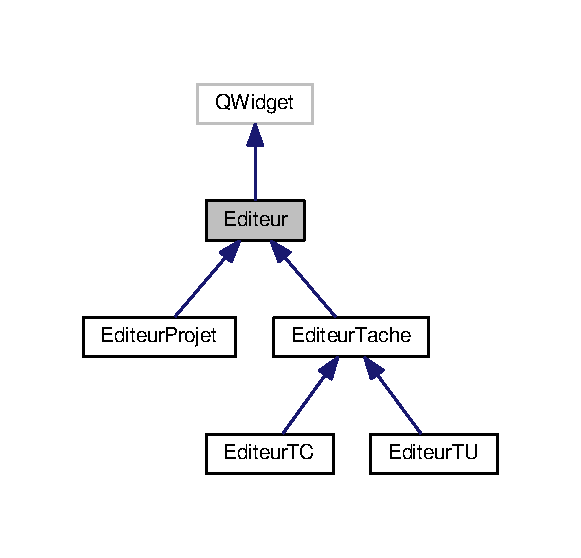
\includegraphics[width=279pt]{class_editeur__inherit__graph}
\end{center}
\end{figure}


Collaboration diagram for Editeur\+:\nopagebreak
\begin{figure}[H]
\begin{center}
\leavevmode
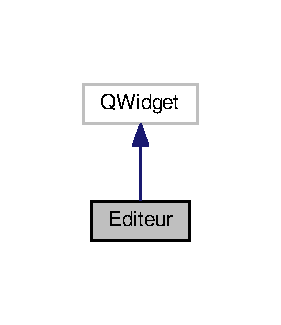
\includegraphics[width=135pt]{class_editeur__coll__graph}
\end{center}
\end{figure}
\subsection*{Public Slots}
\begin{DoxyCompactItemize}
\item 
virtual void \hyperlink{class_editeur_a1a3347bf7dbaeceff75c3e680538cac0}{slot\+Save} ()=0
\begin{DoxyCompactList}\small\item\em Fonction virtuelle pure dédiée à la sauvegarde de la tache ou du projet en cours d\textquotesingle{}édition. \end{DoxyCompactList}\item 
virtual void \hyperlink{class_editeur_ae2aaafb952d6c5a30e8ee07c68089ea4}{slot\+Reload} ()=0
\begin{DoxyCompactList}\small\item\em Fonction virtuelle pure remettant à zéro le formulaire d\textquotesingle{}édition. \end{DoxyCompactList}\end{DoxyCompactItemize}
\subsection*{Public Member Functions}
\begin{DoxyCompactItemize}
\item 
virtual \hyperlink{class_editeur_abebd575d846e6216a3380d36a98667fe}{$\sim$\+Editeur} ()
\item 
\hyperlink{class_editeur_a9bcddfc63dada09233c785674c995221}{Editeur} ()
\end{DoxyCompactItemize}
\subsection*{Public Attributes}
\begin{DoxyCompactItemize}
\item 
Q\+Form\+Layout $\ast$ \hyperlink{class_editeur_ab1c926cc589df5011910a45480bf08f0}{form\+Layout}
\end{DoxyCompactItemize}


\subsection{Detailed Description}
Classe abstraite pour le widget d\textquotesingle{}édition (partie droite de l\textquotesingle{}onglet d\textquotesingle{}édition) 

Contient le form\+Layout et des classes virtuelles pures d\textquotesingle{}enregistrement et de chargement des taches/projets. 

\subsection{Constructor \& Destructor Documentation}
\hypertarget{class_editeur_abebd575d846e6216a3380d36a98667fe}{}\index{Editeur@{Editeur}!````~Editeur@{$\sim$\+Editeur}}
\index{````~Editeur@{$\sim$\+Editeur}!Editeur@{Editeur}}
\subsubsection[{$\sim$\+Editeur}]{\setlength{\rightskip}{0pt plus 5cm}virtual Editeur\+::$\sim$\+Editeur (
\begin{DoxyParamCaption}
{}
\end{DoxyParamCaption}
)\hspace{0.3cm}{\ttfamily [inline]}, {\ttfamily [virtual]}}\label{class_editeur_abebd575d846e6216a3380d36a98667fe}
\hypertarget{class_editeur_a9bcddfc63dada09233c785674c995221}{}\index{Editeur@{Editeur}!Editeur@{Editeur}}
\index{Editeur@{Editeur}!Editeur@{Editeur}}
\subsubsection[{Editeur}]{\setlength{\rightskip}{0pt plus 5cm}Editeur\+::\+Editeur (
\begin{DoxyParamCaption}
{}
\end{DoxyParamCaption}
)\hspace{0.3cm}{\ttfamily [inline]}}\label{class_editeur_a9bcddfc63dada09233c785674c995221}


\subsection{Member Function Documentation}
\hypertarget{class_editeur_ae2aaafb952d6c5a30e8ee07c68089ea4}{}\index{Editeur@{Editeur}!slot\+Reload@{slot\+Reload}}
\index{slot\+Reload@{slot\+Reload}!Editeur@{Editeur}}
\subsubsection[{slot\+Reload}]{\setlength{\rightskip}{0pt plus 5cm}virtual void Editeur\+::slot\+Reload (
\begin{DoxyParamCaption}
{}
\end{DoxyParamCaption}
)\hspace{0.3cm}{\ttfamily [pure virtual]}, {\ttfamily [slot]}}\label{class_editeur_ae2aaafb952d6c5a30e8ee07c68089ea4}


Fonction virtuelle pure remettant à zéro le formulaire d\textquotesingle{}édition. 

\hypertarget{class_editeur_a1a3347bf7dbaeceff75c3e680538cac0}{}\index{Editeur@{Editeur}!slot\+Save@{slot\+Save}}
\index{slot\+Save@{slot\+Save}!Editeur@{Editeur}}
\subsubsection[{slot\+Save}]{\setlength{\rightskip}{0pt plus 5cm}virtual void Editeur\+::slot\+Save (
\begin{DoxyParamCaption}
{}
\end{DoxyParamCaption}
)\hspace{0.3cm}{\ttfamily [pure virtual]}, {\ttfamily [slot]}}\label{class_editeur_a1a3347bf7dbaeceff75c3e680538cac0}


Fonction virtuelle pure dédiée à la sauvegarde de la tache ou du projet en cours d\textquotesingle{}édition. 



\subsection{Member Data Documentation}
\hypertarget{class_editeur_ab1c926cc589df5011910a45480bf08f0}{}\index{Editeur@{Editeur}!form\+Layout@{form\+Layout}}
\index{form\+Layout@{form\+Layout}!Editeur@{Editeur}}
\subsubsection[{form\+Layout}]{\setlength{\rightskip}{0pt plus 5cm}Q\+Form\+Layout$\ast$ Editeur\+::form\+Layout}\label{class_editeur_ab1c926cc589df5011910a45480bf08f0}


The documentation for this class was generated from the following file\+:\begin{DoxyCompactItemize}
\item 
L\+O21app/\hyperlink{_u_i_classes_8h}{U\+I\+Classes.\+h}\end{DoxyCompactItemize}

\hypertarget{class_editeur_precedence}{}\section{Editeur\+Precedence Class Reference}
\label{class_editeur_precedence}\index{Editeur\+Precedence@{Editeur\+Precedence}}


\hyperlink{class_editeur}{Editeur} des précédences de la tache appelante.  




{\ttfamily \#include $<$U\+I\+Classes.\+h$>$}



Inheritance diagram for Editeur\+Precedence\+:\nopagebreak
\begin{figure}[H]
\begin{center}
\leavevmode
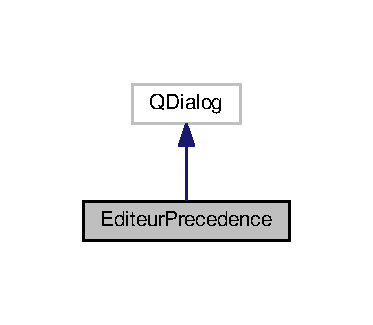
\includegraphics[width=179pt]{class_editeur_precedence__inherit__graph}
\end{center}
\end{figure}


Collaboration diagram for Editeur\+Precedence\+:\nopagebreak
\begin{figure}[H]
\begin{center}
\leavevmode
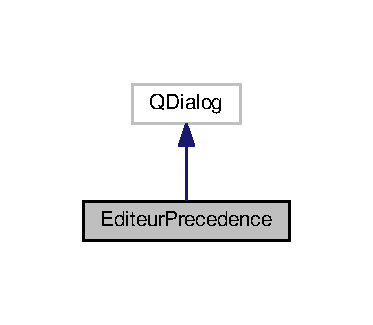
\includegraphics[width=179pt]{class_editeur_precedence__coll__graph}
\end{center}
\end{figure}
\subsection*{Public Slots}
\begin{DoxyCompactItemize}
\item 
void \hyperlink{class_editeur_precedence_a6553c232071fb5b260266f42ff68e034}{slot\+Annulation} ()
\begin{DoxyCompactList}\small\item\em Termine l\textquotesingle{}édition des précédences et ferme. \end{DoxyCompactList}\item 
void \hyperlink{class_editeur_precedence_a8afea493809dd7de5adf873cf53c2269}{slot\+Ajout} ()
\begin{DoxyCompactList}\small\item\em Ajoute la précédence et ferme le dialogue. \end{DoxyCompactList}\end{DoxyCompactItemize}
\subsection*{Signals}
\begin{DoxyCompactItemize}
\item 
void \hyperlink{class_editeur_precedence_abc08fe095980f3562b33d5d77db2b78c}{edition\+Precedence\+End} ()
\begin{DoxyCompactList}\small\item\em L\textquotesingle{}édition des précédences est terminée (validée ou annulée) \end{DoxyCompactList}\end{DoxyCompactItemize}
\subsection*{Public Member Functions}
\begin{DoxyCompactItemize}
\item 
\hyperlink{class_editeur_precedence_a60f724870e7782eb7173899301697de7}{Editeur\+Precedence} (\hyperlink{class_tache}{Tache} $\ast$t)
\item 
string \& \hyperlink{class_editeur_precedence_a4daa5c22356a9d1bd1dff590f8c48493}{get\+Tache\+Id\+From\+Index} (int index)
\begin{DoxyCompactList}\small\item\em Retourne l\textquotesingle{}id de la tache choisie dans la Combobox. \end{DoxyCompactList}\item 
bool \hyperlink{class_editeur_precedence_a23123b51c204c65e76950b3c5fa0145d}{empty} () const 
\begin{DoxyCompactList}\small\item\em Retourne true s\textquotesingle{}il n\textquotesingle{}y a pas de précédence possible (entraine la non ouverture du dialogue) \end{DoxyCompactList}\end{DoxyCompactItemize}


\subsection{Detailed Description}
\hyperlink{class_editeur}{Editeur} des précédences de la tache appelante. 

\subsection{Constructor \& Destructor Documentation}
\hypertarget{class_editeur_precedence_a60f724870e7782eb7173899301697de7}{}\index{Editeur\+Precedence@{Editeur\+Precedence}!Editeur\+Precedence@{Editeur\+Precedence}}
\index{Editeur\+Precedence@{Editeur\+Precedence}!Editeur\+Precedence@{Editeur\+Precedence}}
\subsubsection[{Editeur\+Precedence}]{\setlength{\rightskip}{0pt plus 5cm}Editeur\+Precedence\+::\+Editeur\+Precedence (
\begin{DoxyParamCaption}
\item[{{\bf Tache} $\ast$}]{t}
\end{DoxyParamCaption}
)}\label{class_editeur_precedence_a60f724870e7782eb7173899301697de7}


\subsection{Member Function Documentation}
\hypertarget{class_editeur_precedence_abc08fe095980f3562b33d5d77db2b78c}{}\index{Editeur\+Precedence@{Editeur\+Precedence}!edition\+Precedence\+End@{edition\+Precedence\+End}}
\index{edition\+Precedence\+End@{edition\+Precedence\+End}!Editeur\+Precedence@{Editeur\+Precedence}}
\subsubsection[{edition\+Precedence\+End}]{\setlength{\rightskip}{0pt plus 5cm}void Editeur\+Precedence\+::edition\+Precedence\+End (
\begin{DoxyParamCaption}
{}
\end{DoxyParamCaption}
)\hspace{0.3cm}{\ttfamily [signal]}}\label{class_editeur_precedence_abc08fe095980f3562b33d5d77db2b78c}


L\textquotesingle{}édition des précédences est terminée (validée ou annulée) 

\hypertarget{class_editeur_precedence_a23123b51c204c65e76950b3c5fa0145d}{}\index{Editeur\+Precedence@{Editeur\+Precedence}!empty@{empty}}
\index{empty@{empty}!Editeur\+Precedence@{Editeur\+Precedence}}
\subsubsection[{empty}]{\setlength{\rightskip}{0pt plus 5cm}bool Editeur\+Precedence\+::empty (
\begin{DoxyParamCaption}
{}
\end{DoxyParamCaption}
) const\hspace{0.3cm}{\ttfamily [inline]}}\label{class_editeur_precedence_a23123b51c204c65e76950b3c5fa0145d}


Retourne true s\textquotesingle{}il n\textquotesingle{}y a pas de précédence possible (entraine la non ouverture du dialogue) 

\hypertarget{class_editeur_precedence_a4daa5c22356a9d1bd1dff590f8c48493}{}\index{Editeur\+Precedence@{Editeur\+Precedence}!get\+Tache\+Id\+From\+Index@{get\+Tache\+Id\+From\+Index}}
\index{get\+Tache\+Id\+From\+Index@{get\+Tache\+Id\+From\+Index}!Editeur\+Precedence@{Editeur\+Precedence}}
\subsubsection[{get\+Tache\+Id\+From\+Index}]{\setlength{\rightskip}{0pt plus 5cm}string \& Editeur\+Precedence\+::get\+Tache\+Id\+From\+Index (
\begin{DoxyParamCaption}
\item[{int}]{index}
\end{DoxyParamCaption}
)}\label{class_editeur_precedence_a4daa5c22356a9d1bd1dff590f8c48493}


Retourne l\textquotesingle{}id de la tache choisie dans la Combobox. 

\hypertarget{class_editeur_precedence_a8afea493809dd7de5adf873cf53c2269}{}\index{Editeur\+Precedence@{Editeur\+Precedence}!slot\+Ajout@{slot\+Ajout}}
\index{slot\+Ajout@{slot\+Ajout}!Editeur\+Precedence@{Editeur\+Precedence}}
\subsubsection[{slot\+Ajout}]{\setlength{\rightskip}{0pt plus 5cm}void Editeur\+Precedence\+::slot\+Ajout (
\begin{DoxyParamCaption}
{}
\end{DoxyParamCaption}
)\hspace{0.3cm}{\ttfamily [slot]}}\label{class_editeur_precedence_a8afea493809dd7de5adf873cf53c2269}


Ajoute la précédence et ferme le dialogue. 

\hypertarget{class_editeur_precedence_a6553c232071fb5b260266f42ff68e034}{}\index{Editeur\+Precedence@{Editeur\+Precedence}!slot\+Annulation@{slot\+Annulation}}
\index{slot\+Annulation@{slot\+Annulation}!Editeur\+Precedence@{Editeur\+Precedence}}
\subsubsection[{slot\+Annulation}]{\setlength{\rightskip}{0pt plus 5cm}void Editeur\+Precedence\+::slot\+Annulation (
\begin{DoxyParamCaption}
{}
\end{DoxyParamCaption}
)\hspace{0.3cm}{\ttfamily [slot]}}\label{class_editeur_precedence_a6553c232071fb5b260266f42ff68e034}


Termine l\textquotesingle{}édition des précédences et ferme. 



The documentation for this class was generated from the following files\+:\begin{DoxyCompactItemize}
\item 
L\+O21app/\hyperlink{_u_i_classes_8h}{U\+I\+Classes.\+h}\item 
L\+O21app/\hyperlink{_u_i_classes_8cpp}{U\+I\+Classes.\+cpp}\end{DoxyCompactItemize}

\hypertarget{class_editeur_projet}{}\section{Editeur\+Projet Class Reference}
\label{class_editeur_projet}\index{Editeur\+Projet@{Editeur\+Projet}}


Classe pour l\textquotesingle{}\hyperlink{class_editeur}{Editeur} de projet.  




{\ttfamily \#include $<$U\+I\+Classes.\+h$>$}



Inheritance diagram for Editeur\+Projet\+:\nopagebreak
\begin{figure}[H]
\begin{center}
\leavevmode
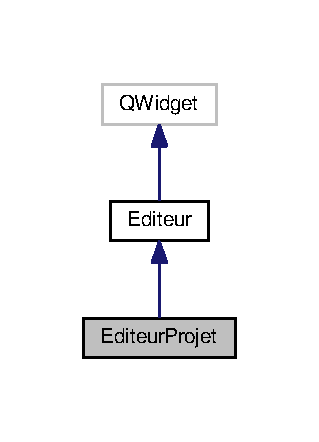
\includegraphics[width=153pt]{class_editeur_projet__inherit__graph}
\end{center}
\end{figure}


Collaboration diagram for Editeur\+Projet\+:\nopagebreak
\begin{figure}[H]
\begin{center}
\leavevmode
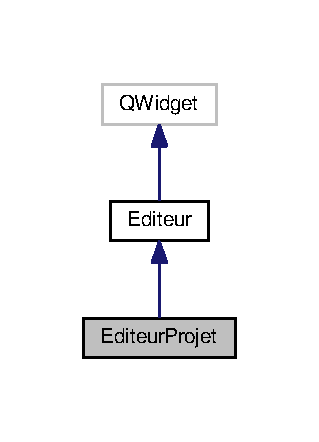
\includegraphics[width=153pt]{class_editeur_projet__coll__graph}
\end{center}
\end{figure}
\subsection*{Public Slots}
\begin{DoxyCompactItemize}
\item 
void \hyperlink{class_editeur_projet_a9982e3188058e70345faf052aedf6325}{slot\+Save} ()
\item 
void \hyperlink{class_editeur_projet_acb6efff25441f2b8f4c5507dc5b90cf5}{slot\+Exporter} ()
\begin{DoxyCompactList}\small\item\em Exporte le projet sous forme d\textquotesingle{}un fichier X\+M\+L. \end{DoxyCompactList}\item 
void \hyperlink{class_editeur_projet_a8a527a6cf36fe24036e47735ebadd735}{slot\+Reload} ()
\end{DoxyCompactItemize}
\subsection*{Signals}
\begin{DoxyCompactItemize}
\item 
void \hyperlink{class_editeur_projet_afcab9b5c1e80acfa8a33e1bf64bcf85f}{projet\+Updated} (\hyperlink{class_projet}{Projet} $\ast$projet)
\begin{DoxyCompactList}\small\item\em Le projet passé en paramètre a été modifié \end{DoxyCompactList}\end{DoxyCompactItemize}
\subsection*{Public Member Functions}
\begin{DoxyCompactItemize}
\item 
\hyperlink{class_editeur_projet_acde1e8bcea74603569215c0cd2331258}{Editeur\+Projet} (\hyperlink{class_projet}{Projet} $\ast$p)
\item 
virtual \hyperlink{class_editeur_projet_a5fb06458b4bd5d5df9d57915adb1e2ce}{$\sim$\+Editeur\+Projet} ()
\end{DoxyCompactItemize}
\subsection*{Additional Inherited Members}


\subsection{Detailed Description}
Classe pour l\textquotesingle{}\hyperlink{class_editeur}{Editeur} de projet. 

Remplit le formulaire, l\textquotesingle{}enregistre et l\textquotesingle{}exporte en X\+M\+L 

\subsection{Constructor \& Destructor Documentation}
\hypertarget{class_editeur_projet_acde1e8bcea74603569215c0cd2331258}{}\index{Editeur\+Projet@{Editeur\+Projet}!Editeur\+Projet@{Editeur\+Projet}}
\index{Editeur\+Projet@{Editeur\+Projet}!Editeur\+Projet@{Editeur\+Projet}}
\subsubsection[{Editeur\+Projet}]{\setlength{\rightskip}{0pt plus 5cm}Editeur\+Projet\+::\+Editeur\+Projet (
\begin{DoxyParamCaption}
\item[{{\bf Projet} $\ast$}]{p}
\end{DoxyParamCaption}
)}\label{class_editeur_projet_acde1e8bcea74603569215c0cd2331258}
\hypertarget{class_editeur_projet_a5fb06458b4bd5d5df9d57915adb1e2ce}{}\index{Editeur\+Projet@{Editeur\+Projet}!````~Editeur\+Projet@{$\sim$\+Editeur\+Projet}}
\index{````~Editeur\+Projet@{$\sim$\+Editeur\+Projet}!Editeur\+Projet@{Editeur\+Projet}}
\subsubsection[{$\sim$\+Editeur\+Projet}]{\setlength{\rightskip}{0pt plus 5cm}virtual Editeur\+Projet\+::$\sim$\+Editeur\+Projet (
\begin{DoxyParamCaption}
{}
\end{DoxyParamCaption}
)\hspace{0.3cm}{\ttfamily [inline]}, {\ttfamily [virtual]}}\label{class_editeur_projet_a5fb06458b4bd5d5df9d57915adb1e2ce}


\subsection{Member Function Documentation}
\hypertarget{class_editeur_projet_afcab9b5c1e80acfa8a33e1bf64bcf85f}{}\index{Editeur\+Projet@{Editeur\+Projet}!projet\+Updated@{projet\+Updated}}
\index{projet\+Updated@{projet\+Updated}!Editeur\+Projet@{Editeur\+Projet}}
\subsubsection[{projet\+Updated}]{\setlength{\rightskip}{0pt plus 5cm}void Editeur\+Projet\+::projet\+Updated (
\begin{DoxyParamCaption}
\item[{{\bf Projet} $\ast$}]{projet}
\end{DoxyParamCaption}
)\hspace{0.3cm}{\ttfamily [signal]}}\label{class_editeur_projet_afcab9b5c1e80acfa8a33e1bf64bcf85f}


Le projet passé en paramètre a été modifié 

\hypertarget{class_editeur_projet_acb6efff25441f2b8f4c5507dc5b90cf5}{}\index{Editeur\+Projet@{Editeur\+Projet}!slot\+Exporter@{slot\+Exporter}}
\index{slot\+Exporter@{slot\+Exporter}!Editeur\+Projet@{Editeur\+Projet}}
\subsubsection[{slot\+Exporter}]{\setlength{\rightskip}{0pt plus 5cm}void Editeur\+Projet\+::slot\+Exporter (
\begin{DoxyParamCaption}
{}
\end{DoxyParamCaption}
)\hspace{0.3cm}{\ttfamily [slot]}}\label{class_editeur_projet_acb6efff25441f2b8f4c5507dc5b90cf5}


Exporte le projet sous forme d\textquotesingle{}un fichier X\+M\+L. 

\hypertarget{class_editeur_projet_a8a527a6cf36fe24036e47735ebadd735}{}\index{Editeur\+Projet@{Editeur\+Projet}!slot\+Reload@{slot\+Reload}}
\index{slot\+Reload@{slot\+Reload}!Editeur\+Projet@{Editeur\+Projet}}
\subsubsection[{slot\+Reload}]{\setlength{\rightskip}{0pt plus 5cm}void Editeur\+Projet\+::slot\+Reload (
\begin{DoxyParamCaption}
{}
\end{DoxyParamCaption}
)\hspace{0.3cm}{\ttfamily [slot]}}\label{class_editeur_projet_a8a527a6cf36fe24036e47735ebadd735}
\hypertarget{class_editeur_projet_a9982e3188058e70345faf052aedf6325}{}\index{Editeur\+Projet@{Editeur\+Projet}!slot\+Save@{slot\+Save}}
\index{slot\+Save@{slot\+Save}!Editeur\+Projet@{Editeur\+Projet}}
\subsubsection[{slot\+Save}]{\setlength{\rightskip}{0pt plus 5cm}void Editeur\+Projet\+::slot\+Save (
\begin{DoxyParamCaption}
{}
\end{DoxyParamCaption}
)\hspace{0.3cm}{\ttfamily [slot]}}\label{class_editeur_projet_a9982e3188058e70345faf052aedf6325}


The documentation for this class was generated from the following files\+:\begin{DoxyCompactItemize}
\item 
L\+O21app/\hyperlink{_u_i_classes_8h}{U\+I\+Classes.\+h}\item 
L\+O21app/\hyperlink{_u_i_classes_8cpp}{U\+I\+Classes.\+cpp}\end{DoxyCompactItemize}

\hypertarget{class_editeur_tache}{}\section{Editeur\+Tache Class Reference}
\label{class_editeur_tache}\index{Editeur\+Tache@{Editeur\+Tache}}


Classe abstraite pour l\textquotesingle{}\hyperlink{class_editeur}{Editeur} de taches.  




{\ttfamily \#include $<$U\+I\+Classes.\+h$>$}



Inheritance diagram for Editeur\+Tache\+:\nopagebreak
\begin{figure}[H]
\begin{center}
\leavevmode
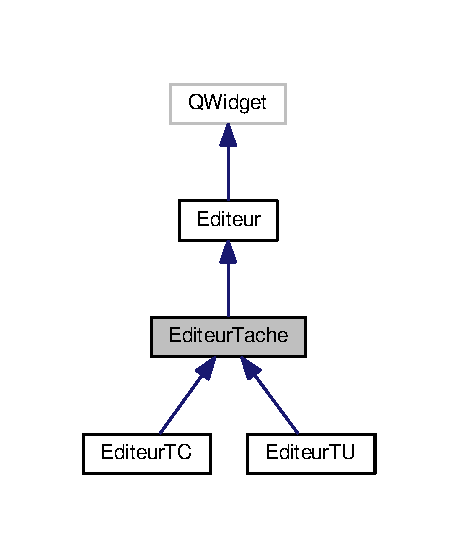
\includegraphics[width=220pt]{class_editeur_tache__inherit__graph}
\end{center}
\end{figure}


Collaboration diagram for Editeur\+Tache\+:\nopagebreak
\begin{figure}[H]
\begin{center}
\leavevmode
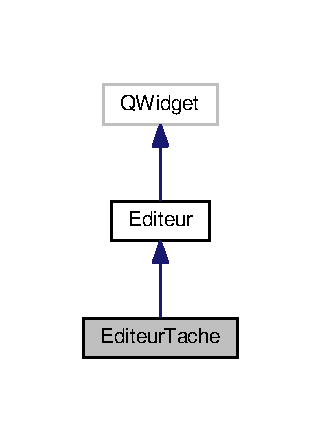
\includegraphics[width=154pt]{class_editeur_tache__coll__graph}
\end{center}
\end{figure}
\subsection*{Public Slots}
\begin{DoxyCompactItemize}
\item 
void \hyperlink{class_editeur_tache_a3da47f10289e4a6d06a758e15b9cf75b}{slot\+Enable} ()
\begin{DoxyCompactList}\small\item\em Active le widget. \end{DoxyCompactList}\item 
virtual void \hyperlink{class_editeur_tache_a74d5b6312857eb3eb906d91e62120117}{slot\+Reload} ()=0
\end{DoxyCompactItemize}
\subsection*{Signals}
\begin{DoxyCompactItemize}
\item 
void \hyperlink{class_editeur_tache_adf24ca27b5a0b0280b83c3f73d4e6bfa}{reload\+All} ()
\begin{DoxyCompactList}\small\item\em Demande d\textquotesingle{}actualisation du widget d\textquotesingle{}édition. \end{DoxyCompactList}\end{DoxyCompactItemize}
\subsection*{Public Member Functions}
\begin{DoxyCompactItemize}
\item 
\hyperlink{class_editeur_tache_af009a1d4c96dab70e199d53060f039e0}{Editeur\+Tache} ()
\item 
void \hyperlink{class_editeur_tache_a6f5dab1963119064dc44f0ec27dd2d59}{print\+Fin\+Form} (\hyperlink{class_tache}{Tache} $\ast$t)
\begin{DoxyCompactList}\small\item\em Affiche la fin du formulaire d\textquotesingle{}édition de tache, qui est commun aux unitaires et composites. \end{DoxyCompactList}\item 
virtual \hyperlink{class_editeur_tache_a68ce9a1be85d6ed5f27414fbc776080b}{$\sim$\+Editeur\+Tache} ()
\end{DoxyCompactItemize}
\subsection*{Public Attributes}
\begin{DoxyCompactItemize}
\item 
Q\+Line\+Edit $\ast$ \hyperlink{class_editeur_tache_a188e190433234ece59f36b9f633013da}{titre}
\item 
Q\+Calendar\+Widget $\ast$ \hyperlink{class_editeur_tache_a7a608a687eb98bf443067908744b3f94}{dispo}
\item 
Q\+Calendar\+Widget $\ast$ \hyperlink{class_editeur_tache_a93278524e408b25fec5671a6d1266fe1}{echeance}
\item 
Q\+Push\+Button $\ast$ \hyperlink{class_editeur_tache_ab6339fa7828a4dabf8f126f1d09661ff}{annuler}
\item 
Q\+Push\+Button $\ast$ \hyperlink{class_editeur_tache_a4b5c16b951e61f07047bd7ee4bf6d026}{sauver}
\item 
Q\+Push\+Button $\ast$ \hyperlink{class_editeur_tache_a18dc840a560062902f3cc5e382c03d6f}{predecesseurs}
\item 
Q\+List\+Widget $\ast$ \hyperlink{class_editeur_tache_ab16d5f996e09c161b95952f3e868a9f5}{liste\+Predecesseurs}
\item 
Q\+List\+Widget\+Item $\ast$$\ast$ \hyperlink{class_editeur_tache_ac5571067515d4f44d85d206b4e68ffc2}{tab\+Predecesseurs}
\item 
int \hyperlink{class_editeur_tache_acfe4d83f7a169b6f537e36876ec1ce84}{nb\+Pred}
\end{DoxyCompactItemize}


\subsection{Detailed Description}
Classe abstraite pour l\textquotesingle{}\hyperlink{class_editeur}{Editeur} de taches. 

\subsection{Constructor \& Destructor Documentation}
\hypertarget{class_editeur_tache_af009a1d4c96dab70e199d53060f039e0}{}\index{Editeur\+Tache@{Editeur\+Tache}!Editeur\+Tache@{Editeur\+Tache}}
\index{Editeur\+Tache@{Editeur\+Tache}!Editeur\+Tache@{Editeur\+Tache}}
\subsubsection[{Editeur\+Tache}]{\setlength{\rightskip}{0pt plus 5cm}Editeur\+Tache\+::\+Editeur\+Tache (
\begin{DoxyParamCaption}
{}
\end{DoxyParamCaption}
)}\label{class_editeur_tache_af009a1d4c96dab70e199d53060f039e0}
\hypertarget{class_editeur_tache_a68ce9a1be85d6ed5f27414fbc776080b}{}\index{Editeur\+Tache@{Editeur\+Tache}!````~Editeur\+Tache@{$\sim$\+Editeur\+Tache}}
\index{````~Editeur\+Tache@{$\sim$\+Editeur\+Tache}!Editeur\+Tache@{Editeur\+Tache}}
\subsubsection[{$\sim$\+Editeur\+Tache}]{\setlength{\rightskip}{0pt plus 5cm}virtual Editeur\+Tache\+::$\sim$\+Editeur\+Tache (
\begin{DoxyParamCaption}
{}
\end{DoxyParamCaption}
)\hspace{0.3cm}{\ttfamily [inline]}, {\ttfamily [virtual]}}\label{class_editeur_tache_a68ce9a1be85d6ed5f27414fbc776080b}


\subsection{Member Function Documentation}
\hypertarget{class_editeur_tache_a6f5dab1963119064dc44f0ec27dd2d59}{}\index{Editeur\+Tache@{Editeur\+Tache}!print\+Fin\+Form@{print\+Fin\+Form}}
\index{print\+Fin\+Form@{print\+Fin\+Form}!Editeur\+Tache@{Editeur\+Tache}}
\subsubsection[{print\+Fin\+Form}]{\setlength{\rightskip}{0pt plus 5cm}void Editeur\+Tache\+::print\+Fin\+Form (
\begin{DoxyParamCaption}
\item[{{\bf Tache} $\ast$}]{t}
\end{DoxyParamCaption}
)}\label{class_editeur_tache_a6f5dab1963119064dc44f0ec27dd2d59}


Affiche la fin du formulaire d\textquotesingle{}édition de tache, qui est commun aux unitaires et composites. 

\hypertarget{class_editeur_tache_adf24ca27b5a0b0280b83c3f73d4e6bfa}{}\index{Editeur\+Tache@{Editeur\+Tache}!reload\+All@{reload\+All}}
\index{reload\+All@{reload\+All}!Editeur\+Tache@{Editeur\+Tache}}
\subsubsection[{reload\+All}]{\setlength{\rightskip}{0pt plus 5cm}void Editeur\+Tache\+::reload\+All (
\begin{DoxyParamCaption}
{}
\end{DoxyParamCaption}
)\hspace{0.3cm}{\ttfamily [signal]}}\label{class_editeur_tache_adf24ca27b5a0b0280b83c3f73d4e6bfa}


Demande d\textquotesingle{}actualisation du widget d\textquotesingle{}édition. 

\hypertarget{class_editeur_tache_a3da47f10289e4a6d06a758e15b9cf75b}{}\index{Editeur\+Tache@{Editeur\+Tache}!slot\+Enable@{slot\+Enable}}
\index{slot\+Enable@{slot\+Enable}!Editeur\+Tache@{Editeur\+Tache}}
\subsubsection[{slot\+Enable}]{\setlength{\rightskip}{0pt plus 5cm}void Editeur\+Tache\+::slot\+Enable (
\begin{DoxyParamCaption}
{}
\end{DoxyParamCaption}
)\hspace{0.3cm}{\ttfamily [slot]}}\label{class_editeur_tache_a3da47f10289e4a6d06a758e15b9cf75b}


Active le widget. 

\hypertarget{class_editeur_tache_a74d5b6312857eb3eb906d91e62120117}{}\index{Editeur\+Tache@{Editeur\+Tache}!slot\+Reload@{slot\+Reload}}
\index{slot\+Reload@{slot\+Reload}!Editeur\+Tache@{Editeur\+Tache}}
\subsubsection[{slot\+Reload}]{\setlength{\rightskip}{0pt plus 5cm}virtual void Editeur\+Tache\+::slot\+Reload (
\begin{DoxyParamCaption}
{}
\end{DoxyParamCaption}
)\hspace{0.3cm}{\ttfamily [pure virtual]}, {\ttfamily [slot]}}\label{class_editeur_tache_a74d5b6312857eb3eb906d91e62120117}


\subsection{Member Data Documentation}
\hypertarget{class_editeur_tache_ab6339fa7828a4dabf8f126f1d09661ff}{}\index{Editeur\+Tache@{Editeur\+Tache}!annuler@{annuler}}
\index{annuler@{annuler}!Editeur\+Tache@{Editeur\+Tache}}
\subsubsection[{annuler}]{\setlength{\rightskip}{0pt plus 5cm}Q\+Push\+Button$\ast$ Editeur\+Tache\+::annuler}\label{class_editeur_tache_ab6339fa7828a4dabf8f126f1d09661ff}
\hypertarget{class_editeur_tache_a7a608a687eb98bf443067908744b3f94}{}\index{Editeur\+Tache@{Editeur\+Tache}!dispo@{dispo}}
\index{dispo@{dispo}!Editeur\+Tache@{Editeur\+Tache}}
\subsubsection[{dispo}]{\setlength{\rightskip}{0pt plus 5cm}Q\+Calendar\+Widget$\ast$ Editeur\+Tache\+::dispo}\label{class_editeur_tache_a7a608a687eb98bf443067908744b3f94}
\hypertarget{class_editeur_tache_a93278524e408b25fec5671a6d1266fe1}{}\index{Editeur\+Tache@{Editeur\+Tache}!echeance@{echeance}}
\index{echeance@{echeance}!Editeur\+Tache@{Editeur\+Tache}}
\subsubsection[{echeance}]{\setlength{\rightskip}{0pt plus 5cm}Q\+Calendar\+Widget$\ast$ Editeur\+Tache\+::echeance}\label{class_editeur_tache_a93278524e408b25fec5671a6d1266fe1}
\hypertarget{class_editeur_tache_ab16d5f996e09c161b95952f3e868a9f5}{}\index{Editeur\+Tache@{Editeur\+Tache}!liste\+Predecesseurs@{liste\+Predecesseurs}}
\index{liste\+Predecesseurs@{liste\+Predecesseurs}!Editeur\+Tache@{Editeur\+Tache}}
\subsubsection[{liste\+Predecesseurs}]{\setlength{\rightskip}{0pt plus 5cm}Q\+List\+Widget$\ast$ Editeur\+Tache\+::liste\+Predecesseurs}\label{class_editeur_tache_ab16d5f996e09c161b95952f3e868a9f5}
\hypertarget{class_editeur_tache_acfe4d83f7a169b6f537e36876ec1ce84}{}\index{Editeur\+Tache@{Editeur\+Tache}!nb\+Pred@{nb\+Pred}}
\index{nb\+Pred@{nb\+Pred}!Editeur\+Tache@{Editeur\+Tache}}
\subsubsection[{nb\+Pred}]{\setlength{\rightskip}{0pt plus 5cm}int Editeur\+Tache\+::nb\+Pred}\label{class_editeur_tache_acfe4d83f7a169b6f537e36876ec1ce84}
\hypertarget{class_editeur_tache_a18dc840a560062902f3cc5e382c03d6f}{}\index{Editeur\+Tache@{Editeur\+Tache}!predecesseurs@{predecesseurs}}
\index{predecesseurs@{predecesseurs}!Editeur\+Tache@{Editeur\+Tache}}
\subsubsection[{predecesseurs}]{\setlength{\rightskip}{0pt plus 5cm}Q\+Push\+Button$\ast$ Editeur\+Tache\+::predecesseurs}\label{class_editeur_tache_a18dc840a560062902f3cc5e382c03d6f}
\hypertarget{class_editeur_tache_a4b5c16b951e61f07047bd7ee4bf6d026}{}\index{Editeur\+Tache@{Editeur\+Tache}!sauver@{sauver}}
\index{sauver@{sauver}!Editeur\+Tache@{Editeur\+Tache}}
\subsubsection[{sauver}]{\setlength{\rightskip}{0pt plus 5cm}Q\+Push\+Button$\ast$ Editeur\+Tache\+::sauver}\label{class_editeur_tache_a4b5c16b951e61f07047bd7ee4bf6d026}
\hypertarget{class_editeur_tache_ac5571067515d4f44d85d206b4e68ffc2}{}\index{Editeur\+Tache@{Editeur\+Tache}!tab\+Predecesseurs@{tab\+Predecesseurs}}
\index{tab\+Predecesseurs@{tab\+Predecesseurs}!Editeur\+Tache@{Editeur\+Tache}}
\subsubsection[{tab\+Predecesseurs}]{\setlength{\rightskip}{0pt plus 5cm}Q\+List\+Widget\+Item$\ast$$\ast$ Editeur\+Tache\+::tab\+Predecesseurs}\label{class_editeur_tache_ac5571067515d4f44d85d206b4e68ffc2}
\hypertarget{class_editeur_tache_a188e190433234ece59f36b9f633013da}{}\index{Editeur\+Tache@{Editeur\+Tache}!titre@{titre}}
\index{titre@{titre}!Editeur\+Tache@{Editeur\+Tache}}
\subsubsection[{titre}]{\setlength{\rightskip}{0pt plus 5cm}Q\+Line\+Edit$\ast$ Editeur\+Tache\+::titre}\label{class_editeur_tache_a188e190433234ece59f36b9f633013da}


The documentation for this class was generated from the following files\+:\begin{DoxyCompactItemize}
\item 
L\+O21app/\hyperlink{_u_i_classes_8h}{U\+I\+Classes.\+h}\item 
L\+O21app/\hyperlink{_u_i_classes_8cpp}{U\+I\+Classes.\+cpp}\end{DoxyCompactItemize}

\hypertarget{class_editeur_t_c}{}\section{Editeur\+T\+C Class Reference}
\label{class_editeur_t_c}\index{Editeur\+T\+C@{Editeur\+T\+C}}


\hyperlink{class_editeur_tache}{Editeur\+Tache} de taches composite.  




{\ttfamily \#include $<$U\+I\+Classes.\+h$>$}



Inheritance diagram for Editeur\+T\+C\+:\nopagebreak
\begin{figure}[H]
\begin{center}
\leavevmode
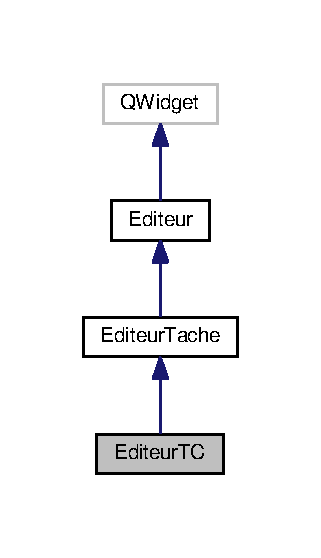
\includegraphics[width=154pt]{class_editeur_t_c__inherit__graph}
\end{center}
\end{figure}


Collaboration diagram for Editeur\+T\+C\+:\nopagebreak
\begin{figure}[H]
\begin{center}
\leavevmode
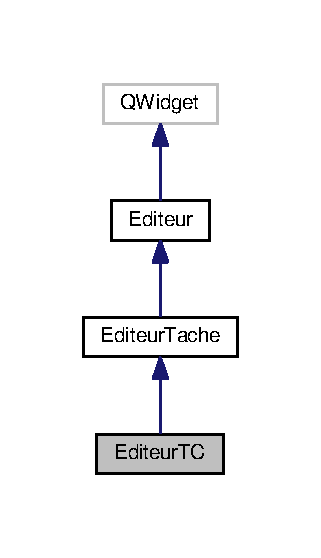
\includegraphics[width=154pt]{class_editeur_t_c__coll__graph}
\end{center}
\end{figure}
\subsection*{Public Slots}
\begin{DoxyCompactItemize}
\item 
void \hyperlink{class_editeur_t_c_a78904fa61e51fbd485aa792237285f99}{slot\+Save} ()
\item 
void \hyperlink{class_editeur_t_c_ad11356d9824f4cab16274988b2881c22}{slot\+Reload} ()
\item 
void \hyperlink{class_editeur_t_c_ab364f1db3119693a9af4785af0e156d6}{slot\+Edition\+Predecesseurs} ()
\begin{DoxyCompactList}\small\item\em Edite les préférences de la tache composite actuelle. \end{DoxyCompactList}\end{DoxyCompactItemize}
\subsection*{Signals}
\begin{DoxyCompactItemize}
\item 
void \hyperlink{class_editeur_t_c_a6bf8df2c0f505ce09faf9152a3fd1483}{tache\+Updated} (\hyperlink{class_composite}{Composite} $\ast$tache)
\begin{DoxyCompactList}\small\item\em Une tache composite vient d\textquotesingle{}etre éditée. \end{DoxyCompactList}\end{DoxyCompactItemize}
\subsection*{Public Member Functions}
\begin{DoxyCompactItemize}
\item 
virtual \hyperlink{class_editeur_t_c_a6cd28fad391d71dbdecec70ccc1cdf4f}{$\sim$\+Editeur\+T\+C} ()
\item 
\hyperlink{class_editeur_t_c_ac63bdb73f54321eda4d4cfea03f88df1}{Editeur\+T\+C} (\hyperlink{class_composite}{Composite} $\ast$t)
\end{DoxyCompactItemize}
\subsection*{Additional Inherited Members}


\subsection{Detailed Description}
\hyperlink{class_editeur_tache}{Editeur\+Tache} de taches composite. 

\subsection{Constructor \& Destructor Documentation}
\hypertarget{class_editeur_t_c_a6cd28fad391d71dbdecec70ccc1cdf4f}{}\index{Editeur\+T\+C@{Editeur\+T\+C}!````~Editeur\+T\+C@{$\sim$\+Editeur\+T\+C}}
\index{````~Editeur\+T\+C@{$\sim$\+Editeur\+T\+C}!Editeur\+T\+C@{Editeur\+T\+C}}
\subsubsection[{$\sim$\+Editeur\+T\+C}]{\setlength{\rightskip}{0pt plus 5cm}virtual Editeur\+T\+C\+::$\sim$\+Editeur\+T\+C (
\begin{DoxyParamCaption}
{}
\end{DoxyParamCaption}
)\hspace{0.3cm}{\ttfamily [inline]}, {\ttfamily [virtual]}}\label{class_editeur_t_c_a6cd28fad391d71dbdecec70ccc1cdf4f}
\hypertarget{class_editeur_t_c_ac63bdb73f54321eda4d4cfea03f88df1}{}\index{Editeur\+T\+C@{Editeur\+T\+C}!Editeur\+T\+C@{Editeur\+T\+C}}
\index{Editeur\+T\+C@{Editeur\+T\+C}!Editeur\+T\+C@{Editeur\+T\+C}}
\subsubsection[{Editeur\+T\+C}]{\setlength{\rightskip}{0pt plus 5cm}Editeur\+T\+C\+::\+Editeur\+T\+C (
\begin{DoxyParamCaption}
\item[{{\bf Composite} $\ast$}]{t}
\end{DoxyParamCaption}
)}\label{class_editeur_t_c_ac63bdb73f54321eda4d4cfea03f88df1}


\subsection{Member Function Documentation}
\hypertarget{class_editeur_t_c_ab364f1db3119693a9af4785af0e156d6}{}\index{Editeur\+T\+C@{Editeur\+T\+C}!slot\+Edition\+Predecesseurs@{slot\+Edition\+Predecesseurs}}
\index{slot\+Edition\+Predecesseurs@{slot\+Edition\+Predecesseurs}!Editeur\+T\+C@{Editeur\+T\+C}}
\subsubsection[{slot\+Edition\+Predecesseurs}]{\setlength{\rightskip}{0pt plus 5cm}void Editeur\+T\+C\+::slot\+Edition\+Predecesseurs (
\begin{DoxyParamCaption}
{}
\end{DoxyParamCaption}
)\hspace{0.3cm}{\ttfamily [slot]}}\label{class_editeur_t_c_ab364f1db3119693a9af4785af0e156d6}


Edite les préférences de la tache composite actuelle. 

\hypertarget{class_editeur_t_c_ad11356d9824f4cab16274988b2881c22}{}\index{Editeur\+T\+C@{Editeur\+T\+C}!slot\+Reload@{slot\+Reload}}
\index{slot\+Reload@{slot\+Reload}!Editeur\+T\+C@{Editeur\+T\+C}}
\subsubsection[{slot\+Reload}]{\setlength{\rightskip}{0pt plus 5cm}void Editeur\+T\+C\+::slot\+Reload (
\begin{DoxyParamCaption}
{}
\end{DoxyParamCaption}
)\hspace{0.3cm}{\ttfamily [slot]}}\label{class_editeur_t_c_ad11356d9824f4cab16274988b2881c22}
\hypertarget{class_editeur_t_c_a78904fa61e51fbd485aa792237285f99}{}\index{Editeur\+T\+C@{Editeur\+T\+C}!slot\+Save@{slot\+Save}}
\index{slot\+Save@{slot\+Save}!Editeur\+T\+C@{Editeur\+T\+C}}
\subsubsection[{slot\+Save}]{\setlength{\rightskip}{0pt plus 5cm}void Editeur\+T\+C\+::slot\+Save (
\begin{DoxyParamCaption}
{}
\end{DoxyParamCaption}
)\hspace{0.3cm}{\ttfamily [slot]}}\label{class_editeur_t_c_a78904fa61e51fbd485aa792237285f99}
\hypertarget{class_editeur_t_c_a6bf8df2c0f505ce09faf9152a3fd1483}{}\index{Editeur\+T\+C@{Editeur\+T\+C}!tache\+Updated@{tache\+Updated}}
\index{tache\+Updated@{tache\+Updated}!Editeur\+T\+C@{Editeur\+T\+C}}
\subsubsection[{tache\+Updated}]{\setlength{\rightskip}{0pt plus 5cm}void Editeur\+T\+C\+::tache\+Updated (
\begin{DoxyParamCaption}
\item[{{\bf Composite} $\ast$}]{tache}
\end{DoxyParamCaption}
)\hspace{0.3cm}{\ttfamily [signal]}}\label{class_editeur_t_c_a6bf8df2c0f505ce09faf9152a3fd1483}


Une tache composite vient d\textquotesingle{}etre éditée. 



The documentation for this class was generated from the following files\+:\begin{DoxyCompactItemize}
\item 
L\+O21app/\hyperlink{_u_i_classes_8h}{U\+I\+Classes.\+h}\item 
L\+O21app/\hyperlink{_u_i_classes_8cpp}{U\+I\+Classes.\+cpp}\end{DoxyCompactItemize}

\hypertarget{class_editeur_t_u}{}\section{Editeur\+T\+U Class Reference}
\label{class_editeur_t_u}\index{Editeur\+T\+U@{Editeur\+T\+U}}


\hyperlink{class_editeur_tache}{Editeur\+Tache} de taches unitaires.  




{\ttfamily \#include $<$U\+I\+Classes.\+h$>$}



Inheritance diagram for Editeur\+T\+U\+:\nopagebreak
\begin{figure}[H]
\begin{center}
\leavevmode
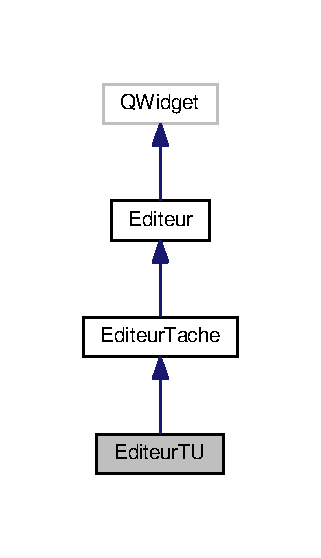
\includegraphics[width=154pt]{class_editeur_t_u__inherit__graph}
\end{center}
\end{figure}


Collaboration diagram for Editeur\+T\+U\+:\nopagebreak
\begin{figure}[H]
\begin{center}
\leavevmode
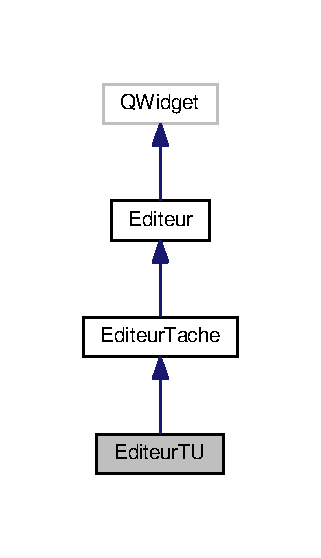
\includegraphics[width=154pt]{class_editeur_t_u__coll__graph}
\end{center}
\end{figure}
\subsection*{Public Slots}
\begin{DoxyCompactItemize}
\item 
void \hyperlink{class_editeur_t_u_a984d437115865a68627399a46044498b}{slot\+Save} ()
\item 
void \hyperlink{class_editeur_t_u_a13ca89536b3639d1a4e02b344dc94bac}{slot\+Reload} ()
\item 
void \hyperlink{class_editeur_t_u_a3d2a510d3b85a8c4faa6138a3652bedf}{slot\+Edition\+Predecesseurs} ()
\begin{DoxyCompactList}\small\item\em Edite les prédécesseurs de la tache unitaire actuelle. \end{DoxyCompactList}\end{DoxyCompactItemize}
\subsection*{Signals}
\begin{DoxyCompactItemize}
\item 
void \hyperlink{class_editeur_t_u_a274d794e10771caa0ae7f0078ef7123a}{tache\+Updated} (\hyperlink{class_unitaire}{Unitaire} $\ast$tache)
\begin{DoxyCompactList}\small\item\em Une tache unitaire vient d\textquotesingle{}etre éditée. \end{DoxyCompactList}\end{DoxyCompactItemize}
\subsection*{Public Member Functions}
\begin{DoxyCompactItemize}
\item 
virtual \hyperlink{class_editeur_t_u_a211cf15b8ca469ebc116e65047d520d7}{$\sim$\+Editeur\+T\+U} ()
\item 
\hyperlink{class_editeur_t_u_ae4ba80d6b96a46a51b2549e607cde008}{Editeur\+T\+U} (\hyperlink{class_unitaire}{Unitaire} $\ast$t)
\end{DoxyCompactItemize}
\subsection*{Additional Inherited Members}


\subsection{Detailed Description}
\hyperlink{class_editeur_tache}{Editeur\+Tache} de taches unitaires. 

\subsection{Constructor \& Destructor Documentation}
\hypertarget{class_editeur_t_u_a211cf15b8ca469ebc116e65047d520d7}{}\index{Editeur\+T\+U@{Editeur\+T\+U}!````~Editeur\+T\+U@{$\sim$\+Editeur\+T\+U}}
\index{````~Editeur\+T\+U@{$\sim$\+Editeur\+T\+U}!Editeur\+T\+U@{Editeur\+T\+U}}
\subsubsection[{$\sim$\+Editeur\+T\+U}]{\setlength{\rightskip}{0pt plus 5cm}virtual Editeur\+T\+U\+::$\sim$\+Editeur\+T\+U (
\begin{DoxyParamCaption}
{}
\end{DoxyParamCaption}
)\hspace{0.3cm}{\ttfamily [inline]}, {\ttfamily [virtual]}}\label{class_editeur_t_u_a211cf15b8ca469ebc116e65047d520d7}
\hypertarget{class_editeur_t_u_ae4ba80d6b96a46a51b2549e607cde008}{}\index{Editeur\+T\+U@{Editeur\+T\+U}!Editeur\+T\+U@{Editeur\+T\+U}}
\index{Editeur\+T\+U@{Editeur\+T\+U}!Editeur\+T\+U@{Editeur\+T\+U}}
\subsubsection[{Editeur\+T\+U}]{\setlength{\rightskip}{0pt plus 5cm}Editeur\+T\+U\+::\+Editeur\+T\+U (
\begin{DoxyParamCaption}
\item[{{\bf Unitaire} $\ast$}]{t}
\end{DoxyParamCaption}
)}\label{class_editeur_t_u_ae4ba80d6b96a46a51b2549e607cde008}


\subsection{Member Function Documentation}
\hypertarget{class_editeur_t_u_a3d2a510d3b85a8c4faa6138a3652bedf}{}\index{Editeur\+T\+U@{Editeur\+T\+U}!slot\+Edition\+Predecesseurs@{slot\+Edition\+Predecesseurs}}
\index{slot\+Edition\+Predecesseurs@{slot\+Edition\+Predecesseurs}!Editeur\+T\+U@{Editeur\+T\+U}}
\subsubsection[{slot\+Edition\+Predecesseurs}]{\setlength{\rightskip}{0pt plus 5cm}void Editeur\+T\+U\+::slot\+Edition\+Predecesseurs (
\begin{DoxyParamCaption}
{}
\end{DoxyParamCaption}
)\hspace{0.3cm}{\ttfamily [slot]}}\label{class_editeur_t_u_a3d2a510d3b85a8c4faa6138a3652bedf}


Edite les prédécesseurs de la tache unitaire actuelle. 

\hypertarget{class_editeur_t_u_a13ca89536b3639d1a4e02b344dc94bac}{}\index{Editeur\+T\+U@{Editeur\+T\+U}!slot\+Reload@{slot\+Reload}}
\index{slot\+Reload@{slot\+Reload}!Editeur\+T\+U@{Editeur\+T\+U}}
\subsubsection[{slot\+Reload}]{\setlength{\rightskip}{0pt plus 5cm}void Editeur\+T\+U\+::slot\+Reload (
\begin{DoxyParamCaption}
{}
\end{DoxyParamCaption}
)\hspace{0.3cm}{\ttfamily [slot]}}\label{class_editeur_t_u_a13ca89536b3639d1a4e02b344dc94bac}
\hypertarget{class_editeur_t_u_a984d437115865a68627399a46044498b}{}\index{Editeur\+T\+U@{Editeur\+T\+U}!slot\+Save@{slot\+Save}}
\index{slot\+Save@{slot\+Save}!Editeur\+T\+U@{Editeur\+T\+U}}
\subsubsection[{slot\+Save}]{\setlength{\rightskip}{0pt plus 5cm}void Editeur\+T\+U\+::slot\+Save (
\begin{DoxyParamCaption}
{}
\end{DoxyParamCaption}
)\hspace{0.3cm}{\ttfamily [slot]}}\label{class_editeur_t_u_a984d437115865a68627399a46044498b}
\hypertarget{class_editeur_t_u_a274d794e10771caa0ae7f0078ef7123a}{}\index{Editeur\+T\+U@{Editeur\+T\+U}!tache\+Updated@{tache\+Updated}}
\index{tache\+Updated@{tache\+Updated}!Editeur\+T\+U@{Editeur\+T\+U}}
\subsubsection[{tache\+Updated}]{\setlength{\rightskip}{0pt plus 5cm}void Editeur\+T\+U\+::tache\+Updated (
\begin{DoxyParamCaption}
\item[{{\bf Unitaire} $\ast$}]{tache}
\end{DoxyParamCaption}
)\hspace{0.3cm}{\ttfamily [signal]}}\label{class_editeur_t_u_a274d794e10771caa0ae7f0078ef7123a}


Une tache unitaire vient d\textquotesingle{}etre éditée. 



The documentation for this class was generated from the following files\+:\begin{DoxyCompactItemize}
\item 
L\+O21app/\hyperlink{_u_i_classes_8h}{U\+I\+Classes.\+h}\item 
L\+O21app/\hyperlink{_u_i_classes_8cpp}{U\+I\+Classes.\+cpp}\end{DoxyCompactItemize}

\hypertarget{class_evenement}{}\section{Evenement Class Reference}
\label{class_evenement}\index{Evenement@{Evenement}}


Classe abstraite d\textquotesingle{}éléments pouvant être programmés.  




{\ttfamily \#include $<$Calendar.\+h$>$}



Inheritance diagram for Evenement\+:\nopagebreak
\begin{figure}[H]
\begin{center}
\leavevmode
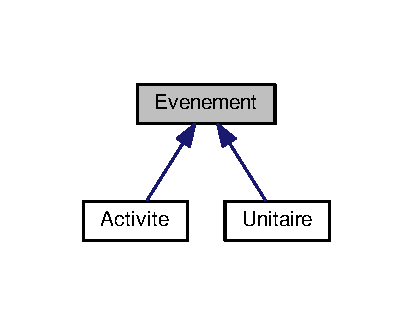
\includegraphics[width=198pt]{class_evenement__inherit__graph}
\end{center}
\end{figure}
\subsection*{Public Member Functions}
\begin{DoxyCompactItemize}
\item 
virtual \hyperlink{class_evenement_a55edc55f582f7992296b10e8a60476c8}{$\sim$\+Evenement} ()
\begin{DoxyCompactList}\small\item\em Destructeur de l\textquotesingle{}événement. \end{DoxyCompactList}\item 
\hyperlink{class_evenement_ab538f1a96d3b5b63f8ce0e89f16bcafd}{Evenement} (\hyperlink{class_t_i_m_e_1_1_duree}{Duree} dur)
\begin{DoxyCompactList}\small\item\em Constructeur de l\textquotesingle{}événement à partir d\textquotesingle{}une durée. \end{DoxyCompactList}\item 
\hyperlink{class_t_i_m_e_1_1_duree}{Duree} \hyperlink{class_evenement_a43c92d1917720282ac6ba3a598fac708}{get\+Duree} () const 
\begin{DoxyCompactList}\small\item\em Renvoie la durée de l\textquotesingle{}événement. \end{DoxyCompactList}\item 
Q\+String \hyperlink{class_evenement_aa5f395f7681426893894fb73eb851459}{get\+Nom} () const 
\begin{DoxyCompactList}\small\item\em Renvoie le nom et l\textquotesingle{}éventuel lieu de l\textquotesingle{}événement en Q\+String. \end{DoxyCompactList}\item 
void \hyperlink{class_evenement_a42e914b00d21eb4377d7c0a242a88e9a}{set\+Duree} (const \hyperlink{class_t_i_m_e_1_1_duree}{Duree} \&dur)
\begin{DoxyCompactList}\small\item\em Modifie la durée de l\textquotesingle{}événement à partir du paramètre \char`\"{}dur\char`\"{}. \end{DoxyCompactList}\item 
virtual void \hyperlink{class_evenement_af217f0cd3d421e3f113a13536ee63593}{afficher} (ostream \&f)=0
\begin{DoxyCompactList}\small\item\em Méthode virtuelle pure d\textquotesingle{}affichage de l\textquotesingle{}événement. \end{DoxyCompactList}\end{DoxyCompactItemize}


\subsection{Detailed Description}
Classe abstraite d\textquotesingle{}éléments pouvant être programmés. 

\subsection{Constructor \& Destructor Documentation}
\hypertarget{class_evenement_a55edc55f582f7992296b10e8a60476c8}{}\index{Evenement@{Evenement}!````~Evenement@{$\sim$\+Evenement}}
\index{````~Evenement@{$\sim$\+Evenement}!Evenement@{Evenement}}
\subsubsection[{$\sim$\+Evenement}]{\setlength{\rightskip}{0pt plus 5cm}virtual Evenement\+::$\sim$\+Evenement (
\begin{DoxyParamCaption}
{}
\end{DoxyParamCaption}
)\hspace{0.3cm}{\ttfamily [inline]}, {\ttfamily [virtual]}}\label{class_evenement_a55edc55f582f7992296b10e8a60476c8}


Destructeur de l\textquotesingle{}événement. 

\hypertarget{class_evenement_ab538f1a96d3b5b63f8ce0e89f16bcafd}{}\index{Evenement@{Evenement}!Evenement@{Evenement}}
\index{Evenement@{Evenement}!Evenement@{Evenement}}
\subsubsection[{Evenement}]{\setlength{\rightskip}{0pt plus 5cm}Evenement\+::\+Evenement (
\begin{DoxyParamCaption}
\item[{{\bf Duree}}]{dur}
\end{DoxyParamCaption}
)\hspace{0.3cm}{\ttfamily [inline]}}\label{class_evenement_ab538f1a96d3b5b63f8ce0e89f16bcafd}


Constructeur de l\textquotesingle{}événement à partir d\textquotesingle{}une durée. 



\subsection{Member Function Documentation}
\hypertarget{class_evenement_af217f0cd3d421e3f113a13536ee63593}{}\index{Evenement@{Evenement}!afficher@{afficher}}
\index{afficher@{afficher}!Evenement@{Evenement}}
\subsubsection[{afficher}]{\setlength{\rightskip}{0pt plus 5cm}virtual void Evenement\+::afficher (
\begin{DoxyParamCaption}
\item[{ostream \&}]{f}
\end{DoxyParamCaption}
)\hspace{0.3cm}{\ttfamily [pure virtual]}}\label{class_evenement_af217f0cd3d421e3f113a13536ee63593}


Méthode virtuelle pure d\textquotesingle{}affichage de l\textquotesingle{}événement. 



Implemented in \hyperlink{class_activite_acf748b87edc5e4a5b78bd5e9364946f3}{Activite}, and \hyperlink{class_unitaire_a98bd645b84e0bd2f378e13774324f7b7}{Unitaire}.

\hypertarget{class_evenement_a43c92d1917720282ac6ba3a598fac708}{}\index{Evenement@{Evenement}!get\+Duree@{get\+Duree}}
\index{get\+Duree@{get\+Duree}!Evenement@{Evenement}}
\subsubsection[{get\+Duree}]{\setlength{\rightskip}{0pt plus 5cm}{\bf Duree} Evenement\+::get\+Duree (
\begin{DoxyParamCaption}
{}
\end{DoxyParamCaption}
) const\hspace{0.3cm}{\ttfamily [inline]}}\label{class_evenement_a43c92d1917720282ac6ba3a598fac708}


Renvoie la durée de l\textquotesingle{}événement. 

\hypertarget{class_evenement_aa5f395f7681426893894fb73eb851459}{}\index{Evenement@{Evenement}!get\+Nom@{get\+Nom}}
\index{get\+Nom@{get\+Nom}!Evenement@{Evenement}}
\subsubsection[{get\+Nom}]{\setlength{\rightskip}{0pt plus 5cm}Q\+String Evenement\+::get\+Nom (
\begin{DoxyParamCaption}
{}
\end{DoxyParamCaption}
) const}\label{class_evenement_aa5f395f7681426893894fb73eb851459}


Renvoie le nom et l\textquotesingle{}éventuel lieu de l\textquotesingle{}événement en Q\+String. 

\hypertarget{class_evenement_a42e914b00d21eb4377d7c0a242a88e9a}{}\index{Evenement@{Evenement}!set\+Duree@{set\+Duree}}
\index{set\+Duree@{set\+Duree}!Evenement@{Evenement}}
\subsubsection[{set\+Duree}]{\setlength{\rightskip}{0pt plus 5cm}void Evenement\+::set\+Duree (
\begin{DoxyParamCaption}
\item[{const {\bf Duree} \&}]{dur}
\end{DoxyParamCaption}
)\hspace{0.3cm}{\ttfamily [inline]}}\label{class_evenement_a42e914b00d21eb4377d7c0a242a88e9a}


Modifie la durée de l\textquotesingle{}événement à partir du paramètre \char`\"{}dur\char`\"{}. 



The documentation for this class was generated from the following files\+:\begin{DoxyCompactItemize}
\item 
L\+O21app/\hyperlink{_calendar_8h}{Calendar.\+h}\item 
L\+O21app/\hyperlink{_calendar_8cpp}{Calendar.\+cpp}\end{DoxyCompactItemize}

\hypertarget{class_event_widget}{}\section{Event\+Widget Class Reference}
\label{class_event_widget}\index{Event\+Widget@{Event\+Widget}}


Classe U\+I affichant un évènement dans l\textquotesingle{}agenda.  




{\ttfamily \#include $<$eventwidget.\+h$>$}



Inheritance diagram for Event\+Widget\+:\nopagebreak
\begin{figure}[H]
\begin{center}
\leavevmode
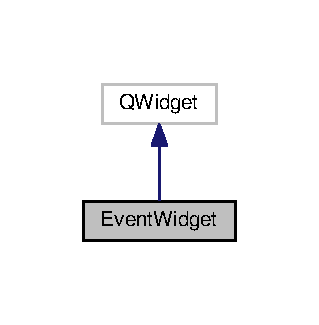
\includegraphics[width=153pt]{class_event_widget__inherit__graph}
\end{center}
\end{figure}


Collaboration diagram for Event\+Widget\+:\nopagebreak
\begin{figure}[H]
\begin{center}
\leavevmode
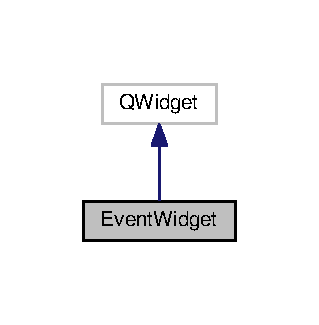
\includegraphics[width=153pt]{class_event_widget__coll__graph}
\end{center}
\end{figure}
\subsection*{Public Member Functions}
\begin{DoxyCompactItemize}
\item 
\hyperlink{class_event_widget_a3db7da18ff8c1b844ecace1a059923c9}{Event\+Widget} (\hyperlink{class_programmation}{Programmation} $\ast$, Q\+Widget $\ast$parent=0)
\item 
\hyperlink{class_event_widget_a88d69e21ca3519d14d22cea87eb81b67}{$\sim$\+Event\+Widget} ()
\end{DoxyCompactItemize}


\subsection{Detailed Description}
Classe U\+I affichant un évènement dans l\textquotesingle{}agenda. 

\subsection{Constructor \& Destructor Documentation}
\hypertarget{class_event_widget_a3db7da18ff8c1b844ecace1a059923c9}{}\index{Event\+Widget@{Event\+Widget}!Event\+Widget@{Event\+Widget}}
\index{Event\+Widget@{Event\+Widget}!Event\+Widget@{Event\+Widget}}
\subsubsection[{Event\+Widget}]{\setlength{\rightskip}{0pt plus 5cm}Event\+Widget\+::\+Event\+Widget (
\begin{DoxyParamCaption}
\item[{{\bf Programmation} $\ast$}]{prog, }
\item[{Q\+Widget $\ast$}]{parent = {\ttfamily 0}}
\end{DoxyParamCaption}
)\hspace{0.3cm}{\ttfamily [explicit]}}\label{class_event_widget_a3db7da18ff8c1b844ecace1a059923c9}
\hypertarget{class_event_widget_a88d69e21ca3519d14d22cea87eb81b67}{}\index{Event\+Widget@{Event\+Widget}!````~Event\+Widget@{$\sim$\+Event\+Widget}}
\index{````~Event\+Widget@{$\sim$\+Event\+Widget}!Event\+Widget@{Event\+Widget}}
\subsubsection[{$\sim$\+Event\+Widget}]{\setlength{\rightskip}{0pt plus 5cm}Event\+Widget\+::$\sim$\+Event\+Widget (
\begin{DoxyParamCaption}
{}
\end{DoxyParamCaption}
)}\label{class_event_widget_a88d69e21ca3519d14d22cea87eb81b67}


The documentation for this class was generated from the following files\+:\begin{DoxyCompactItemize}
\item 
L\+O21app/\hyperlink{eventwidget_8h}{eventwidget.\+h}\item 
L\+O21app/\hyperlink{eventwidget_8cpp}{eventwidget.\+cpp}\end{DoxyCompactItemize}

\hypertarget{class_t_i_m_e_1_1_horaire}{}\section{T\+I\+M\+E\+:\+:Horaire Class Reference}
\label{class_t_i_m_e_1_1_horaire}\index{T\+I\+M\+E\+::\+Horaire@{T\+I\+M\+E\+::\+Horaire}}


Classe permettant de manipuler des horaires L\textquotesingle{}utilisation de cette classe n�cessite des dates valides au sens commun du terme. D�clenchement d\textquotesingle{}exception dans le cas contraire.  




{\ttfamily \#include $<$timing.\+h$>$}

\subsection*{Public Member Functions}
\begin{DoxyCompactItemize}
\item 
\hyperlink{class_t_i_m_e_1_1_horaire_ab833c9dc3a4fdbda3894dbbd72643813}{Horaire} (unsigned short int h, unsigned short int m)
\begin{DoxyCompactList}\small\item\em Constructeur � partir de heure et minute. \end{DoxyCompactList}\item 
\hypertarget{class_t_i_m_e_1_1_horaire_ae4dd22490e383b0662fc5788bd42d370}{}void {\bfseries set\+Horaire} (unsigned short int h, unsigned short int m)\label{class_t_i_m_e_1_1_horaire_ae4dd22490e383b0662fc5788bd42d370}

\item 
\hypertarget{class_t_i_m_e_1_1_horaire_af4f27b26ed338d7fa03659107f813cf8}{}void {\bfseries afficher} (std\+::ostream \&f=std\+::cout) const \label{class_t_i_m_e_1_1_horaire_af4f27b26ed338d7fa03659107f813cf8}

\item 
\hypertarget{class_t_i_m_e_1_1_horaire_ace5d2381e38d80e99c6a84158a4044e3}{}unsigned short int {\bfseries get\+Heure} () const \label{class_t_i_m_e_1_1_horaire_ace5d2381e38d80e99c6a84158a4044e3}

\item 
\hypertarget{class_t_i_m_e_1_1_horaire_a5b0e73a520913fd0588407c1507344a8}{}unsigned short int {\bfseries get\+Minute} () const \label{class_t_i_m_e_1_1_horaire_a5b0e73a520913fd0588407c1507344a8}

\item 
\hypertarget{class_t_i_m_e_1_1_horaire_a30ec21c5b5cad95c1c17c02c66d796a6}{}bool {\bfseries operator$<$} (const \hyperlink{class_t_i_m_e_1_1_horaire}{Horaire} \&h) const \label{class_t_i_m_e_1_1_horaire_a30ec21c5b5cad95c1c17c02c66d796a6}

\end{DoxyCompactItemize}


\subsection{Detailed Description}
Classe permettant de manipuler des horaires L\textquotesingle{}utilisation de cette classe n�cessite des dates valides au sens commun du terme. D�clenchement d\textquotesingle{}exception dans le cas contraire. 

\subsection{Constructor \& Destructor Documentation}
\hypertarget{class_t_i_m_e_1_1_horaire_ab833c9dc3a4fdbda3894dbbd72643813}{}\index{T\+I\+M\+E\+::\+Horaire@{T\+I\+M\+E\+::\+Horaire}!Horaire@{Horaire}}
\index{Horaire@{Horaire}!T\+I\+M\+E\+::\+Horaire@{T\+I\+M\+E\+::\+Horaire}}
\subsubsection[{Horaire}]{\setlength{\rightskip}{0pt plus 5cm}T\+I\+M\+E\+::\+Horaire\+::\+Horaire (
\begin{DoxyParamCaption}
\item[{unsigned short int}]{h, }
\item[{unsigned short int}]{m}
\end{DoxyParamCaption}
)\hspace{0.3cm}{\ttfamily [inline]}}\label{class_t_i_m_e_1_1_horaire_ab833c9dc3a4fdbda3894dbbd72643813}


Constructeur � partir de heure et minute. 


\begin{DoxyParams}{Parameters}
{\em h} & heure avec 0$<$=h$<$=23 \\
\hline
{\em m} & minute avec 0$<$=m$<$=59 \\
\hline
\end{DoxyParams}


The documentation for this class was generated from the following files\+:\begin{DoxyCompactItemize}
\item 
L\+O21app/timing.\+h\item 
L\+O21app/timing.\+cpp\end{DoxyCompactItemize}

\hypertarget{class_t_i_m_e_1_1_intervalle}{}\section{T\+I\+M\+E\+:\+:Intervalle Class Reference}
\label{class_t_i_m_e_1_1_intervalle}\index{T\+I\+M\+E\+::\+Intervalle@{T\+I\+M\+E\+::\+Intervalle}}


Classe permettant de manipuler des intervalles de dates L\textquotesingle{}utilisation de cette classe n�cessite des dates valides au sens commun du terme. D�clenchement d\textquotesingle{}exception dans le cas contraire.  




{\ttfamily \#include $<$timing.\+h$>$}

\subsection*{Public Member Functions}
\begin{DoxyCompactItemize}
\item 
\hyperlink{class_t_i_m_e_1_1_intervalle_a98b63f9c55a777090ec224d61ab26427}{Intervalle} (const \hyperlink{class_t_i_m_e_1_1_date}{Date} \&d, const \hyperlink{class_t_i_m_e_1_1_date}{Date} \&f)
\begin{DoxyCompactList}\small\item\em Constructeur � partir de deux dates. \end{DoxyCompactList}\item 
void \hyperlink{class_t_i_m_e_1_1_intervalle_a729d464967de6618da00b772357dc923}{afficher} (std\+::ostream \&f=std\+::cout) const 
\begin{DoxyCompactList}\small\item\em Affiche l\textquotesingle{}intervalle de dates. \end{DoxyCompactList}\item 
\hyperlink{class_t_i_m_e_1_1_date}{Date} \hyperlink{class_t_i_m_e_1_1_intervalle_a8a9980c16e051af5e08135815cc3d074}{get\+Debut} () const 
\begin{DoxyCompactList}\small\item\em Retourne la date de d�but de l\textquotesingle{}intervalle. \end{DoxyCompactList}\item 
\hyperlink{class_t_i_m_e_1_1_date}{Date} \hyperlink{class_t_i_m_e_1_1_intervalle_a20a035fb9d9720ef94e62e1ef45845c3}{get\+Fin} () const 
\begin{DoxyCompactList}\small\item\em Retourne la date de fin de l\textquotesingle{}intervalle. \end{DoxyCompactList}\item 
int \hyperlink{class_t_i_m_e_1_1_intervalle_adec63857259b690f79de8d16b0ca0c4d}{get\+Duree} () const 
\begin{DoxyCompactList}\small\item\em Retourne le nombre de jours s\textquotesingle{}�coulant entre le d�but et la fin de l\textquotesingle{}intervalle. \end{DoxyCompactList}\item 
bool \hyperlink{class_t_i_m_e_1_1_intervalle_a8f7dca71eb9d8648fa30225360df4fda}{operator\&\&} (const \hyperlink{class_t_i_m_e_1_1_intervalle}{Intervalle} \&v) const 
\begin{DoxyCompactList}\small\item\em I1\&\&I2 Retourne vrai si il y a intersection entre I1 et I2. \end{DoxyCompactList}\item 
\hyperlink{class_t_i_m_e_1_1_intervalle}{Intervalle} \hyperlink{class_t_i_m_e_1_1_intervalle_a9dfead5501b190507a2ffa5c29450ffe}{operator+} (const \hyperlink{class_t_i_m_e_1_1_intervalle}{Intervalle} \&i) const 
\begin{DoxyCompactList}\small\item\em I1+\+I2 Retourne un intervalle union des 2 intervalles I1 et I2 qui se touchent, ie I2.\+debut est le jour du lendemain de I1.\+fin. \end{DoxyCompactList}\end{DoxyCompactItemize}


\subsection{Detailed Description}
Classe permettant de manipuler des intervalles de dates L\textquotesingle{}utilisation de cette classe n�cessite des dates valides au sens commun du terme. D�clenchement d\textquotesingle{}exception dans le cas contraire. 

\subsection{Constructor \& Destructor Documentation}
\hypertarget{class_t_i_m_e_1_1_intervalle_a98b63f9c55a777090ec224d61ab26427}{}\index{T\+I\+M\+E\+::\+Intervalle@{T\+I\+M\+E\+::\+Intervalle}!Intervalle@{Intervalle}}
\index{Intervalle@{Intervalle}!T\+I\+M\+E\+::\+Intervalle@{T\+I\+M\+E\+::\+Intervalle}}
\subsubsection[{Intervalle}]{\setlength{\rightskip}{0pt plus 5cm}Intervalle\+::\+Intervalle (
\begin{DoxyParamCaption}
\item[{const {\bf Date} \&}]{d, }
\item[{const {\bf Date} \&}]{f}
\end{DoxyParamCaption}
)}\label{class_t_i_m_e_1_1_intervalle_a98b63f9c55a777090ec224d61ab26427}


Constructeur � partir de deux dates. 


\begin{DoxyParams}{Parameters}
{\em d} & date de d�but de l\textquotesingle{}intervalle \\
\hline
{\em f} & date de fin de l\textquotesingle{}intervalle. On doit avoir d$<$=f \\
\hline
\end{DoxyParams}


\subsection{Member Function Documentation}
\hypertarget{class_t_i_m_e_1_1_intervalle_a729d464967de6618da00b772357dc923}{}\index{T\+I\+M\+E\+::\+Intervalle@{T\+I\+M\+E\+::\+Intervalle}!afficher@{afficher}}
\index{afficher@{afficher}!T\+I\+M\+E\+::\+Intervalle@{T\+I\+M\+E\+::\+Intervalle}}
\subsubsection[{afficher}]{\setlength{\rightskip}{0pt plus 5cm}void Intervalle\+::afficher (
\begin{DoxyParamCaption}
\item[{std\+::ostream \&}]{f = {\ttfamily std\+:\+:cout}}
\end{DoxyParamCaption}
) const}\label{class_t_i_m_e_1_1_intervalle_a729d464967de6618da00b772357dc923}


Affiche l\textquotesingle{}intervalle de dates. 

\hypertarget{class_t_i_m_e_1_1_intervalle_a8a9980c16e051af5e08135815cc3d074}{}\index{T\+I\+M\+E\+::\+Intervalle@{T\+I\+M\+E\+::\+Intervalle}!get\+Debut@{get\+Debut}}
\index{get\+Debut@{get\+Debut}!T\+I\+M\+E\+::\+Intervalle@{T\+I\+M\+E\+::\+Intervalle}}
\subsubsection[{get\+Debut}]{\setlength{\rightskip}{0pt plus 5cm}{\bf Date} T\+I\+M\+E\+::\+Intervalle\+::get\+Debut (
\begin{DoxyParamCaption}
{}
\end{DoxyParamCaption}
) const\hspace{0.3cm}{\ttfamily [inline]}}\label{class_t_i_m_e_1_1_intervalle_a8a9980c16e051af5e08135815cc3d074}


Retourne la date de d�but de l\textquotesingle{}intervalle. 

\hypertarget{class_t_i_m_e_1_1_intervalle_adec63857259b690f79de8d16b0ca0c4d}{}\index{T\+I\+M\+E\+::\+Intervalle@{T\+I\+M\+E\+::\+Intervalle}!get\+Duree@{get\+Duree}}
\index{get\+Duree@{get\+Duree}!T\+I\+M\+E\+::\+Intervalle@{T\+I\+M\+E\+::\+Intervalle}}
\subsubsection[{get\+Duree}]{\setlength{\rightskip}{0pt plus 5cm}int T\+I\+M\+E\+::\+Intervalle\+::get\+Duree (
\begin{DoxyParamCaption}
{}
\end{DoxyParamCaption}
) const\hspace{0.3cm}{\ttfamily [inline]}}\label{class_t_i_m_e_1_1_intervalle_adec63857259b690f79de8d16b0ca0c4d}


Retourne le nombre de jours s\textquotesingle{}�coulant entre le d�but et la fin de l\textquotesingle{}intervalle. 

\hypertarget{class_t_i_m_e_1_1_intervalle_a20a035fb9d9720ef94e62e1ef45845c3}{}\index{T\+I\+M\+E\+::\+Intervalle@{T\+I\+M\+E\+::\+Intervalle}!get\+Fin@{get\+Fin}}
\index{get\+Fin@{get\+Fin}!T\+I\+M\+E\+::\+Intervalle@{T\+I\+M\+E\+::\+Intervalle}}
\subsubsection[{get\+Fin}]{\setlength{\rightskip}{0pt plus 5cm}{\bf Date} T\+I\+M\+E\+::\+Intervalle\+::get\+Fin (
\begin{DoxyParamCaption}
{}
\end{DoxyParamCaption}
) const\hspace{0.3cm}{\ttfamily [inline]}}\label{class_t_i_m_e_1_1_intervalle_a20a035fb9d9720ef94e62e1ef45845c3}


Retourne la date de fin de l\textquotesingle{}intervalle. 

\hypertarget{class_t_i_m_e_1_1_intervalle_a8f7dca71eb9d8648fa30225360df4fda}{}\index{T\+I\+M\+E\+::\+Intervalle@{T\+I\+M\+E\+::\+Intervalle}!operator\&\&@{operator\&\&}}
\index{operator\&\&@{operator\&\&}!T\+I\+M\+E\+::\+Intervalle@{T\+I\+M\+E\+::\+Intervalle}}
\subsubsection[{operator\&\&}]{\setlength{\rightskip}{0pt plus 5cm}bool Intervalle\+::operator\&\& (
\begin{DoxyParamCaption}
\item[{const {\bf Intervalle} \&}]{v}
\end{DoxyParamCaption}
) const}\label{class_t_i_m_e_1_1_intervalle_a8f7dca71eb9d8648fa30225360df4fda}


I1\&\&I2 Retourne vrai si il y a intersection entre I1 et I2. 

\hypertarget{class_t_i_m_e_1_1_intervalle_a9dfead5501b190507a2ffa5c29450ffe}{}\index{T\+I\+M\+E\+::\+Intervalle@{T\+I\+M\+E\+::\+Intervalle}!operator+@{operator+}}
\index{operator+@{operator+}!T\+I\+M\+E\+::\+Intervalle@{T\+I\+M\+E\+::\+Intervalle}}
\subsubsection[{operator+}]{\setlength{\rightskip}{0pt plus 5cm}{\bf Intervalle} Intervalle\+::operator+ (
\begin{DoxyParamCaption}
\item[{const {\bf Intervalle} \&}]{i}
\end{DoxyParamCaption}
) const}\label{class_t_i_m_e_1_1_intervalle_a9dfead5501b190507a2ffa5c29450ffe}


I1+\+I2 Retourne un intervalle union des 2 intervalles I1 et I2 qui se touchent, ie I2.\+debut est le jour du lendemain de I1.\+fin. 



The documentation for this class was generated from the following files\+:\begin{DoxyCompactItemize}
\item 
L\+O21app/\hyperlink{timing_8h}{timing.\+h}\item 
L\+O21app/\hyperlink{timing_8cpp}{timing.\+cpp}\end{DoxyCompactItemize}

\hypertarget{class_projet_1_1_iterator}{}\section{Projet\+:\+:Iterator Class Reference}
\label{class_projet_1_1_iterator}\index{Projet\+::\+Iterator@{Projet\+::\+Iterator}}


{\ttfamily \#include $<$Calendar.\+h$>$}

\subsection*{Public Member Functions}
\begin{DoxyCompactItemize}
\item 
\hyperlink{class_tache}{Tache} \& \hyperlink{class_projet_1_1_iterator_ad86c65c6828ffdce66bd5d77851acf72}{current} () const 
\item 
bool \hyperlink{class_projet_1_1_iterator_ab1cb3afe4732de443b1a4987a3888675}{is\+Done} () const 
\item 
void \hyperlink{class_projet_1_1_iterator_a2e93894b4d3ec6961fa227f52d720b19}{next} ()
\item 
void \hyperlink{class_projet_1_1_iterator_a2c2d2e1c2a601d6123048efa0d48daf6}{first} ()
\item 
void \hyperlink{class_projet_1_1_iterator_ada239ae15cfc62097e0461034f1be1d7}{suppr} ()
\end{DoxyCompactItemize}
\subsection*{Friends}
\begin{DoxyCompactItemize}
\item 
class \hyperlink{class_projet_1_1_iterator_ab87b41c3faa36955cc370972f5cce344}{Projet}
\end{DoxyCompactItemize}


\subsection{Member Function Documentation}
\hypertarget{class_projet_1_1_iterator_ad86c65c6828ffdce66bd5d77851acf72}{}\index{Projet\+::\+Iterator@{Projet\+::\+Iterator}!current@{current}}
\index{current@{current}!Projet\+::\+Iterator@{Projet\+::\+Iterator}}
\subsubsection[{current}]{\setlength{\rightskip}{0pt plus 5cm}{\bf Tache}\& Projet\+::\+Iterator\+::current (
\begin{DoxyParamCaption}
{}
\end{DoxyParamCaption}
) const\hspace{0.3cm}{\ttfamily [inline]}}\label{class_projet_1_1_iterator_ad86c65c6828ffdce66bd5d77851acf72}
\hypertarget{class_projet_1_1_iterator_a2c2d2e1c2a601d6123048efa0d48daf6}{}\index{Projet\+::\+Iterator@{Projet\+::\+Iterator}!first@{first}}
\index{first@{first}!Projet\+::\+Iterator@{Projet\+::\+Iterator}}
\subsubsection[{first}]{\setlength{\rightskip}{0pt plus 5cm}void Projet\+::\+Iterator\+::first (
\begin{DoxyParamCaption}
{}
\end{DoxyParamCaption}
)\hspace{0.3cm}{\ttfamily [inline]}}\label{class_projet_1_1_iterator_a2c2d2e1c2a601d6123048efa0d48daf6}
\hypertarget{class_projet_1_1_iterator_ab1cb3afe4732de443b1a4987a3888675}{}\index{Projet\+::\+Iterator@{Projet\+::\+Iterator}!is\+Done@{is\+Done}}
\index{is\+Done@{is\+Done}!Projet\+::\+Iterator@{Projet\+::\+Iterator}}
\subsubsection[{is\+Done}]{\setlength{\rightskip}{0pt plus 5cm}bool Projet\+::\+Iterator\+::is\+Done (
\begin{DoxyParamCaption}
{}
\end{DoxyParamCaption}
) const\hspace{0.3cm}{\ttfamily [inline]}}\label{class_projet_1_1_iterator_ab1cb3afe4732de443b1a4987a3888675}
\hypertarget{class_projet_1_1_iterator_a2e93894b4d3ec6961fa227f52d720b19}{}\index{Projet\+::\+Iterator@{Projet\+::\+Iterator}!next@{next}}
\index{next@{next}!Projet\+::\+Iterator@{Projet\+::\+Iterator}}
\subsubsection[{next}]{\setlength{\rightskip}{0pt plus 5cm}void Projet\+::\+Iterator\+::next (
\begin{DoxyParamCaption}
{}
\end{DoxyParamCaption}
)\hspace{0.3cm}{\ttfamily [inline]}}\label{class_projet_1_1_iterator_a2e93894b4d3ec6961fa227f52d720b19}
\hypertarget{class_projet_1_1_iterator_ada239ae15cfc62097e0461034f1be1d7}{}\index{Projet\+::\+Iterator@{Projet\+::\+Iterator}!suppr@{suppr}}
\index{suppr@{suppr}!Projet\+::\+Iterator@{Projet\+::\+Iterator}}
\subsubsection[{suppr}]{\setlength{\rightskip}{0pt plus 5cm}void Projet\+::\+Iterator\+::suppr (
\begin{DoxyParamCaption}
{}
\end{DoxyParamCaption}
)}\label{class_projet_1_1_iterator_ada239ae15cfc62097e0461034f1be1d7}


\subsection{Friends And Related Function Documentation}
\hypertarget{class_projet_1_1_iterator_ab87b41c3faa36955cc370972f5cce344}{}\index{Projet\+::\+Iterator@{Projet\+::\+Iterator}!Projet@{Projet}}
\index{Projet@{Projet}!Projet\+::\+Iterator@{Projet\+::\+Iterator}}
\subsubsection[{Projet}]{\setlength{\rightskip}{0pt plus 5cm}friend class {\bf Projet}\hspace{0.3cm}{\ttfamily [friend]}}\label{class_projet_1_1_iterator_ab87b41c3faa36955cc370972f5cce344}


The documentation for this class was generated from the following files\+:\begin{DoxyCompactItemize}
\item 
L\+O21app/\hyperlink{_calendar_8h}{Calendar.\+h}\item 
L\+O21app/\hyperlink{_calendar_8cpp}{Calendar.\+cpp}\end{DoxyCompactItemize}

\hypertarget{class_tache_1_1_iterator}{}\section{Tache\+:\+:Iterator Class Reference}
\label{class_tache_1_1_iterator}\index{Tache\+::\+Iterator@{Tache\+::\+Iterator}}


{\ttfamily \#include $<$Calendar.\+h$>$}

\subsection*{Public Member Functions}
\begin{DoxyCompactItemize}
\item 
\hyperlink{class_tache}{Tache} \& \hyperlink{class_tache_1_1_iterator_a14d6234f2a8ea2c4e87687375272123a}{current} () const 
\item 
bool \hyperlink{class_tache_1_1_iterator_a8130c3fa6c6cd3c9e2489162e3a01e56}{is\+Done} () const 
\item 
void \hyperlink{class_tache_1_1_iterator_ae9d3e979ec79eb49a73be93391d171a0}{next} ()
\item 
void \hyperlink{class_tache_1_1_iterator_a7329120b9efd311ef5ab48a42c997be8}{first} ()
\end{DoxyCompactItemize}
\subsection*{Friends}
\begin{DoxyCompactItemize}
\item 
class \hyperlink{class_tache_1_1_iterator_affcde2942f74e98f2e6e352cba2a1dc1}{Tache}
\end{DoxyCompactItemize}


\subsection{Member Function Documentation}
\hypertarget{class_tache_1_1_iterator_a14d6234f2a8ea2c4e87687375272123a}{}\index{Tache\+::\+Iterator@{Tache\+::\+Iterator}!current@{current}}
\index{current@{current}!Tache\+::\+Iterator@{Tache\+::\+Iterator}}
\subsubsection[{current}]{\setlength{\rightskip}{0pt plus 5cm}{\bf Tache}\& Tache\+::\+Iterator\+::current (
\begin{DoxyParamCaption}
{}
\end{DoxyParamCaption}
) const\hspace{0.3cm}{\ttfamily [inline]}}\label{class_tache_1_1_iterator_a14d6234f2a8ea2c4e87687375272123a}
\hypertarget{class_tache_1_1_iterator_a7329120b9efd311ef5ab48a42c997be8}{}\index{Tache\+::\+Iterator@{Tache\+::\+Iterator}!first@{first}}
\index{first@{first}!Tache\+::\+Iterator@{Tache\+::\+Iterator}}
\subsubsection[{first}]{\setlength{\rightskip}{0pt plus 5cm}void Tache\+::\+Iterator\+::first (
\begin{DoxyParamCaption}
{}
\end{DoxyParamCaption}
)\hspace{0.3cm}{\ttfamily [inline]}}\label{class_tache_1_1_iterator_a7329120b9efd311ef5ab48a42c997be8}
\hypertarget{class_tache_1_1_iterator_a8130c3fa6c6cd3c9e2489162e3a01e56}{}\index{Tache\+::\+Iterator@{Tache\+::\+Iterator}!is\+Done@{is\+Done}}
\index{is\+Done@{is\+Done}!Tache\+::\+Iterator@{Tache\+::\+Iterator}}
\subsubsection[{is\+Done}]{\setlength{\rightskip}{0pt plus 5cm}bool Tache\+::\+Iterator\+::is\+Done (
\begin{DoxyParamCaption}
{}
\end{DoxyParamCaption}
) const\hspace{0.3cm}{\ttfamily [inline]}}\label{class_tache_1_1_iterator_a8130c3fa6c6cd3c9e2489162e3a01e56}
\hypertarget{class_tache_1_1_iterator_ae9d3e979ec79eb49a73be93391d171a0}{}\index{Tache\+::\+Iterator@{Tache\+::\+Iterator}!next@{next}}
\index{next@{next}!Tache\+::\+Iterator@{Tache\+::\+Iterator}}
\subsubsection[{next}]{\setlength{\rightskip}{0pt plus 5cm}void Tache\+::\+Iterator\+::next (
\begin{DoxyParamCaption}
{}
\end{DoxyParamCaption}
)\hspace{0.3cm}{\ttfamily [inline]}}\label{class_tache_1_1_iterator_ae9d3e979ec79eb49a73be93391d171a0}


\subsection{Friends And Related Function Documentation}
\hypertarget{class_tache_1_1_iterator_affcde2942f74e98f2e6e352cba2a1dc1}{}\index{Tache\+::\+Iterator@{Tache\+::\+Iterator}!Tache@{Tache}}
\index{Tache@{Tache}!Tache\+::\+Iterator@{Tache\+::\+Iterator}}
\subsubsection[{Tache}]{\setlength{\rightskip}{0pt plus 5cm}friend class {\bf Tache}\hspace{0.3cm}{\ttfamily [friend]}}\label{class_tache_1_1_iterator_affcde2942f74e98f2e6e352cba2a1dc1}


The documentation for this class was generated from the following file\+:\begin{DoxyCompactItemize}
\item 
L\+O21app/\hyperlink{_calendar_8h}{Calendar.\+h}\end{DoxyCompactItemize}

\hypertarget{class_projet_manager_1_1_iterator}{}\section{Projet\+Manager\+:\+:Iterator Class Reference}
\label{class_projet_manager_1_1_iterator}\index{Projet\+Manager\+::\+Iterator@{Projet\+Manager\+::\+Iterator}}


{\ttfamily \#include $<$Calendar.\+h$>$}

\subsection*{Public Member Functions}
\begin{DoxyCompactItemize}
\item 
\hyperlink{class_projet}{Projet} \& \hyperlink{class_projet_manager_1_1_iterator_a090d03091123af2199a5afe5c9246675}{current} () const 
\item 
bool \hyperlink{class_projet_manager_1_1_iterator_af1ec6d2831c197dd6239f647ce1f01cd}{is\+Done} () const 
\item 
void \hyperlink{class_projet_manager_1_1_iterator_a6cfc9c4550f68273156cf7ccabc38644}{next} ()
\item 
void \hyperlink{class_projet_manager_1_1_iterator_ae12df7b8aae9acf7ac24a6983957068e}{first} ()
\end{DoxyCompactItemize}
\subsection*{Friends}
\begin{DoxyCompactItemize}
\item 
class \hyperlink{class_projet_manager_1_1_iterator_aaaed9857b3481233fa7c581b5c86151d}{Projet\+Manager}
\end{DoxyCompactItemize}


\subsection{Member Function Documentation}
\hypertarget{class_projet_manager_1_1_iterator_a090d03091123af2199a5afe5c9246675}{}\index{Projet\+Manager\+::\+Iterator@{Projet\+Manager\+::\+Iterator}!current@{current}}
\index{current@{current}!Projet\+Manager\+::\+Iterator@{Projet\+Manager\+::\+Iterator}}
\subsubsection[{current}]{\setlength{\rightskip}{0pt plus 5cm}{\bf Projet}\& Projet\+Manager\+::\+Iterator\+::current (
\begin{DoxyParamCaption}
{}
\end{DoxyParamCaption}
) const\hspace{0.3cm}{\ttfamily [inline]}}\label{class_projet_manager_1_1_iterator_a090d03091123af2199a5afe5c9246675}
\hypertarget{class_projet_manager_1_1_iterator_ae12df7b8aae9acf7ac24a6983957068e}{}\index{Projet\+Manager\+::\+Iterator@{Projet\+Manager\+::\+Iterator}!first@{first}}
\index{first@{first}!Projet\+Manager\+::\+Iterator@{Projet\+Manager\+::\+Iterator}}
\subsubsection[{first}]{\setlength{\rightskip}{0pt plus 5cm}void Projet\+Manager\+::\+Iterator\+::first (
\begin{DoxyParamCaption}
{}
\end{DoxyParamCaption}
)\hspace{0.3cm}{\ttfamily [inline]}}\label{class_projet_manager_1_1_iterator_ae12df7b8aae9acf7ac24a6983957068e}
\hypertarget{class_projet_manager_1_1_iterator_af1ec6d2831c197dd6239f647ce1f01cd}{}\index{Projet\+Manager\+::\+Iterator@{Projet\+Manager\+::\+Iterator}!is\+Done@{is\+Done}}
\index{is\+Done@{is\+Done}!Projet\+Manager\+::\+Iterator@{Projet\+Manager\+::\+Iterator}}
\subsubsection[{is\+Done}]{\setlength{\rightskip}{0pt plus 5cm}bool Projet\+Manager\+::\+Iterator\+::is\+Done (
\begin{DoxyParamCaption}
{}
\end{DoxyParamCaption}
) const\hspace{0.3cm}{\ttfamily [inline]}}\label{class_projet_manager_1_1_iterator_af1ec6d2831c197dd6239f647ce1f01cd}
\hypertarget{class_projet_manager_1_1_iterator_a6cfc9c4550f68273156cf7ccabc38644}{}\index{Projet\+Manager\+::\+Iterator@{Projet\+Manager\+::\+Iterator}!next@{next}}
\index{next@{next}!Projet\+Manager\+::\+Iterator@{Projet\+Manager\+::\+Iterator}}
\subsubsection[{next}]{\setlength{\rightskip}{0pt plus 5cm}void Projet\+Manager\+::\+Iterator\+::next (
\begin{DoxyParamCaption}
{}
\end{DoxyParamCaption}
)\hspace{0.3cm}{\ttfamily [inline]}}\label{class_projet_manager_1_1_iterator_a6cfc9c4550f68273156cf7ccabc38644}


\subsection{Friends And Related Function Documentation}
\hypertarget{class_projet_manager_1_1_iterator_aaaed9857b3481233fa7c581b5c86151d}{}\index{Projet\+Manager\+::\+Iterator@{Projet\+Manager\+::\+Iterator}!Projet\+Manager@{Projet\+Manager}}
\index{Projet\+Manager@{Projet\+Manager}!Projet\+Manager\+::\+Iterator@{Projet\+Manager\+::\+Iterator}}
\subsubsection[{Projet\+Manager}]{\setlength{\rightskip}{0pt plus 5cm}friend class {\bf Projet\+Manager}\hspace{0.3cm}{\ttfamily [friend]}}\label{class_projet_manager_1_1_iterator_aaaed9857b3481233fa7c581b5c86151d}


The documentation for this class was generated from the following file\+:\begin{DoxyCompactItemize}
\item 
L\+O21app/\hyperlink{_calendar_8h}{Calendar.\+h}\end{DoxyCompactItemize}

\hypertarget{class_programmation_manager_1_1_iterator}{}\section{Programmation\+Manager\+:\+:Iterator Class Reference}
\label{class_programmation_manager_1_1_iterator}\index{Programmation\+Manager\+::\+Iterator@{Programmation\+Manager\+::\+Iterator}}


{\ttfamily \#include $<$Calendar.\+h$>$}

\subsection*{Public Member Functions}
\begin{DoxyCompactItemize}
\item 
\hyperlink{class_programmation}{Programmation} \& \hyperlink{class_programmation_manager_1_1_iterator_adc8ca4082b0e46a6d6191e10515f5c48}{current} () const 
\item 
bool \hyperlink{class_programmation_manager_1_1_iterator_ad3b7e90822ee8fcbff8a2067c82ede18}{is\+Done} () const 
\item 
void \hyperlink{class_programmation_manager_1_1_iterator_a281cdb33c35f959bb3c85d920fcba8aa}{next} ()
\item 
void \hyperlink{class_programmation_manager_1_1_iterator_aa0d878e59fc1d28c8d781f088f65214b}{first} ()
\end{DoxyCompactItemize}
\subsection*{Friends}
\begin{DoxyCompactItemize}
\item 
class \hyperlink{class_programmation_manager_1_1_iterator_ade7bfcbf8cec66b12064c8ff25993d73}{Programmation\+Manager}
\end{DoxyCompactItemize}


\subsection{Member Function Documentation}
\hypertarget{class_programmation_manager_1_1_iterator_adc8ca4082b0e46a6d6191e10515f5c48}{}\index{Programmation\+Manager\+::\+Iterator@{Programmation\+Manager\+::\+Iterator}!current@{current}}
\index{current@{current}!Programmation\+Manager\+::\+Iterator@{Programmation\+Manager\+::\+Iterator}}
\subsubsection[{current}]{\setlength{\rightskip}{0pt plus 5cm}{\bf Programmation}\& Programmation\+Manager\+::\+Iterator\+::current (
\begin{DoxyParamCaption}
{}
\end{DoxyParamCaption}
) const\hspace{0.3cm}{\ttfamily [inline]}}\label{class_programmation_manager_1_1_iterator_adc8ca4082b0e46a6d6191e10515f5c48}
\hypertarget{class_programmation_manager_1_1_iterator_aa0d878e59fc1d28c8d781f088f65214b}{}\index{Programmation\+Manager\+::\+Iterator@{Programmation\+Manager\+::\+Iterator}!first@{first}}
\index{first@{first}!Programmation\+Manager\+::\+Iterator@{Programmation\+Manager\+::\+Iterator}}
\subsubsection[{first}]{\setlength{\rightskip}{0pt plus 5cm}void Programmation\+Manager\+::\+Iterator\+::first (
\begin{DoxyParamCaption}
{}
\end{DoxyParamCaption}
)\hspace{0.3cm}{\ttfamily [inline]}}\label{class_programmation_manager_1_1_iterator_aa0d878e59fc1d28c8d781f088f65214b}
\hypertarget{class_programmation_manager_1_1_iterator_ad3b7e90822ee8fcbff8a2067c82ede18}{}\index{Programmation\+Manager\+::\+Iterator@{Programmation\+Manager\+::\+Iterator}!is\+Done@{is\+Done}}
\index{is\+Done@{is\+Done}!Programmation\+Manager\+::\+Iterator@{Programmation\+Manager\+::\+Iterator}}
\subsubsection[{is\+Done}]{\setlength{\rightskip}{0pt plus 5cm}bool Programmation\+Manager\+::\+Iterator\+::is\+Done (
\begin{DoxyParamCaption}
{}
\end{DoxyParamCaption}
) const\hspace{0.3cm}{\ttfamily [inline]}}\label{class_programmation_manager_1_1_iterator_ad3b7e90822ee8fcbff8a2067c82ede18}
\hypertarget{class_programmation_manager_1_1_iterator_a281cdb33c35f959bb3c85d920fcba8aa}{}\index{Programmation\+Manager\+::\+Iterator@{Programmation\+Manager\+::\+Iterator}!next@{next}}
\index{next@{next}!Programmation\+Manager\+::\+Iterator@{Programmation\+Manager\+::\+Iterator}}
\subsubsection[{next}]{\setlength{\rightskip}{0pt plus 5cm}void Programmation\+Manager\+::\+Iterator\+::next (
\begin{DoxyParamCaption}
{}
\end{DoxyParamCaption}
)\hspace{0.3cm}{\ttfamily [inline]}}\label{class_programmation_manager_1_1_iterator_a281cdb33c35f959bb3c85d920fcba8aa}


\subsection{Friends And Related Function Documentation}
\hypertarget{class_programmation_manager_1_1_iterator_ade7bfcbf8cec66b12064c8ff25993d73}{}\index{Programmation\+Manager\+::\+Iterator@{Programmation\+Manager\+::\+Iterator}!Programmation\+Manager@{Programmation\+Manager}}
\index{Programmation\+Manager@{Programmation\+Manager}!Programmation\+Manager\+::\+Iterator@{Programmation\+Manager\+::\+Iterator}}
\subsubsection[{Programmation\+Manager}]{\setlength{\rightskip}{0pt plus 5cm}friend class {\bf Programmation\+Manager}\hspace{0.3cm}{\ttfamily [friend]}}\label{class_programmation_manager_1_1_iterator_ade7bfcbf8cec66b12064c8ff25993d73}


The documentation for this class was generated from the following file\+:\begin{DoxyCompactItemize}
\item 
L\+O21app/\hyperlink{_calendar_8h}{Calendar.\+h}\end{DoxyCompactItemize}

\hypertarget{class_main_window}{}\section{Main\+Window Class Reference}
\label{class_main_window}\index{Main\+Window@{Main\+Window}}


Conserve les pointeurs vers les principaux widgets de la fenêtre. S\textquotesingle{}occupe des actions générales sur ceux-\/ci.  




{\ttfamily \#include $<$Main\+Window.\+h$>$}



Inheritance diagram for Main\+Window\+:\nopagebreak
\begin{figure}[H]
\begin{center}
\leavevmode
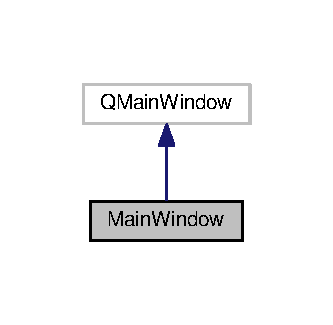
\includegraphics[width=160pt]{class_main_window__inherit__graph}
\end{center}
\end{figure}


Collaboration diagram for Main\+Window\+:\nopagebreak
\begin{figure}[H]
\begin{center}
\leavevmode
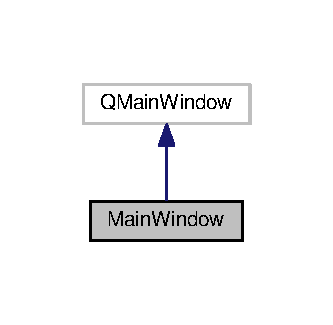
\includegraphics[width=160pt]{class_main_window__coll__graph}
\end{center}
\end{figure}
\subsection*{Public Slots}
\begin{DoxyCompactItemize}
\item 
void \hyperlink{class_main_window_a4e6f43d07f77bfa5ef816fdaeddb2f9c}{tree\+View\+Clicked} (const Q\+Model\+Index \&index)
\begin{DoxyCompactList}\small\item\em On traite le clic sur l\textquotesingle{}item index de la vue Tree\+View. \end{DoxyCompactList}\item 
void \hyperlink{class_main_window_a9221bf94c502faa7f0cb55835dc4f576}{slot\+Ajouter\+Projet} ()
\begin{DoxyCompactList}\small\item\em Ajoute un projet dans le système et sur l\textquotesingle{}arbre. \end{DoxyCompactList}\item 
void \hyperlink{class_main_window_addf6fb45b7869279d5c7b746dfe61429}{slot\+Ajouter\+T\+U} ()
\begin{DoxyCompactList}\small\item\em Ajoute une tache unitaire dans le système et sur l\textquotesingle{}arbre. \end{DoxyCompactList}\item 
void \hyperlink{class_main_window_a4201a4ae86be39f54071eedb95af8291}{slot\+Ajouter\+T\+C} ()
\begin{DoxyCompactList}\small\item\em Ajoute une tache composite dans le système et sur l\textquotesingle{}arbre. \end{DoxyCompactList}\item 
void \hyperlink{class_main_window_a2022b216fafd6461b8b959e791fee853}{slot\+Show\+T\+U} ()
\begin{DoxyCompactList}\small\item\em Lance l\textquotesingle{}affichage de l\textquotesingle{}édition de la tache t. \end{DoxyCompactList}\item 
void \hyperlink{class_main_window_a72cb9533595d3347763e3e485ac01fd6}{slot\+Show\+T\+C} ()
\begin{DoxyCompactList}\small\item\em Lance l\textquotesingle{}affichage de l\textquotesingle{}édition de la tache t. \end{DoxyCompactList}\item 
void \hyperlink{class_main_window_a22bdfd5758d79d8a0dd6b55817f053a0}{slot\+Programmer\+T\+U} ()
\begin{DoxyCompactList}\small\item\em Lance le dialogue pour programmer une tache unitaire. \end{DoxyCompactList}\item 
void \hyperlink{class_main_window_ac54011d65e21b9a451a255c8ab2856d0}{slot\+Programmer\+Activite} ()
\begin{DoxyCompactList}\small\item\em Lance le dialogue pour programmer une activité \end{DoxyCompactList}\end{DoxyCompactItemize}
\subsection*{Public Member Functions}
\begin{DoxyCompactItemize}
\item 
\hyperlink{class_main_window_ae98d00a93bc118200eeef9f9bba1dba7}{$\sim$\+Main\+Window} ()
\item 
\hyperlink{class_main_window_a34c4b4207b46d11a4100c9b19f0e81bb}{Main\+Window} ()
\begin{DoxyCompactList}\small\item\em initialisation de la fenêtre principale \end{DoxyCompactList}\item 
void \hyperlink{class_main_window_a7bbdf27e0ee846803813e53a39a3bf01}{show\+Unitaire} (\hyperlink{class_unitaire}{Unitaire} \&t)
\begin{DoxyCompactList}\small\item\em Affiche l\textquotesingle{}édition d\textquotesingle{}une tache unitaire. \end{DoxyCompactList}\item 
void \hyperlink{class_main_window_a4d74b656f89425afefef0505508befe7}{save\+Unitaire} ()
\begin{DoxyCompactList}\small\item\em Enregistre une tache unitaire. \end{DoxyCompactList}\item 
void \hyperlink{class_main_window_aad741802f157d624081f9588a120f016}{show\+Composite} (\hyperlink{class_composite}{Composite} \&t)
\begin{DoxyCompactList}\small\item\em Affiche l\textquotesingle{}édition d\textquotesingle{} tache composite. \end{DoxyCompactList}\item 
void \hyperlink{class_main_window_a1dfed2a765d3fa7bfb340dd37a5350f1}{show\+Projet} (\hyperlink{class_projet}{Projet} \&p)
\begin{DoxyCompactList}\small\item\em Affiche l\textquotesingle{}édition d\textquotesingle{}un projet. \end{DoxyCompactList}\end{DoxyCompactItemize}


\subsection{Detailed Description}
Conserve les pointeurs vers les principaux widgets de la fenêtre. S\textquotesingle{}occupe des actions générales sur ceux-\/ci. 

Cette classe fait appel aux fonctions d\textquotesingle{}affichage de \hyperlink{_u_i_classes_8h}{U\+I\+Classes.\+h} 

\subsection{Constructor \& Destructor Documentation}
\hypertarget{class_main_window_ae98d00a93bc118200eeef9f9bba1dba7}{}\index{Main\+Window@{Main\+Window}!````~Main\+Window@{$\sim$\+Main\+Window}}
\index{````~Main\+Window@{$\sim$\+Main\+Window}!Main\+Window@{Main\+Window}}
\subsubsection[{$\sim$\+Main\+Window}]{\setlength{\rightskip}{0pt plus 5cm}Main\+Window\+::$\sim$\+Main\+Window (
\begin{DoxyParamCaption}
{}
\end{DoxyParamCaption}
)\hspace{0.3cm}{\ttfamily [inline]}}\label{class_main_window_ae98d00a93bc118200eeef9f9bba1dba7}
\hypertarget{class_main_window_a34c4b4207b46d11a4100c9b19f0e81bb}{}\index{Main\+Window@{Main\+Window}!Main\+Window@{Main\+Window}}
\index{Main\+Window@{Main\+Window}!Main\+Window@{Main\+Window}}
\subsubsection[{Main\+Window}]{\setlength{\rightskip}{0pt plus 5cm}Main\+Window\+::\+Main\+Window (
\begin{DoxyParamCaption}
{}
\end{DoxyParamCaption}
)}\label{class_main_window_a34c4b4207b46d11a4100c9b19f0e81bb}


initialisation de la fenêtre principale 



\subsection{Member Function Documentation}
\hypertarget{class_main_window_a4d74b656f89425afefef0505508befe7}{}\index{Main\+Window@{Main\+Window}!save\+Unitaire@{save\+Unitaire}}
\index{save\+Unitaire@{save\+Unitaire}!Main\+Window@{Main\+Window}}
\subsubsection[{save\+Unitaire}]{\setlength{\rightskip}{0pt plus 5cm}void Main\+Window\+::save\+Unitaire (
\begin{DoxyParamCaption}
{}
\end{DoxyParamCaption}
)}\label{class_main_window_a4d74b656f89425afefef0505508befe7}


Enregistre une tache unitaire. 

\hypertarget{class_main_window_aad741802f157d624081f9588a120f016}{}\index{Main\+Window@{Main\+Window}!show\+Composite@{show\+Composite}}
\index{show\+Composite@{show\+Composite}!Main\+Window@{Main\+Window}}
\subsubsection[{show\+Composite}]{\setlength{\rightskip}{0pt plus 5cm}void Main\+Window\+::show\+Composite (
\begin{DoxyParamCaption}
\item[{{\bf Composite} \&}]{t}
\end{DoxyParamCaption}
)}\label{class_main_window_aad741802f157d624081f9588a120f016}


Affiche l\textquotesingle{}édition d\textquotesingle{} tache composite. 

\hypertarget{class_main_window_a1dfed2a765d3fa7bfb340dd37a5350f1}{}\index{Main\+Window@{Main\+Window}!show\+Projet@{show\+Projet}}
\index{show\+Projet@{show\+Projet}!Main\+Window@{Main\+Window}}
\subsubsection[{show\+Projet}]{\setlength{\rightskip}{0pt plus 5cm}void Main\+Window\+::show\+Projet (
\begin{DoxyParamCaption}
\item[{{\bf Projet} \&}]{p}
\end{DoxyParamCaption}
)}\label{class_main_window_a1dfed2a765d3fa7bfb340dd37a5350f1}


Affiche l\textquotesingle{}édition d\textquotesingle{}un projet. 

\hypertarget{class_main_window_a7bbdf27e0ee846803813e53a39a3bf01}{}\index{Main\+Window@{Main\+Window}!show\+Unitaire@{show\+Unitaire}}
\index{show\+Unitaire@{show\+Unitaire}!Main\+Window@{Main\+Window}}
\subsubsection[{show\+Unitaire}]{\setlength{\rightskip}{0pt plus 5cm}void Main\+Window\+::show\+Unitaire (
\begin{DoxyParamCaption}
\item[{{\bf Unitaire} \&}]{t}
\end{DoxyParamCaption}
)}\label{class_main_window_a7bbdf27e0ee846803813e53a39a3bf01}


Affiche l\textquotesingle{}édition d\textquotesingle{}une tache unitaire. 

\hypertarget{class_main_window_a9221bf94c502faa7f0cb55835dc4f576}{}\index{Main\+Window@{Main\+Window}!slot\+Ajouter\+Projet@{slot\+Ajouter\+Projet}}
\index{slot\+Ajouter\+Projet@{slot\+Ajouter\+Projet}!Main\+Window@{Main\+Window}}
\subsubsection[{slot\+Ajouter\+Projet}]{\setlength{\rightskip}{0pt plus 5cm}void Main\+Window\+::slot\+Ajouter\+Projet (
\begin{DoxyParamCaption}
{}
\end{DoxyParamCaption}
)\hspace{0.3cm}{\ttfamily [slot]}}\label{class_main_window_a9221bf94c502faa7f0cb55835dc4f576}


Ajoute un projet dans le système et sur l\textquotesingle{}arbre. 

\hypertarget{class_main_window_a4201a4ae86be39f54071eedb95af8291}{}\index{Main\+Window@{Main\+Window}!slot\+Ajouter\+T\+C@{slot\+Ajouter\+T\+C}}
\index{slot\+Ajouter\+T\+C@{slot\+Ajouter\+T\+C}!Main\+Window@{Main\+Window}}
\subsubsection[{slot\+Ajouter\+T\+C}]{\setlength{\rightskip}{0pt plus 5cm}void Main\+Window\+::slot\+Ajouter\+T\+C (
\begin{DoxyParamCaption}
{}
\end{DoxyParamCaption}
)\hspace{0.3cm}{\ttfamily [slot]}}\label{class_main_window_a4201a4ae86be39f54071eedb95af8291}


Ajoute une tache composite dans le système et sur l\textquotesingle{}arbre. 

\hypertarget{class_main_window_addf6fb45b7869279d5c7b746dfe61429}{}\index{Main\+Window@{Main\+Window}!slot\+Ajouter\+T\+U@{slot\+Ajouter\+T\+U}}
\index{slot\+Ajouter\+T\+U@{slot\+Ajouter\+T\+U}!Main\+Window@{Main\+Window}}
\subsubsection[{slot\+Ajouter\+T\+U}]{\setlength{\rightskip}{0pt plus 5cm}void Main\+Window\+::slot\+Ajouter\+T\+U (
\begin{DoxyParamCaption}
{}
\end{DoxyParamCaption}
)\hspace{0.3cm}{\ttfamily [slot]}}\label{class_main_window_addf6fb45b7869279d5c7b746dfe61429}


Ajoute une tache unitaire dans le système et sur l\textquotesingle{}arbre. 

\hypertarget{class_main_window_ac54011d65e21b9a451a255c8ab2856d0}{}\index{Main\+Window@{Main\+Window}!slot\+Programmer\+Activite@{slot\+Programmer\+Activite}}
\index{slot\+Programmer\+Activite@{slot\+Programmer\+Activite}!Main\+Window@{Main\+Window}}
\subsubsection[{slot\+Programmer\+Activite}]{\setlength{\rightskip}{0pt plus 5cm}void Main\+Window\+::slot\+Programmer\+Activite (
\begin{DoxyParamCaption}
{}
\end{DoxyParamCaption}
)\hspace{0.3cm}{\ttfamily [slot]}}\label{class_main_window_ac54011d65e21b9a451a255c8ab2856d0}


Lance le dialogue pour programmer une activité 

\hypertarget{class_main_window_a22bdfd5758d79d8a0dd6b55817f053a0}{}\index{Main\+Window@{Main\+Window}!slot\+Programmer\+T\+U@{slot\+Programmer\+T\+U}}
\index{slot\+Programmer\+T\+U@{slot\+Programmer\+T\+U}!Main\+Window@{Main\+Window}}
\subsubsection[{slot\+Programmer\+T\+U}]{\setlength{\rightskip}{0pt plus 5cm}void Main\+Window\+::slot\+Programmer\+T\+U (
\begin{DoxyParamCaption}
{}
\end{DoxyParamCaption}
)\hspace{0.3cm}{\ttfamily [slot]}}\label{class_main_window_a22bdfd5758d79d8a0dd6b55817f053a0}


Lance le dialogue pour programmer une tache unitaire. 

\hypertarget{class_main_window_a72cb9533595d3347763e3e485ac01fd6}{}\index{Main\+Window@{Main\+Window}!slot\+Show\+T\+C@{slot\+Show\+T\+C}}
\index{slot\+Show\+T\+C@{slot\+Show\+T\+C}!Main\+Window@{Main\+Window}}
\subsubsection[{slot\+Show\+T\+C}]{\setlength{\rightskip}{0pt plus 5cm}void Main\+Window\+::slot\+Show\+T\+C (
\begin{DoxyParamCaption}
{}
\end{DoxyParamCaption}
)\hspace{0.3cm}{\ttfamily [slot]}}\label{class_main_window_a72cb9533595d3347763e3e485ac01fd6}


Lance l\textquotesingle{}affichage de l\textquotesingle{}édition de la tache t. 

\hypertarget{class_main_window_a2022b216fafd6461b8b959e791fee853}{}\index{Main\+Window@{Main\+Window}!slot\+Show\+T\+U@{slot\+Show\+T\+U}}
\index{slot\+Show\+T\+U@{slot\+Show\+T\+U}!Main\+Window@{Main\+Window}}
\subsubsection[{slot\+Show\+T\+U}]{\setlength{\rightskip}{0pt plus 5cm}void Main\+Window\+::slot\+Show\+T\+U (
\begin{DoxyParamCaption}
{}
\end{DoxyParamCaption}
)\hspace{0.3cm}{\ttfamily [slot]}}\label{class_main_window_a2022b216fafd6461b8b959e791fee853}


Lance l\textquotesingle{}affichage de l\textquotesingle{}édition de la tache t. 

\hypertarget{class_main_window_a4e6f43d07f77bfa5ef816fdaeddb2f9c}{}\index{Main\+Window@{Main\+Window}!tree\+View\+Clicked@{tree\+View\+Clicked}}
\index{tree\+View\+Clicked@{tree\+View\+Clicked}!Main\+Window@{Main\+Window}}
\subsubsection[{tree\+View\+Clicked}]{\setlength{\rightskip}{0pt plus 5cm}void Main\+Window\+::tree\+View\+Clicked (
\begin{DoxyParamCaption}
\item[{const Q\+Model\+Index \&}]{index}
\end{DoxyParamCaption}
)\hspace{0.3cm}{\ttfamily [slot]}}\label{class_main_window_a4e6f43d07f77bfa5ef816fdaeddb2f9c}


On traite le clic sur l\textquotesingle{}item index de la vue Tree\+View. 



The documentation for this class was generated from the following files\+:\begin{DoxyCompactItemize}
\item 
L\+O21app/\hyperlink{_main_window_8h}{Main\+Window.\+h}\item 
L\+O21app/\hyperlink{_main_window_8cpp}{Main\+Window.\+cpp}\end{DoxyCompactItemize}

\hypertarget{class_t_i_m_e_1_1_periode}{}\section{T\+I\+M\+E\+:\+:Periode Class Reference}
\label{class_t_i_m_e_1_1_periode}\index{T\+I\+M\+E\+::\+Periode@{T\+I\+M\+E\+::\+Periode}}


Classe permettant de manipuler des periodes exprim�es en jours/mois/ann�es L\textquotesingle{}utilisation de cette classe n�cessite des dates valides au sens commun du terme. D�clenchement d\textquotesingle{}exception dans le cas contraire.  




{\ttfamily \#include $<$timing.\+h$>$}

\subsection*{Public Member Functions}
\begin{DoxyCompactItemize}
\item 
\hyperlink{class_t_i_m_e_1_1_periode_ab5de9657ef88d74ca2cdc4a49b963ba6}{Periode} (unsigned int j, unsigned int m, unsigned int a)
\begin{DoxyCompactList}\small\item\em Constructeur � partir de jour/mois/ann�e. \end{DoxyCompactList}\item 
void \hyperlink{class_t_i_m_e_1_1_periode_a0e97a115f8a2e6b503fdcb82ee1d8f08}{afficher} (std\+::ostream \&f=std\+::cout) const 
\end{DoxyCompactItemize}


\subsection{Detailed Description}
Classe permettant de manipuler des periodes exprim�es en jours/mois/ann�es L\textquotesingle{}utilisation de cette classe n�cessite des dates valides au sens commun du terme. D�clenchement d\textquotesingle{}exception dans le cas contraire. 

\subsection{Constructor \& Destructor Documentation}
\hypertarget{class_t_i_m_e_1_1_periode_ab5de9657ef88d74ca2cdc4a49b963ba6}{}\index{T\+I\+M\+E\+::\+Periode@{T\+I\+M\+E\+::\+Periode}!Periode@{Periode}}
\index{Periode@{Periode}!T\+I\+M\+E\+::\+Periode@{T\+I\+M\+E\+::\+Periode}}
\subsubsection[{Periode}]{\setlength{\rightskip}{0pt plus 5cm}Periode\+::\+Periode (
\begin{DoxyParamCaption}
\item[{unsigned int}]{j, }
\item[{unsigned int}]{m, }
\item[{unsigned int}]{a}
\end{DoxyParamCaption}
)}\label{class_t_i_m_e_1_1_periode_ab5de9657ef88d74ca2cdc4a49b963ba6}


Constructeur � partir de jour/mois/ann�e. 


\begin{DoxyParams}{Parameters}
{\em j} & nombre de jours avec 0$<$=j$<$=364 \\
\hline
{\em m} & nombre de mois avec 0$<$=m$<$=11 \\
\hline
{\em a} & nombre d\textquotesingle{}ann�es \\
\hline
\end{DoxyParams}


\subsection{Member Function Documentation}
\hypertarget{class_t_i_m_e_1_1_periode_a0e97a115f8a2e6b503fdcb82ee1d8f08}{}\index{T\+I\+M\+E\+::\+Periode@{T\+I\+M\+E\+::\+Periode}!afficher@{afficher}}
\index{afficher@{afficher}!T\+I\+M\+E\+::\+Periode@{T\+I\+M\+E\+::\+Periode}}
\subsubsection[{afficher}]{\setlength{\rightskip}{0pt plus 5cm}void T\+I\+M\+E\+::\+Periode\+::afficher (
\begin{DoxyParamCaption}
\item[{std\+::ostream \&}]{f = {\ttfamily std\+:\+:cout}}
\end{DoxyParamCaption}
) const\hspace{0.3cm}{\ttfamily [inline]}}\label{class_t_i_m_e_1_1_periode_a0e97a115f8a2e6b503fdcb82ee1d8f08}


The documentation for this class was generated from the following files\+:\begin{DoxyCompactItemize}
\item 
L\+O21app/\hyperlink{timing_8h}{timing.\+h}\item 
L\+O21app/\hyperlink{timing_8cpp}{timing.\+cpp}\end{DoxyCompactItemize}

\hypertarget{class_programmation}{}\section{Programmation Class Reference}
\label{class_programmation}\index{Programmation@{Programmation}}
\subsection*{Public Member Functions}
\begin{DoxyCompactItemize}
\item 
\hypertarget{class_programmation_a2c557f9f87c56133c658e2b14cd68ab9}{}{\bfseries Programmation} (const \hyperlink{class_unitaire}{Unitaire} \&t, const \hyperlink{class_t_i_m_e_1_1_date}{Date} \&d, const \hyperlink{class_t_i_m_e_1_1_horaire}{Horaire} \&h)\label{class_programmation_a2c557f9f87c56133c658e2b14cd68ab9}

\item 
\hypertarget{class_programmation_a7395fca93b007fbd741e6a331b531ab9}{}const \hyperlink{class_tache}{Tache} \& \hyperlink{class_programmation_a7395fca93b007fbd741e6a331b531ab9}{get\+Tache} () const \label{class_programmation_a7395fca93b007fbd741e6a331b531ab9}

\begin{DoxyCompactList}\small\item\em accesseur \end{DoxyCompactList}\item 
\hypertarget{class_programmation_abab51a44ecfa15becd790571d80074e8}{}\hyperlink{class_t_i_m_e_1_1_date}{Date} \hyperlink{class_programmation_abab51a44ecfa15becd790571d80074e8}{get\+Date} () const \label{class_programmation_abab51a44ecfa15becd790571d80074e8}

\begin{DoxyCompactList}\small\item\em accesseur \end{DoxyCompactList}\item 
\hypertarget{class_programmation_af4b33fc2e67826566fff3ba43f637c4f}{}\hyperlink{class_t_i_m_e_1_1_horaire}{Horaire} \hyperlink{class_programmation_af4b33fc2e67826566fff3ba43f637c4f}{get\+Horaire} () const \label{class_programmation_af4b33fc2e67826566fff3ba43f637c4f}

\begin{DoxyCompactList}\small\item\em accesseur \end{DoxyCompactList}\end{DoxyCompactItemize}


The documentation for this class was generated from the following file\+:\begin{DoxyCompactItemize}
\item 
L\+O21app/Calendar.\+h\end{DoxyCompactItemize}

\hypertarget{class_programmation_activite}{}\section{Programmation\+Activite Class Reference}
\label{class_programmation_activite}\index{Programmation\+Activite@{Programmation\+Activite}}


Dialogue de programmation d\textquotesingle{}une activité  




{\ttfamily \#include $<$U\+I\+Classes.\+h$>$}



Inheritance diagram for Programmation\+Activite\+:\nopagebreak
\begin{figure}[H]
\begin{center}
\leavevmode
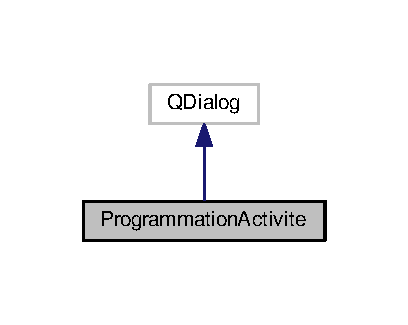
\includegraphics[width=196pt]{class_programmation_activite__inherit__graph}
\end{center}
\end{figure}


Collaboration diagram for Programmation\+Activite\+:\nopagebreak
\begin{figure}[H]
\begin{center}
\leavevmode
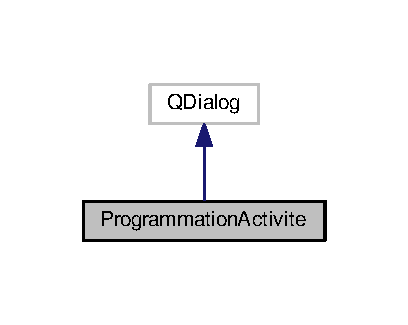
\includegraphics[width=196pt]{class_programmation_activite__coll__graph}
\end{center}
\end{figure}
\subsection*{Public Slots}
\begin{DoxyCompactItemize}
\item 
virtual void \hyperlink{class_programmation_activite_a411643dc5f9fc094a834b38e85472503}{slot\+Save} ()
\end{DoxyCompactItemize}
\subsection*{Signals}
\begin{DoxyCompactItemize}
\item 
void \hyperlink{class_programmation_activite_a7101e83ceba3f4eb7302bafa4862011f}{activite\+Programmee} ()
\begin{DoxyCompactList}\small\item\em Une activité a été programmée. \end{DoxyCompactList}\end{DoxyCompactItemize}
\subsection*{Public Member Functions}
\begin{DoxyCompactItemize}
\item 
\hyperlink{class_programmation_activite_ae36ea268d121dddc0633ed9bfc7fc3b6}{Programmation\+Activite} ()
\end{DoxyCompactItemize}
\subsection*{Public Attributes}
\begin{DoxyCompactItemize}
\item 
Q\+Line\+Edit $\ast$ \hyperlink{class_programmation_activite_a4abe5a47855bf2955f81f75c48d1e705}{titre}
\item 
Q\+Line\+Edit $\ast$ \hyperlink{class_programmation_activite_ad11789d8e5720d094c2b18f0ab79c8fd}{lieu}
\item 
Q\+Spin\+Box $\ast$ \hyperlink{class_programmation_activite_a7edeef86cb3b134a39b3289c11930cfe}{h\+Horaire}
\item 
Q\+Spin\+Box $\ast$ \hyperlink{class_programmation_activite_a4f962ff214fd6decf90e97cde1c1b7d5}{m\+Horaire}
\item 
Q\+Spin\+Box $\ast$ \hyperlink{class_programmation_activite_af5e275e33582e76962bc991b042951a7}{h\+Duree}
\item 
Q\+Spin\+Box $\ast$ \hyperlink{class_programmation_activite_af7138f1541605f97e14984c977ad5632}{m\+Duree}
\item 
Q\+Calendar\+Widget $\ast$ \hyperlink{class_programmation_activite_a4530b3c068395d0a0d87d2f7d00d6ff0}{date}
\item 
Q\+Form\+Layout $\ast$ \hyperlink{class_programmation_activite_a1cf55e2cad5a97ba1ba0238bfe804eb9}{form\+Layout}
\end{DoxyCompactItemize}


\subsection{Detailed Description}
Dialogue de programmation d\textquotesingle{}une activité 

Demande à l\textquotesingle{}utilisateur de saisir les caractéristiques d\textquotesingle{}une activité et la programme. 

\subsection{Constructor \& Destructor Documentation}
\hypertarget{class_programmation_activite_ae36ea268d121dddc0633ed9bfc7fc3b6}{}\index{Programmation\+Activite@{Programmation\+Activite}!Programmation\+Activite@{Programmation\+Activite}}
\index{Programmation\+Activite@{Programmation\+Activite}!Programmation\+Activite@{Programmation\+Activite}}
\subsubsection[{Programmation\+Activite}]{\setlength{\rightskip}{0pt plus 5cm}Programmation\+Activite\+::\+Programmation\+Activite (
\begin{DoxyParamCaption}
{}
\end{DoxyParamCaption}
)}\label{class_programmation_activite_ae36ea268d121dddc0633ed9bfc7fc3b6}


\subsection{Member Function Documentation}
\hypertarget{class_programmation_activite_a7101e83ceba3f4eb7302bafa4862011f}{}\index{Programmation\+Activite@{Programmation\+Activite}!activite\+Programmee@{activite\+Programmee}}
\index{activite\+Programmee@{activite\+Programmee}!Programmation\+Activite@{Programmation\+Activite}}
\subsubsection[{activite\+Programmee}]{\setlength{\rightskip}{0pt plus 5cm}void Programmation\+Activite\+::activite\+Programmee (
\begin{DoxyParamCaption}
{}
\end{DoxyParamCaption}
)\hspace{0.3cm}{\ttfamily [signal]}}\label{class_programmation_activite_a7101e83ceba3f4eb7302bafa4862011f}


Une activité a été programmée. 

\hypertarget{class_programmation_activite_a411643dc5f9fc094a834b38e85472503}{}\index{Programmation\+Activite@{Programmation\+Activite}!slot\+Save@{slot\+Save}}
\index{slot\+Save@{slot\+Save}!Programmation\+Activite@{Programmation\+Activite}}
\subsubsection[{slot\+Save}]{\setlength{\rightskip}{0pt plus 5cm}void Programmation\+Activite\+::slot\+Save (
\begin{DoxyParamCaption}
{}
\end{DoxyParamCaption}
)\hspace{0.3cm}{\ttfamily [virtual]}, {\ttfamily [slot]}}\label{class_programmation_activite_a411643dc5f9fc094a834b38e85472503}


\subsection{Member Data Documentation}
\hypertarget{class_programmation_activite_a4530b3c068395d0a0d87d2f7d00d6ff0}{}\index{Programmation\+Activite@{Programmation\+Activite}!date@{date}}
\index{date@{date}!Programmation\+Activite@{Programmation\+Activite}}
\subsubsection[{date}]{\setlength{\rightskip}{0pt plus 5cm}Q\+Calendar\+Widget$\ast$ Programmation\+Activite\+::date}\label{class_programmation_activite_a4530b3c068395d0a0d87d2f7d00d6ff0}
\hypertarget{class_programmation_activite_a1cf55e2cad5a97ba1ba0238bfe804eb9}{}\index{Programmation\+Activite@{Programmation\+Activite}!form\+Layout@{form\+Layout}}
\index{form\+Layout@{form\+Layout}!Programmation\+Activite@{Programmation\+Activite}}
\subsubsection[{form\+Layout}]{\setlength{\rightskip}{0pt plus 5cm}Q\+Form\+Layout$\ast$ Programmation\+Activite\+::form\+Layout}\label{class_programmation_activite_a1cf55e2cad5a97ba1ba0238bfe804eb9}
\hypertarget{class_programmation_activite_af5e275e33582e76962bc991b042951a7}{}\index{Programmation\+Activite@{Programmation\+Activite}!h\+Duree@{h\+Duree}}
\index{h\+Duree@{h\+Duree}!Programmation\+Activite@{Programmation\+Activite}}
\subsubsection[{h\+Duree}]{\setlength{\rightskip}{0pt plus 5cm}Q\+Spin\+Box$\ast$ Programmation\+Activite\+::h\+Duree}\label{class_programmation_activite_af5e275e33582e76962bc991b042951a7}
\hypertarget{class_programmation_activite_a7edeef86cb3b134a39b3289c11930cfe}{}\index{Programmation\+Activite@{Programmation\+Activite}!h\+Horaire@{h\+Horaire}}
\index{h\+Horaire@{h\+Horaire}!Programmation\+Activite@{Programmation\+Activite}}
\subsubsection[{h\+Horaire}]{\setlength{\rightskip}{0pt plus 5cm}Q\+Spin\+Box$\ast$ Programmation\+Activite\+::h\+Horaire}\label{class_programmation_activite_a7edeef86cb3b134a39b3289c11930cfe}
\hypertarget{class_programmation_activite_ad11789d8e5720d094c2b18f0ab79c8fd}{}\index{Programmation\+Activite@{Programmation\+Activite}!lieu@{lieu}}
\index{lieu@{lieu}!Programmation\+Activite@{Programmation\+Activite}}
\subsubsection[{lieu}]{\setlength{\rightskip}{0pt plus 5cm}Q\+Line\+Edit$\ast$ Programmation\+Activite\+::lieu}\label{class_programmation_activite_ad11789d8e5720d094c2b18f0ab79c8fd}
\hypertarget{class_programmation_activite_af7138f1541605f97e14984c977ad5632}{}\index{Programmation\+Activite@{Programmation\+Activite}!m\+Duree@{m\+Duree}}
\index{m\+Duree@{m\+Duree}!Programmation\+Activite@{Programmation\+Activite}}
\subsubsection[{m\+Duree}]{\setlength{\rightskip}{0pt plus 5cm}Q\+Spin\+Box$\ast$ Programmation\+Activite\+::m\+Duree}\label{class_programmation_activite_af7138f1541605f97e14984c977ad5632}
\hypertarget{class_programmation_activite_a4f962ff214fd6decf90e97cde1c1b7d5}{}\index{Programmation\+Activite@{Programmation\+Activite}!m\+Horaire@{m\+Horaire}}
\index{m\+Horaire@{m\+Horaire}!Programmation\+Activite@{Programmation\+Activite}}
\subsubsection[{m\+Horaire}]{\setlength{\rightskip}{0pt plus 5cm}Q\+Spin\+Box$\ast$ Programmation\+Activite\+::m\+Horaire}\label{class_programmation_activite_a4f962ff214fd6decf90e97cde1c1b7d5}
\hypertarget{class_programmation_activite_a4abe5a47855bf2955f81f75c48d1e705}{}\index{Programmation\+Activite@{Programmation\+Activite}!titre@{titre}}
\index{titre@{titre}!Programmation\+Activite@{Programmation\+Activite}}
\subsubsection[{titre}]{\setlength{\rightskip}{0pt plus 5cm}Q\+Line\+Edit$\ast$ Programmation\+Activite\+::titre}\label{class_programmation_activite_a4abe5a47855bf2955f81f75c48d1e705}


The documentation for this class was generated from the following files\+:\begin{DoxyCompactItemize}
\item 
L\+O21app/\hyperlink{_u_i_classes_8h}{U\+I\+Classes.\+h}\item 
L\+O21app/\hyperlink{_u_i_classes_8cpp}{U\+I\+Classes.\+cpp}\end{DoxyCompactItemize}

\hypertarget{class_programmation_manager}{}\section{Programmation\+Manager Class Reference}
\label{class_programmation_manager}\index{Programmation\+Manager@{Programmation\+Manager}}


Classe composite de \hyperlink{class_programmation}{Programmation} La classe applique le designe pattern singleton et possède un iterateur sur le tableau de pointeurs de Programmations.  




{\ttfamily \#include $<$Calendar.\+h$>$}



Inheritance diagram for Programmation\+Manager\+:\nopagebreak
\begin{figure}[H]
\begin{center}
\leavevmode
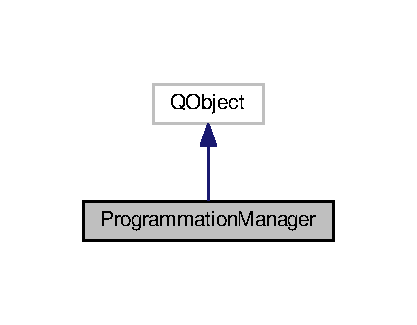
\includegraphics[width=200pt]{class_programmation_manager__inherit__graph}
\end{center}
\end{figure}


Collaboration diagram for Programmation\+Manager\+:\nopagebreak
\begin{figure}[H]
\begin{center}
\leavevmode
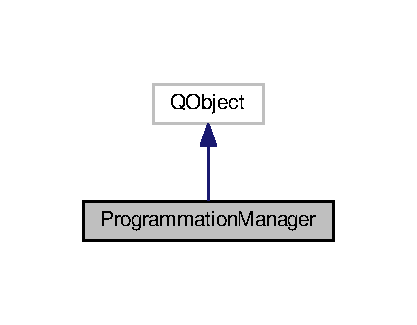
\includegraphics[width=200pt]{class_programmation_manager__coll__graph}
\end{center}
\end{figure}
\subsection*{Classes}
\begin{DoxyCompactItemize}
\item 
class \hyperlink{class_programmation_manager_1_1_iterator}{Iterator}
\end{DoxyCompactItemize}
\subsection*{Signals}
\begin{DoxyCompactItemize}
\item 
void \hyperlink{class_programmation_manager_ad6f6dbec484d80425f498460650a0649}{programmations\+Changed} ()
\begin{DoxyCompactList}\small\item\em Signal de changement de programmation. \end{DoxyCompactList}\end{DoxyCompactItemize}
\subsection*{Public Member Functions}
\begin{DoxyCompactItemize}
\item 
\hyperlink{class_programmation}{Programmation} $\ast$ \hyperlink{class_programmation_manager_a43fd958e37bf4a78b845006aa5551bec}{trouver\+Programmation} (\hyperlink{class_evenement}{Evenement} \&e) const 
\begin{DoxyCompactList}\small\item\em Renvoie le pointeur de la programmation de l\textquotesingle{}événement correspondant si elle existe dans le tableau. \end{DoxyCompactList}\item 
\hyperlink{class_programmation}{Programmation} $\ast$ \hyperlink{class_programmation_manager_ab52ba49ca1d79add9f6d83f8f9386b7e}{trouver\+Programmation} (const \hyperlink{class_evenement}{Evenement} \&e) const 
\begin{DoxyCompactList}\small\item\em Renvoie le pointeur de la programmation de l\textquotesingle{}événement const correspondant si elle existe dans le tableau. \end{DoxyCompactList}\item 
void \hyperlink{class_programmation_manager_a8b6067aba53b0389d30c485c9a544769}{ajouter\+Programmation} (\hyperlink{class_unitaire}{Unitaire} \&e, const \hyperlink{class_t_i_m_e_1_1_date}{Date} \&d, const \hyperlink{class_t_i_m_e_1_1_horaire}{Horaire} \&h, \hyperlink{class_t_i_m_e_1_1_duree}{Duree} dur)
\begin{DoxyCompactList}\small\item\em Crée une programmation d\textquotesingle{}une \hyperlink{class_tache}{Tache} \hyperlink{class_unitaire}{Unitaire} et stocke le pointeur dans le tableau programmations. \end{DoxyCompactList}\item 
void \hyperlink{class_programmation_manager_a3451eabd67b35163c6213eed9b2f3733}{ajouter\+Programmation} (\hyperlink{class_activite}{Activite} \&e, const \hyperlink{class_t_i_m_e_1_1_date}{Date} \&d, const \hyperlink{class_t_i_m_e_1_1_horaire}{Horaire} \&h, const \hyperlink{class_t_i_m_e_1_1_duree}{Duree} \&dur)
\begin{DoxyCompactList}\small\item\em Crée une programmation d\textquotesingle{}une Activité et stocke le pointeur dans le tableau programmations. \end{DoxyCompactList}\item 
\hyperlink{class_programmation_manager_1_1_iterator}{Iterator} \hyperlink{class_programmation_manager_aaff6e0852f9e7ec4aeb47f6ef976fdf9}{get\+Iterator} ()
\begin{DoxyCompactList}\small\item\em Renvoie un iterateur sur programmations. \end{DoxyCompactList}\end{DoxyCompactItemize}
\subsection*{Static Public Member Functions}
\begin{DoxyCompactItemize}
\item 
static \hyperlink{class_programmation_manager}{Programmation\+Manager} \& \hyperlink{class_programmation_manager_a9da2fc647972756d1f8cdf91d4017c25}{get\+Instance} ()
\begin{DoxyCompactList}\small\item\em Renvoie la seule instance de \hyperlink{class_programmation_manager}{Programmation\+Manager}. \end{DoxyCompactList}\item 
static void \hyperlink{class_programmation_manager_a94e3fcb28ea7c632dc6750c33949d712}{liberer\+Instance} ()
\begin{DoxyCompactList}\small\item\em Libère l\textquotesingle{}unique instance de \hyperlink{class_programmation_manager}{Programmation\+Manager}. \end{DoxyCompactList}\end{DoxyCompactItemize}


\subsection{Detailed Description}
Classe composite de \hyperlink{class_programmation}{Programmation} La classe applique le designe pattern singleton et possède un iterateur sur le tableau de pointeurs de Programmations. 

\subsection{Member Function Documentation}
\hypertarget{class_programmation_manager_a8b6067aba53b0389d30c485c9a544769}{}\index{Programmation\+Manager@{Programmation\+Manager}!ajouter\+Programmation@{ajouter\+Programmation}}
\index{ajouter\+Programmation@{ajouter\+Programmation}!Programmation\+Manager@{Programmation\+Manager}}
\subsubsection[{ajouter\+Programmation}]{\setlength{\rightskip}{0pt plus 5cm}void Programmation\+Manager\+::ajouter\+Programmation (
\begin{DoxyParamCaption}
\item[{{\bf Unitaire} \&}]{e, }
\item[{const {\bf Date} \&}]{d, }
\item[{const {\bf Horaire} \&}]{h, }
\item[{{\bf Duree}}]{dur}
\end{DoxyParamCaption}
)}\label{class_programmation_manager_a8b6067aba53b0389d30c485c9a544769}


Crée une programmation d\textquotesingle{}une \hyperlink{class_tache}{Tache} \hyperlink{class_unitaire}{Unitaire} et stocke le pointeur dans le tableau programmations. 

\hypertarget{class_programmation_manager_a3451eabd67b35163c6213eed9b2f3733}{}\index{Programmation\+Manager@{Programmation\+Manager}!ajouter\+Programmation@{ajouter\+Programmation}}
\index{ajouter\+Programmation@{ajouter\+Programmation}!Programmation\+Manager@{Programmation\+Manager}}
\subsubsection[{ajouter\+Programmation}]{\setlength{\rightskip}{0pt plus 5cm}void Programmation\+Manager\+::ajouter\+Programmation (
\begin{DoxyParamCaption}
\item[{{\bf Activite} \&}]{e, }
\item[{const {\bf Date} \&}]{d, }
\item[{const {\bf Horaire} \&}]{h, }
\item[{const {\bf Duree} \&}]{dur}
\end{DoxyParamCaption}
)}\label{class_programmation_manager_a3451eabd67b35163c6213eed9b2f3733}


Crée une programmation d\textquotesingle{}une Activité et stocke le pointeur dans le tableau programmations. 

\hypertarget{class_programmation_manager_a9da2fc647972756d1f8cdf91d4017c25}{}\index{Programmation\+Manager@{Programmation\+Manager}!get\+Instance@{get\+Instance}}
\index{get\+Instance@{get\+Instance}!Programmation\+Manager@{Programmation\+Manager}}
\subsubsection[{get\+Instance}]{\setlength{\rightskip}{0pt plus 5cm}{\bf Programmation\+Manager} \& Programmation\+Manager\+::get\+Instance (
\begin{DoxyParamCaption}
{}
\end{DoxyParamCaption}
)\hspace{0.3cm}{\ttfamily [static]}}\label{class_programmation_manager_a9da2fc647972756d1f8cdf91d4017c25}


Renvoie la seule instance de \hyperlink{class_programmation_manager}{Programmation\+Manager}. 

\hypertarget{class_programmation_manager_aaff6e0852f9e7ec4aeb47f6ef976fdf9}{}\index{Programmation\+Manager@{Programmation\+Manager}!get\+Iterator@{get\+Iterator}}
\index{get\+Iterator@{get\+Iterator}!Programmation\+Manager@{Programmation\+Manager}}
\subsubsection[{get\+Iterator}]{\setlength{\rightskip}{0pt plus 5cm}{\bf Iterator} Programmation\+Manager\+::get\+Iterator (
\begin{DoxyParamCaption}
{}
\end{DoxyParamCaption}
)\hspace{0.3cm}{\ttfamily [inline]}}\label{class_programmation_manager_aaff6e0852f9e7ec4aeb47f6ef976fdf9}


Renvoie un iterateur sur programmations. 

\hypertarget{class_programmation_manager_a94e3fcb28ea7c632dc6750c33949d712}{}\index{Programmation\+Manager@{Programmation\+Manager}!liberer\+Instance@{liberer\+Instance}}
\index{liberer\+Instance@{liberer\+Instance}!Programmation\+Manager@{Programmation\+Manager}}
\subsubsection[{liberer\+Instance}]{\setlength{\rightskip}{0pt plus 5cm}void Programmation\+Manager\+::liberer\+Instance (
\begin{DoxyParamCaption}
{}
\end{DoxyParamCaption}
)\hspace{0.3cm}{\ttfamily [static]}}\label{class_programmation_manager_a94e3fcb28ea7c632dc6750c33949d712}


Libère l\textquotesingle{}unique instance de \hyperlink{class_programmation_manager}{Programmation\+Manager}. 

\hypertarget{class_programmation_manager_ad6f6dbec484d80425f498460650a0649}{}\index{Programmation\+Manager@{Programmation\+Manager}!programmations\+Changed@{programmations\+Changed}}
\index{programmations\+Changed@{programmations\+Changed}!Programmation\+Manager@{Programmation\+Manager}}
\subsubsection[{programmations\+Changed}]{\setlength{\rightskip}{0pt plus 5cm}void Programmation\+Manager\+::programmations\+Changed (
\begin{DoxyParamCaption}
{}
\end{DoxyParamCaption}
)\hspace{0.3cm}{\ttfamily [signal]}}\label{class_programmation_manager_ad6f6dbec484d80425f498460650a0649}


Signal de changement de programmation. 

\hypertarget{class_programmation_manager_a43fd958e37bf4a78b845006aa5551bec}{}\index{Programmation\+Manager@{Programmation\+Manager}!trouver\+Programmation@{trouver\+Programmation}}
\index{trouver\+Programmation@{trouver\+Programmation}!Programmation\+Manager@{Programmation\+Manager}}
\subsubsection[{trouver\+Programmation}]{\setlength{\rightskip}{0pt plus 5cm}{\bf Programmation} $\ast$ Programmation\+Manager\+::trouver\+Programmation (
\begin{DoxyParamCaption}
\item[{{\bf Evenement} \&}]{e}
\end{DoxyParamCaption}
) const}\label{class_programmation_manager_a43fd958e37bf4a78b845006aa5551bec}


Renvoie le pointeur de la programmation de l\textquotesingle{}événement correspondant si elle existe dans le tableau. 

\hypertarget{class_programmation_manager_ab52ba49ca1d79add9f6d83f8f9386b7e}{}\index{Programmation\+Manager@{Programmation\+Manager}!trouver\+Programmation@{trouver\+Programmation}}
\index{trouver\+Programmation@{trouver\+Programmation}!Programmation\+Manager@{Programmation\+Manager}}
\subsubsection[{trouver\+Programmation}]{\setlength{\rightskip}{0pt plus 5cm}{\bf Programmation} $\ast$ Programmation\+Manager\+::trouver\+Programmation (
\begin{DoxyParamCaption}
\item[{const {\bf Evenement} \&}]{e}
\end{DoxyParamCaption}
) const}\label{class_programmation_manager_ab52ba49ca1d79add9f6d83f8f9386b7e}


Renvoie le pointeur de la programmation de l\textquotesingle{}événement const correspondant si elle existe dans le tableau. 



The documentation for this class was generated from the following files\+:\begin{DoxyCompactItemize}
\item 
L\+O21app/\hyperlink{_calendar_8h}{Calendar.\+h}\item 
L\+O21app/\hyperlink{_calendar_8cpp}{Calendar.\+cpp}\end{DoxyCompactItemize}

\hypertarget{class_programmation_tache}{}\section{Programmation\+Tache Class Reference}
\label{class_programmation_tache}\index{Programmation\+Tache@{Programmation\+Tache}}


Programme la tache sélectionnée dans le tree view.  




{\ttfamily \#include $<$U\+I\+Classes.\+h$>$}



Inheritance diagram for Programmation\+Tache\+:\nopagebreak
\begin{figure}[H]
\begin{center}
\leavevmode
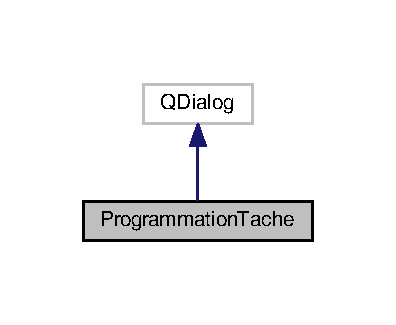
\includegraphics[width=190pt]{class_programmation_tache__inherit__graph}
\end{center}
\end{figure}


Collaboration diagram for Programmation\+Tache\+:\nopagebreak
\begin{figure}[H]
\begin{center}
\leavevmode
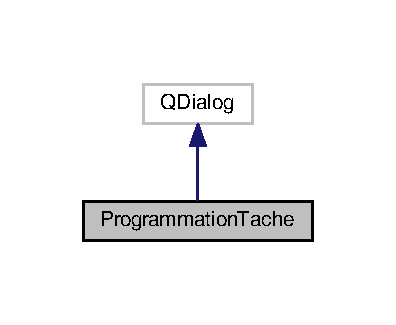
\includegraphics[width=190pt]{class_programmation_tache__coll__graph}
\end{center}
\end{figure}
\subsection*{Public Slots}
\begin{DoxyCompactItemize}
\item 
virtual void \hyperlink{class_programmation_tache_a00d0c96edf68ce7418d368121a901fdc}{slot\+Save} ()
\end{DoxyCompactItemize}
\subsection*{Signals}
\begin{DoxyCompactItemize}
\item 
void \hyperlink{class_programmation_tache_a86deb26ff4326577af72514a09c6eb35}{tache\+Programmee} ()
\begin{DoxyCompactList}\small\item\em Une tache a été programmée. \end{DoxyCompactList}\end{DoxyCompactItemize}
\subsection*{Public Member Functions}
\begin{DoxyCompactItemize}
\item 
\hyperlink{class_programmation_tache_afea7e682b7e6065d906e7d1479d5ed3d}{Programmation\+Tache} (\hyperlink{class_unitaire}{Unitaire} $\ast$t)
\end{DoxyCompactItemize}
\subsection*{Public Attributes}
\begin{DoxyCompactItemize}
\item 
Q\+Label $\ast$ \hyperlink{class_programmation_tache_a6eea8febad907f0705eb3a9e8cc3fbde}{titre}
\item 
Q\+Spin\+Box $\ast$ \hyperlink{class_programmation_tache_a19daaa27a4939dd499b80f57ed84a1fe}{h\+Horaire}
\item 
Q\+Spin\+Box $\ast$ \hyperlink{class_programmation_tache_a2d966e73c014f058565681c5e75e4894}{m\+Horaire}
\item 
Q\+Spin\+Box $\ast$ \hyperlink{class_programmation_tache_afe61c430a658d980efa98c7438e69138}{h\+Duree}
\item 
Q\+Spin\+Box $\ast$ \hyperlink{class_programmation_tache_a0761dfd09ef37d029a8d38f2db32d69d}{m\+Duree}
\item 
Q\+Calendar\+Widget $\ast$ \hyperlink{class_programmation_tache_a65d7216f9e6aa7b663f67cdc38b6b2c2}{date}
\item 
Q\+Form\+Layout $\ast$ \hyperlink{class_programmation_tache_a9de086b288d85e80903c18a8200a1cae}{form\+Layout}
\end{DoxyCompactItemize}


\subsection{Detailed Description}
Programme la tache sélectionnée dans le tree view. 

Vérifie qu\textquotesingle{}une programmation est possible et demande à l\textquotesingle{}utilisateur de la saisir 

\subsection{Constructor \& Destructor Documentation}
\hypertarget{class_programmation_tache_afea7e682b7e6065d906e7d1479d5ed3d}{}\index{Programmation\+Tache@{Programmation\+Tache}!Programmation\+Tache@{Programmation\+Tache}}
\index{Programmation\+Tache@{Programmation\+Tache}!Programmation\+Tache@{Programmation\+Tache}}
\subsubsection[{Programmation\+Tache}]{\setlength{\rightskip}{0pt plus 5cm}Programmation\+Tache\+::\+Programmation\+Tache (
\begin{DoxyParamCaption}
\item[{{\bf Unitaire} $\ast$}]{t}
\end{DoxyParamCaption}
)}\label{class_programmation_tache_afea7e682b7e6065d906e7d1479d5ed3d}


\subsection{Member Function Documentation}
\hypertarget{class_programmation_tache_a00d0c96edf68ce7418d368121a901fdc}{}\index{Programmation\+Tache@{Programmation\+Tache}!slot\+Save@{slot\+Save}}
\index{slot\+Save@{slot\+Save}!Programmation\+Tache@{Programmation\+Tache}}
\subsubsection[{slot\+Save}]{\setlength{\rightskip}{0pt plus 5cm}void Programmation\+Tache\+::slot\+Save (
\begin{DoxyParamCaption}
{}
\end{DoxyParamCaption}
)\hspace{0.3cm}{\ttfamily [virtual]}, {\ttfamily [slot]}}\label{class_programmation_tache_a00d0c96edf68ce7418d368121a901fdc}
\hypertarget{class_programmation_tache_a86deb26ff4326577af72514a09c6eb35}{}\index{Programmation\+Tache@{Programmation\+Tache}!tache\+Programmee@{tache\+Programmee}}
\index{tache\+Programmee@{tache\+Programmee}!Programmation\+Tache@{Programmation\+Tache}}
\subsubsection[{tache\+Programmee}]{\setlength{\rightskip}{0pt plus 5cm}void Programmation\+Tache\+::tache\+Programmee (
\begin{DoxyParamCaption}
{}
\end{DoxyParamCaption}
)\hspace{0.3cm}{\ttfamily [signal]}}\label{class_programmation_tache_a86deb26ff4326577af72514a09c6eb35}


Une tache a été programmée. 



\subsection{Member Data Documentation}
\hypertarget{class_programmation_tache_a65d7216f9e6aa7b663f67cdc38b6b2c2}{}\index{Programmation\+Tache@{Programmation\+Tache}!date@{date}}
\index{date@{date}!Programmation\+Tache@{Programmation\+Tache}}
\subsubsection[{date}]{\setlength{\rightskip}{0pt plus 5cm}Q\+Calendar\+Widget$\ast$ Programmation\+Tache\+::date}\label{class_programmation_tache_a65d7216f9e6aa7b663f67cdc38b6b2c2}
\hypertarget{class_programmation_tache_a9de086b288d85e80903c18a8200a1cae}{}\index{Programmation\+Tache@{Programmation\+Tache}!form\+Layout@{form\+Layout}}
\index{form\+Layout@{form\+Layout}!Programmation\+Tache@{Programmation\+Tache}}
\subsubsection[{form\+Layout}]{\setlength{\rightskip}{0pt plus 5cm}Q\+Form\+Layout$\ast$ Programmation\+Tache\+::form\+Layout}\label{class_programmation_tache_a9de086b288d85e80903c18a8200a1cae}
\hypertarget{class_programmation_tache_afe61c430a658d980efa98c7438e69138}{}\index{Programmation\+Tache@{Programmation\+Tache}!h\+Duree@{h\+Duree}}
\index{h\+Duree@{h\+Duree}!Programmation\+Tache@{Programmation\+Tache}}
\subsubsection[{h\+Duree}]{\setlength{\rightskip}{0pt plus 5cm}Q\+Spin\+Box$\ast$ Programmation\+Tache\+::h\+Duree}\label{class_programmation_tache_afe61c430a658d980efa98c7438e69138}
\hypertarget{class_programmation_tache_a19daaa27a4939dd499b80f57ed84a1fe}{}\index{Programmation\+Tache@{Programmation\+Tache}!h\+Horaire@{h\+Horaire}}
\index{h\+Horaire@{h\+Horaire}!Programmation\+Tache@{Programmation\+Tache}}
\subsubsection[{h\+Horaire}]{\setlength{\rightskip}{0pt plus 5cm}Q\+Spin\+Box$\ast$ Programmation\+Tache\+::h\+Horaire}\label{class_programmation_tache_a19daaa27a4939dd499b80f57ed84a1fe}
\hypertarget{class_programmation_tache_a0761dfd09ef37d029a8d38f2db32d69d}{}\index{Programmation\+Tache@{Programmation\+Tache}!m\+Duree@{m\+Duree}}
\index{m\+Duree@{m\+Duree}!Programmation\+Tache@{Programmation\+Tache}}
\subsubsection[{m\+Duree}]{\setlength{\rightskip}{0pt plus 5cm}Q\+Spin\+Box$\ast$ Programmation\+Tache\+::m\+Duree}\label{class_programmation_tache_a0761dfd09ef37d029a8d38f2db32d69d}
\hypertarget{class_programmation_tache_a2d966e73c014f058565681c5e75e4894}{}\index{Programmation\+Tache@{Programmation\+Tache}!m\+Horaire@{m\+Horaire}}
\index{m\+Horaire@{m\+Horaire}!Programmation\+Tache@{Programmation\+Tache}}
\subsubsection[{m\+Horaire}]{\setlength{\rightskip}{0pt plus 5cm}Q\+Spin\+Box$\ast$ Programmation\+Tache\+::m\+Horaire}\label{class_programmation_tache_a2d966e73c014f058565681c5e75e4894}
\hypertarget{class_programmation_tache_a6eea8febad907f0705eb3a9e8cc3fbde}{}\index{Programmation\+Tache@{Programmation\+Tache}!titre@{titre}}
\index{titre@{titre}!Programmation\+Tache@{Programmation\+Tache}}
\subsubsection[{titre}]{\setlength{\rightskip}{0pt plus 5cm}Q\+Label$\ast$ Programmation\+Tache\+::titre}\label{class_programmation_tache_a6eea8febad907f0705eb3a9e8cc3fbde}


The documentation for this class was generated from the following files\+:\begin{DoxyCompactItemize}
\item 
L\+O21app/\hyperlink{_u_i_classes_8h}{U\+I\+Classes.\+h}\item 
L\+O21app/\hyperlink{_u_i_classes_8cpp}{U\+I\+Classes.\+cpp}\end{DoxyCompactItemize}

\hypertarget{class_projet}{}\section{Projet Class Reference}
\label{class_projet}\index{Projet@{Projet}}


Un ensemble de tache à réaliser.  




{\ttfamily \#include $<$Calendar.\+h$>$}

\subsection*{Classes}
\begin{DoxyCompactItemize}
\item 
class \hyperlink{class_projet_1_1_iterator}{Iterator}
\end{DoxyCompactItemize}
\subsection*{Public Member Functions}
\begin{DoxyCompactItemize}
\item 
\hypertarget{class_projet_abc4ef9586bab910e754d4f88943df720}{}string \hyperlink{class_projet_abc4ef9586bab910e754d4f88943df720}{get\+Nom} () const \label{class_projet_abc4ef9586bab910e754d4f88943df720}

\begin{DoxyCompactList}\small\item\em accesseur \end{DoxyCompactList}\item 
\hypertarget{class_projet_acb3ac5233074e53f0263bd50b4e0bdec}{}\hyperlink{class_projet_1_1_iterator}{Iterator} {\bfseries get\+Iterator} ()\label{class_projet_acb3ac5233074e53f0263bd50b4e0bdec}

\end{DoxyCompactItemize}
\subsection*{Friends}
\begin{DoxyCompactItemize}
\item 
\hypertarget{class_projet_a9830fc407400559db7e7783cc10a9394}{}class {\bfseries Iterator}\label{class_projet_a9830fc407400559db7e7783cc10a9394}

\end{DoxyCompactItemize}


\subsection{Detailed Description}
Un ensemble de tache à réaliser. 

The documentation for this class was generated from the following file\+:\begin{DoxyCompactItemize}
\item 
L\+O21app/Calendar.\+h\end{DoxyCompactItemize}

\hypertarget{class_projet_manager}{}\section{Projet\+Manager Class Reference}
\label{class_projet_manager}\index{Projet\+Manager@{Projet\+Manager}}


Classe composite des Projets La classe applique le designe pattern singleton et possède un iterateur sur le tableau de pointeurs de Projets.  




{\ttfamily \#include $<$Calendar.\+h$>$}

\subsection*{Classes}
\begin{DoxyCompactItemize}
\item 
class \hyperlink{class_projet_manager_1_1_iterator}{Iterator}
\end{DoxyCompactItemize}
\subsection*{Public Member Functions}
\begin{DoxyCompactItemize}
\item 
\hyperlink{class_projet}{Projet} \& \hyperlink{class_projet_manager_a1deef0505a26f2b14e7d2a35e1fead59}{ajouter\+Projet} (const string \&nom, const string \&file, const \hyperlink{class_t_i_m_e_1_1_date}{Date} \&dispo)
\begin{DoxyCompactList}\small\item\em Crée un \hyperlink{class_projet}{Projet} et garde son pointeur dans le tableau projets, à partir d\textquotesingle{}n nom, d\textquotesingle{}un nom de fichier et d\textquotesingle{}une date de disponibilité \end{DoxyCompactList}\item 
\hyperlink{class_projet}{Projet} \& \hyperlink{class_projet_manager_aef6c8f10713e04d8e5e2592a8ab611e9}{get\+Projet} (const string \&id)
\begin{DoxyCompactList}\small\item\em Renvoie une référence vers le projet correspondant à id s\textquotesingle{}il existe dans le tableau projets. \end{DoxyCompactList}\item 
const \hyperlink{class_projet}{Projet} \& \hyperlink{class_projet_manager_a6287b1b73903f5458895135b2e6ca8f8}{get\+Projet} (const string \&code) const 
\begin{DoxyCompactList}\small\item\em Renvoie une référence const vers le projet correspondant à id s\textquotesingle{}il existe dans le tableau projets. \end{DoxyCompactList}\item 
\hyperlink{class_projet_manager_1_1_iterator}{Iterator} \hyperlink{class_projet_manager_ad326876aa4985f2b05a19d0750a8aa5e}{get\+Iterator} ()
\begin{DoxyCompactList}\small\item\em Renvoie un itérateur sur le tableau projets. \end{DoxyCompactList}\end{DoxyCompactItemize}
\subsection*{Static Public Member Functions}
\begin{DoxyCompactItemize}
\item 
static \hyperlink{class_projet_manager}{Projet\+Manager} \& \hyperlink{class_projet_manager_af0b8d536c3d208289033d6a3b757fac9}{get\+Instance} ()
\begin{DoxyCompactList}\small\item\em Renvoie la seule instance de \hyperlink{class_projet_manager}{Projet\+Manager}. \end{DoxyCompactList}\item 
static void \hyperlink{class_projet_manager_ab1b9396cdda866051d03ac5eae7f7e9d}{liberer\+Instance} ()
\begin{DoxyCompactList}\small\item\em Libère l\textquotesingle{}instance de \hyperlink{class_projet_manager}{Projet\+Manager}. \end{DoxyCompactList}\end{DoxyCompactItemize}


\subsection{Detailed Description}
Classe composite des Projets La classe applique le designe pattern singleton et possède un iterateur sur le tableau de pointeurs de Projets. 

\subsection{Member Function Documentation}
\hypertarget{class_projet_manager_a1deef0505a26f2b14e7d2a35e1fead59}{}\index{Projet\+Manager@{Projet\+Manager}!ajouter\+Projet@{ajouter\+Projet}}
\index{ajouter\+Projet@{ajouter\+Projet}!Projet\+Manager@{Projet\+Manager}}
\subsubsection[{ajouter\+Projet}]{\setlength{\rightskip}{0pt plus 5cm}{\bf Projet} \& Projet\+Manager\+::ajouter\+Projet (
\begin{DoxyParamCaption}
\item[{const string \&}]{nom, }
\item[{const string \&}]{file, }
\item[{const {\bf Date} \&}]{dispo}
\end{DoxyParamCaption}
)}\label{class_projet_manager_a1deef0505a26f2b14e7d2a35e1fead59}


Crée un \hyperlink{class_projet}{Projet} et garde son pointeur dans le tableau projets, à partir d\textquotesingle{}n nom, d\textquotesingle{}un nom de fichier et d\textquotesingle{}une date de disponibilité 

\hypertarget{class_projet_manager_af0b8d536c3d208289033d6a3b757fac9}{}\index{Projet\+Manager@{Projet\+Manager}!get\+Instance@{get\+Instance}}
\index{get\+Instance@{get\+Instance}!Projet\+Manager@{Projet\+Manager}}
\subsubsection[{get\+Instance}]{\setlength{\rightskip}{0pt plus 5cm}{\bf Projet\+Manager} \& Projet\+Manager\+::get\+Instance (
\begin{DoxyParamCaption}
{}
\end{DoxyParamCaption}
)\hspace{0.3cm}{\ttfamily [static]}}\label{class_projet_manager_af0b8d536c3d208289033d6a3b757fac9}


Renvoie la seule instance de \hyperlink{class_projet_manager}{Projet\+Manager}. 

\hypertarget{class_projet_manager_ad326876aa4985f2b05a19d0750a8aa5e}{}\index{Projet\+Manager@{Projet\+Manager}!get\+Iterator@{get\+Iterator}}
\index{get\+Iterator@{get\+Iterator}!Projet\+Manager@{Projet\+Manager}}
\subsubsection[{get\+Iterator}]{\setlength{\rightskip}{0pt plus 5cm}{\bf Iterator} Projet\+Manager\+::get\+Iterator (
\begin{DoxyParamCaption}
{}
\end{DoxyParamCaption}
)\hspace{0.3cm}{\ttfamily [inline]}}\label{class_projet_manager_ad326876aa4985f2b05a19d0750a8aa5e}


Renvoie un itérateur sur le tableau projets. 

\hypertarget{class_projet_manager_aef6c8f10713e04d8e5e2592a8ab611e9}{}\index{Projet\+Manager@{Projet\+Manager}!get\+Projet@{get\+Projet}}
\index{get\+Projet@{get\+Projet}!Projet\+Manager@{Projet\+Manager}}
\subsubsection[{get\+Projet}]{\setlength{\rightskip}{0pt plus 5cm}{\bf Projet} \& Projet\+Manager\+::get\+Projet (
\begin{DoxyParamCaption}
\item[{const string \&}]{id}
\end{DoxyParamCaption}
)}\label{class_projet_manager_aef6c8f10713e04d8e5e2592a8ab611e9}


Renvoie une référence vers le projet correspondant à id s\textquotesingle{}il existe dans le tableau projets. 

\hypertarget{class_projet_manager_a6287b1b73903f5458895135b2e6ca8f8}{}\index{Projet\+Manager@{Projet\+Manager}!get\+Projet@{get\+Projet}}
\index{get\+Projet@{get\+Projet}!Projet\+Manager@{Projet\+Manager}}
\subsubsection[{get\+Projet}]{\setlength{\rightskip}{0pt plus 5cm}const {\bf Projet}\& Projet\+Manager\+::get\+Projet (
\begin{DoxyParamCaption}
\item[{const string \&}]{code}
\end{DoxyParamCaption}
) const}\label{class_projet_manager_a6287b1b73903f5458895135b2e6ca8f8}


Renvoie une référence const vers le projet correspondant à id s\textquotesingle{}il existe dans le tableau projets. 

\hypertarget{class_projet_manager_ab1b9396cdda866051d03ac5eae7f7e9d}{}\index{Projet\+Manager@{Projet\+Manager}!liberer\+Instance@{liberer\+Instance}}
\index{liberer\+Instance@{liberer\+Instance}!Projet\+Manager@{Projet\+Manager}}
\subsubsection[{liberer\+Instance}]{\setlength{\rightskip}{0pt plus 5cm}void Projet\+Manager\+::liberer\+Instance (
\begin{DoxyParamCaption}
{}
\end{DoxyParamCaption}
)\hspace{0.3cm}{\ttfamily [static]}}\label{class_projet_manager_ab1b9396cdda866051d03ac5eae7f7e9d}


Libère l\textquotesingle{}instance de \hyperlink{class_projet_manager}{Projet\+Manager}. 



The documentation for this class was generated from the following files\+:\begin{DoxyCompactItemize}
\item 
L\+O21app/\hyperlink{_calendar_8h}{Calendar.\+h}\item 
L\+O21app/\hyperlink{_calendar_8cpp}{Calendar.\+cpp}\end{DoxyCompactItemize}

\hypertarget{class_tache}{}\section{Tache Class Reference}
\label{class_tache}\index{Tache@{Tache}}


Classe abstraite de taches composant \hyperlink{class_projet}{Projet}.  




{\ttfamily \#include $<$Calendar.\+h$>$}



Inheritance diagram for Tache\+:\nopagebreak
\begin{figure}[H]
\begin{center}
\leavevmode
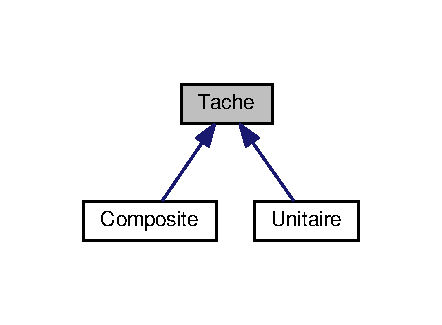
\includegraphics[width=212pt]{class_tache__inherit__graph}
\end{center}
\end{figure}
\subsection*{Classes}
\begin{DoxyCompactItemize}
\item 
class \hyperlink{class_tache_1_1_iterator}{Iterator}
\end{DoxyCompactItemize}
\subsection*{Public Member Functions}
\begin{DoxyCompactItemize}
\item 
unsigned int \hyperlink{class_tache_ac597ce580ad0b32c373b329d4da839ad}{get\+Nb\+Pred} ()
\begin{DoxyCompactList}\small\item\em Renvoie le nombre d\textquotesingle{}éléments de prec. \end{DoxyCompactList}\item 
\hyperlink{class_projet}{Projet} $\ast$ \hyperlink{class_tache_aa6d1abc3712b5a8b571bb3c131129ac7}{get\+Projet} () const 
\begin{DoxyCompactList}\small\item\em Renvoie un pointeur vers le projet parent de la tache. \end{DoxyCompactList}\item 
virtual \hyperlink{class_tache_acefc2a88516ef4d8bd7b25afcf769e9c}{$\sim$\+Tache} ()
\begin{DoxyCompactList}\small\item\em Desctructeur de la tache. \end{DoxyCompactList}\item 
\hyperlink{class_tache_a026b068c4e49643d6fec30c9b915ddca}{Tache} (const string \&id, const string \&t, const \hyperlink{class_t_i_m_e_1_1_date}{Date} \&dispo, const \hyperlink{class_t_i_m_e_1_1_date}{Date} \&deadline, \hyperlink{class_projet}{Projet} $\ast$p)
\item 
virtual void \hyperlink{class_tache_a6a13b4138a46f22e632bf9d35f155c09}{add\+Item} (\hyperlink{class_tache}{Tache} $\ast$t)
\begin{DoxyCompactList}\small\item\em Ajoute le pointeur de tache dans prec comme nouvelle contrainte de précédence. \end{DoxyCompactList}\item 
\hyperlink{class_tache}{Tache} \& \hyperlink{class_tache_ab29bfb6c79337fbc9dc5618195f12f8d}{get\+Precedence} (const string \&id)
\begin{DoxyCompactList}\small\item\em Renvoie une référence vers la tache désignée par id si elle existe dans prec. \end{DoxyCompactList}\item 
const \hyperlink{class_tache}{Tache} \& \hyperlink{class_tache_af995526e12eed76ffa2a4ba7b6fb7a90}{get\+Precedence} (const string \&code) const 
\begin{DoxyCompactList}\small\item\em Renvoie une const référence vers la tache désignée par id si elle existe dans prec. \end{DoxyCompactList}\item 
bool \hyperlink{class_tache_a72df18190512de6ca437492a3664d05a}{is\+Precedence} () const 
\begin{DoxyCompactList}\small\item\em Indique par booléen si la tache a des précédences ou non. \end{DoxyCompactList}\item 
virtual bool \hyperlink{class_tache_ae873dc0bfe552ea39c34f430d56f3846}{is\+Precedence\+Potentielle} (const string \&id)
\begin{DoxyCompactList}\small\item\em Indique si la tache désignée par id est une précédence potentielle ou non pour la tache. \end{DoxyCompactList}\item 
string \hyperlink{class_tache_a1fe8754733f0b85c232d91851cf61891}{get\+Id} () const 
\begin{DoxyCompactList}\small\item\em Renvoie l\textquotesingle{}identificateur de la tache. \end{DoxyCompactList}\item 
string \hyperlink{class_tache_ab6af5354e29498ab43ab3cc826b0aac4}{get\+Titre} () const 
\begin{DoxyCompactList}\small\item\em Renvoie le titre de la tache. \end{DoxyCompactList}\item 
\hyperlink{class_t_i_m_e_1_1_date}{Date} \hyperlink{class_tache_a8cba5e74f4ee6b31e29d0339dbe470fe}{get\+Date\+Disponibilite} () const 
\begin{DoxyCompactList}\small\item\em Renvoie la date de disponibilité de la tache. \end{DoxyCompactList}\item 
\hyperlink{class_t_i_m_e_1_1_date}{Date} \hyperlink{class_tache_abe0dbe94fc6908ba5e3cb7fd2fa90f92}{get\+Date\+Echeance} () const 
\begin{DoxyCompactList}\small\item\em Renvoie la date d\textquotesingle{}échéance de la tache. \end{DoxyCompactList}\item 
\hyperlink{class_projet}{Projet} $\ast$ \hyperlink{class_tache_a18bda9873a4643a7bebe4905110e3814}{get\+Projet} ()
\begin{DoxyCompactList}\small\item\em Renvoie le pointeur vers le projet parent. \end{DoxyCompactList}\item 
virtual int \hyperlink{class_tache_ac60426a56aec80b995f30456fc60a256}{get\+Statut} ()=0
\begin{DoxyCompactList}\small\item\em Retourne le statut de la tache \+: 0 = rien n\textquotesingle{}est fait, 1 = en cours, 2 = terminé/deadline passée. \end{DoxyCompactList}\item 
virtual int \hyperlink{class_tache_a495d9d787ef400a510e625e4e51014bd}{is\+Finished} (const \hyperlink{class_t_i_m_e_1_1_date}{Date} \&d, const \hyperlink{class_t_i_m_e_1_1_horaire}{Horaire} \&h)=0
\begin{DoxyCompactList}\small\item\em Renvoie 1 si la tache a été terminée à la date d et l\textquotesingle{}horaire h, 0 sinon. \end{DoxyCompactList}\item 
void \hyperlink{class_tache_a4ea66e1007e692875199d4027e724a85}{set\+Id} (const string \&id)
\begin{DoxyCompactList}\small\item\em Modifie l\textquotesingle{}identificateur. \end{DoxyCompactList}\item 
void \hyperlink{class_tache_a191acd8b10c22b8e7a533aa8f237b907}{set\+Titre} (const string \&t)
\begin{DoxyCompactList}\small\item\em Modifie le titre. \end{DoxyCompactList}\item 
void \hyperlink{class_tache_a56de6bd26a4a5028c01481ccdededd54}{set\+Dates\+Disponibilite\+Echeance} (const \hyperlink{class_t_i_m_e_1_1_date}{Date} \&disp, const \hyperlink{class_t_i_m_e_1_1_date}{Date} \&e)
\item 
\hyperlink{class_tache_1_1_iterator}{Iterator} \hyperlink{class_tache_a709d4d7d5c25604b6e9a5c37b74fa4a6}{get\+Iterator} ()
\begin{DoxyCompactList}\small\item\em Renvoie un itérateur sur prec. \end{DoxyCompactList}\item 
virtual void \hyperlink{class_tache_a2f86a1a329eb7eee7c8ef4491439bc1c}{afficher} (ostream \&f)=0
\begin{DoxyCompactList}\small\item\em Méthode virtuelle pure d\textquotesingle{}affichage de la tache. \end{DoxyCompactList}\end{DoxyCompactItemize}


\subsection{Detailed Description}
Classe abstraite de taches composant \hyperlink{class_projet}{Projet}. 

\subsection{Constructor \& Destructor Documentation}
\hypertarget{class_tache_acefc2a88516ef4d8bd7b25afcf769e9c}{}\index{Tache@{Tache}!````~Tache@{$\sim$\+Tache}}
\index{````~Tache@{$\sim$\+Tache}!Tache@{Tache}}
\subsubsection[{$\sim$\+Tache}]{\setlength{\rightskip}{0pt plus 5cm}virtual Tache\+::$\sim$\+Tache (
\begin{DoxyParamCaption}
{}
\end{DoxyParamCaption}
)\hspace{0.3cm}{\ttfamily [inline]}, {\ttfamily [virtual]}}\label{class_tache_acefc2a88516ef4d8bd7b25afcf769e9c}


Desctructeur de la tache. 

\hypertarget{class_tache_a026b068c4e49643d6fec30c9b915ddca}{}\index{Tache@{Tache}!Tache@{Tache}}
\index{Tache@{Tache}!Tache@{Tache}}
\subsubsection[{Tache}]{\setlength{\rightskip}{0pt plus 5cm}Tache\+::\+Tache (
\begin{DoxyParamCaption}
\item[{const string \&}]{id, }
\item[{const string \&}]{t, }
\item[{const {\bf Date} \&}]{dispo, }
\item[{const {\bf Date} \&}]{deadline, }
\item[{{\bf Projet} $\ast$}]{p}
\end{DoxyParamCaption}
)\hspace{0.3cm}{\ttfamily [inline]}}\label{class_tache_a026b068c4e49643d6fec30c9b915ddca}


\subsection{Member Function Documentation}
\hypertarget{class_tache_a6a13b4138a46f22e632bf9d35f155c09}{}\index{Tache@{Tache}!add\+Item@{add\+Item}}
\index{add\+Item@{add\+Item}!Tache@{Tache}}
\subsubsection[{add\+Item}]{\setlength{\rightskip}{0pt plus 5cm}void Tache\+::add\+Item (
\begin{DoxyParamCaption}
\item[{{\bf Tache} $\ast$}]{t}
\end{DoxyParamCaption}
)\hspace{0.3cm}{\ttfamily [virtual]}}\label{class_tache_a6a13b4138a46f22e632bf9d35f155c09}


Ajoute le pointeur de tache dans prec comme nouvelle contrainte de précédence. 



Reimplemented in \hyperlink{class_composite_ab0d63970716648141fbc24e7d77815a2}{Composite}, and \hyperlink{class_unitaire_a804454c39eb010aa67bd622a009df840}{Unitaire}.

\hypertarget{class_tache_a2f86a1a329eb7eee7c8ef4491439bc1c}{}\index{Tache@{Tache}!afficher@{afficher}}
\index{afficher@{afficher}!Tache@{Tache}}
\subsubsection[{afficher}]{\setlength{\rightskip}{0pt plus 5cm}virtual void Tache\+::afficher (
\begin{DoxyParamCaption}
\item[{ostream \&}]{f}
\end{DoxyParamCaption}
)\hspace{0.3cm}{\ttfamily [pure virtual]}}\label{class_tache_a2f86a1a329eb7eee7c8ef4491439bc1c}


Méthode virtuelle pure d\textquotesingle{}affichage de la tache. 



Implemented in \hyperlink{class_composite_a36da340a18bdf872a180c9657c5996c2}{Composite}, and \hyperlink{class_unitaire_a98bd645b84e0bd2f378e13774324f7b7}{Unitaire}.

\hypertarget{class_tache_a8cba5e74f4ee6b31e29d0339dbe470fe}{}\index{Tache@{Tache}!get\+Date\+Disponibilite@{get\+Date\+Disponibilite}}
\index{get\+Date\+Disponibilite@{get\+Date\+Disponibilite}!Tache@{Tache}}
\subsubsection[{get\+Date\+Disponibilite}]{\setlength{\rightskip}{0pt plus 5cm}{\bf Date} Tache\+::get\+Date\+Disponibilite (
\begin{DoxyParamCaption}
{}
\end{DoxyParamCaption}
) const\hspace{0.3cm}{\ttfamily [inline]}}\label{class_tache_a8cba5e74f4ee6b31e29d0339dbe470fe}


Renvoie la date de disponibilité de la tache. 

\hypertarget{class_tache_abe0dbe94fc6908ba5e3cb7fd2fa90f92}{}\index{Tache@{Tache}!get\+Date\+Echeance@{get\+Date\+Echeance}}
\index{get\+Date\+Echeance@{get\+Date\+Echeance}!Tache@{Tache}}
\subsubsection[{get\+Date\+Echeance}]{\setlength{\rightskip}{0pt plus 5cm}{\bf Date} Tache\+::get\+Date\+Echeance (
\begin{DoxyParamCaption}
{}
\end{DoxyParamCaption}
) const\hspace{0.3cm}{\ttfamily [inline]}}\label{class_tache_abe0dbe94fc6908ba5e3cb7fd2fa90f92}


Renvoie la date d\textquotesingle{}échéance de la tache. 

\hypertarget{class_tache_a1fe8754733f0b85c232d91851cf61891}{}\index{Tache@{Tache}!get\+Id@{get\+Id}}
\index{get\+Id@{get\+Id}!Tache@{Tache}}
\subsubsection[{get\+Id}]{\setlength{\rightskip}{0pt plus 5cm}string Tache\+::get\+Id (
\begin{DoxyParamCaption}
{}
\end{DoxyParamCaption}
) const\hspace{0.3cm}{\ttfamily [inline]}}\label{class_tache_a1fe8754733f0b85c232d91851cf61891}


Renvoie l\textquotesingle{}identificateur de la tache. 

\hypertarget{class_tache_a709d4d7d5c25604b6e9a5c37b74fa4a6}{}\index{Tache@{Tache}!get\+Iterator@{get\+Iterator}}
\index{get\+Iterator@{get\+Iterator}!Tache@{Tache}}
\subsubsection[{get\+Iterator}]{\setlength{\rightskip}{0pt plus 5cm}{\bf Iterator} Tache\+::get\+Iterator (
\begin{DoxyParamCaption}
{}
\end{DoxyParamCaption}
)\hspace{0.3cm}{\ttfamily [inline]}}\label{class_tache_a709d4d7d5c25604b6e9a5c37b74fa4a6}


Renvoie un itérateur sur prec. 

\hypertarget{class_tache_ac597ce580ad0b32c373b329d4da839ad}{}\index{Tache@{Tache}!get\+Nb\+Pred@{get\+Nb\+Pred}}
\index{get\+Nb\+Pred@{get\+Nb\+Pred}!Tache@{Tache}}
\subsubsection[{get\+Nb\+Pred}]{\setlength{\rightskip}{0pt plus 5cm}unsigned int Tache\+::get\+Nb\+Pred (
\begin{DoxyParamCaption}
{}
\end{DoxyParamCaption}
)\hspace{0.3cm}{\ttfamily [inline]}}\label{class_tache_ac597ce580ad0b32c373b329d4da839ad}


Renvoie le nombre d\textquotesingle{}éléments de prec. 

\hypertarget{class_tache_ab29bfb6c79337fbc9dc5618195f12f8d}{}\index{Tache@{Tache}!get\+Precedence@{get\+Precedence}}
\index{get\+Precedence@{get\+Precedence}!Tache@{Tache}}
\subsubsection[{get\+Precedence}]{\setlength{\rightskip}{0pt plus 5cm}{\bf Tache} \& Tache\+::get\+Precedence (
\begin{DoxyParamCaption}
\item[{const string \&}]{id}
\end{DoxyParamCaption}
)}\label{class_tache_ab29bfb6c79337fbc9dc5618195f12f8d}


Renvoie une référence vers la tache désignée par id si elle existe dans prec. 

\hypertarget{class_tache_af995526e12eed76ffa2a4ba7b6fb7a90}{}\index{Tache@{Tache}!get\+Precedence@{get\+Precedence}}
\index{get\+Precedence@{get\+Precedence}!Tache@{Tache}}
\subsubsection[{get\+Precedence}]{\setlength{\rightskip}{0pt plus 5cm}const {\bf Tache} \& Tache\+::get\+Precedence (
\begin{DoxyParamCaption}
\item[{const string \&}]{code}
\end{DoxyParamCaption}
) const}\label{class_tache_af995526e12eed76ffa2a4ba7b6fb7a90}


Renvoie une const référence vers la tache désignée par id si elle existe dans prec. 

\hypertarget{class_tache_aa6d1abc3712b5a8b571bb3c131129ac7}{}\index{Tache@{Tache}!get\+Projet@{get\+Projet}}
\index{get\+Projet@{get\+Projet}!Tache@{Tache}}
\subsubsection[{get\+Projet}]{\setlength{\rightskip}{0pt plus 5cm}{\bf Projet}$\ast$ Tache\+::get\+Projet (
\begin{DoxyParamCaption}
{}
\end{DoxyParamCaption}
) const\hspace{0.3cm}{\ttfamily [inline]}}\label{class_tache_aa6d1abc3712b5a8b571bb3c131129ac7}


Renvoie un pointeur vers le projet parent de la tache. 

\hypertarget{class_tache_a18bda9873a4643a7bebe4905110e3814}{}\index{Tache@{Tache}!get\+Projet@{get\+Projet}}
\index{get\+Projet@{get\+Projet}!Tache@{Tache}}
\subsubsection[{get\+Projet}]{\setlength{\rightskip}{0pt plus 5cm}{\bf Projet}$\ast$ Tache\+::get\+Projet (
\begin{DoxyParamCaption}
{}
\end{DoxyParamCaption}
)\hspace{0.3cm}{\ttfamily [inline]}}\label{class_tache_a18bda9873a4643a7bebe4905110e3814}


Renvoie le pointeur vers le projet parent. 

\hypertarget{class_tache_ac60426a56aec80b995f30456fc60a256}{}\index{Tache@{Tache}!get\+Statut@{get\+Statut}}
\index{get\+Statut@{get\+Statut}!Tache@{Tache}}
\subsubsection[{get\+Statut}]{\setlength{\rightskip}{0pt plus 5cm}virtual int Tache\+::get\+Statut (
\begin{DoxyParamCaption}
{}
\end{DoxyParamCaption}
)\hspace{0.3cm}{\ttfamily [pure virtual]}}\label{class_tache_ac60426a56aec80b995f30456fc60a256}


Retourne le statut de la tache \+: 0 = rien n\textquotesingle{}est fait, 1 = en cours, 2 = terminé/deadline passée. 



Implemented in \hyperlink{class_composite_a6def8410e8a78678b488d1610266ee5b}{Composite}, and \hyperlink{class_unitaire_aadf6c5718aff37f1a7589240059e9e98}{Unitaire}.

\hypertarget{class_tache_ab6af5354e29498ab43ab3cc826b0aac4}{}\index{Tache@{Tache}!get\+Titre@{get\+Titre}}
\index{get\+Titre@{get\+Titre}!Tache@{Tache}}
\subsubsection[{get\+Titre}]{\setlength{\rightskip}{0pt plus 5cm}string Tache\+::get\+Titre (
\begin{DoxyParamCaption}
{}
\end{DoxyParamCaption}
) const\hspace{0.3cm}{\ttfamily [inline]}}\label{class_tache_ab6af5354e29498ab43ab3cc826b0aac4}


Renvoie le titre de la tache. 

\hypertarget{class_tache_a495d9d787ef400a510e625e4e51014bd}{}\index{Tache@{Tache}!is\+Finished@{is\+Finished}}
\index{is\+Finished@{is\+Finished}!Tache@{Tache}}
\subsubsection[{is\+Finished}]{\setlength{\rightskip}{0pt plus 5cm}virtual int Tache\+::is\+Finished (
\begin{DoxyParamCaption}
\item[{const {\bf Date} \&}]{d, }
\item[{const {\bf Horaire} \&}]{h}
\end{DoxyParamCaption}
)\hspace{0.3cm}{\ttfamily [pure virtual]}}\label{class_tache_a495d9d787ef400a510e625e4e51014bd}


Renvoie 1 si la tache a été terminée à la date d et l\textquotesingle{}horaire h, 0 sinon. 



Implemented in \hyperlink{class_composite_a4dd23b6bafdc87f05f0cb7d19e459f94}{Composite}, and \hyperlink{class_unitaire_affee1a6cda05a1032eba560196af99b9}{Unitaire}.

\hypertarget{class_tache_a72df18190512de6ca437492a3664d05a}{}\index{Tache@{Tache}!is\+Precedence@{is\+Precedence}}
\index{is\+Precedence@{is\+Precedence}!Tache@{Tache}}
\subsubsection[{is\+Precedence}]{\setlength{\rightskip}{0pt plus 5cm}bool Tache\+::is\+Precedence (
\begin{DoxyParamCaption}
{}
\end{DoxyParamCaption}
) const\hspace{0.3cm}{\ttfamily [inline]}}\label{class_tache_a72df18190512de6ca437492a3664d05a}


Indique par booléen si la tache a des précédences ou non. 

\hypertarget{class_tache_ae873dc0bfe552ea39c34f430d56f3846}{}\index{Tache@{Tache}!is\+Precedence\+Potentielle@{is\+Precedence\+Potentielle}}
\index{is\+Precedence\+Potentielle@{is\+Precedence\+Potentielle}!Tache@{Tache}}
\subsubsection[{is\+Precedence\+Potentielle}]{\setlength{\rightskip}{0pt plus 5cm}bool Tache\+::is\+Precedence\+Potentielle (
\begin{DoxyParamCaption}
\item[{const string \&}]{id}
\end{DoxyParamCaption}
)\hspace{0.3cm}{\ttfamily [virtual]}}\label{class_tache_ae873dc0bfe552ea39c34f430d56f3846}


Indique si la tache désignée par id est une précédence potentielle ou non pour la tache. 



Reimplemented in \hyperlink{class_composite_a38fbb5005db8a763fec1c8c04f63e1e0}{Composite}.

\hypertarget{class_tache_a56de6bd26a4a5028c01481ccdededd54}{}\index{Tache@{Tache}!set\+Dates\+Disponibilite\+Echeance@{set\+Dates\+Disponibilite\+Echeance}}
\index{set\+Dates\+Disponibilite\+Echeance@{set\+Dates\+Disponibilite\+Echeance}!Tache@{Tache}}
\subsubsection[{set\+Dates\+Disponibilite\+Echeance}]{\setlength{\rightskip}{0pt plus 5cm}void Tache\+::set\+Dates\+Disponibilite\+Echeance (
\begin{DoxyParamCaption}
\item[{const {\bf Date} \&}]{disp, }
\item[{const {\bf Date} \&}]{e}
\end{DoxyParamCaption}
)\hspace{0.3cm}{\ttfamily [inline]}}\label{class_tache_a56de6bd26a4a5028c01481ccdededd54}
Modifie les dates de disponibilité et d\textquotesingle{}échéance de la tache si elles sont compatibles \hypertarget{class_tache_a4ea66e1007e692875199d4027e724a85}{}\index{Tache@{Tache}!set\+Id@{set\+Id}}
\index{set\+Id@{set\+Id}!Tache@{Tache}}
\subsubsection[{set\+Id}]{\setlength{\rightskip}{0pt plus 5cm}void Tache\+::set\+Id (
\begin{DoxyParamCaption}
\item[{const string \&}]{id}
\end{DoxyParamCaption}
)\hspace{0.3cm}{\ttfamily [inline]}}\label{class_tache_a4ea66e1007e692875199d4027e724a85}


Modifie l\textquotesingle{}identificateur. 

\hypertarget{class_tache_a191acd8b10c22b8e7a533aa8f237b907}{}\index{Tache@{Tache}!set\+Titre@{set\+Titre}}
\index{set\+Titre@{set\+Titre}!Tache@{Tache}}
\subsubsection[{set\+Titre}]{\setlength{\rightskip}{0pt plus 5cm}void Tache\+::set\+Titre (
\begin{DoxyParamCaption}
\item[{const string \&}]{t}
\end{DoxyParamCaption}
)\hspace{0.3cm}{\ttfamily [inline]}}\label{class_tache_a191acd8b10c22b8e7a533aa8f237b907}


Modifie le titre. 



The documentation for this class was generated from the following files\+:\begin{DoxyCompactItemize}
\item 
L\+O21app/\hyperlink{_calendar_8h}{Calendar.\+h}\item 
L\+O21app/\hyperlink{_calendar_8cpp}{Calendar.\+cpp}\end{DoxyCompactItemize}

\hypertarget{class_t_i_m_e_1_1_time_exception}{}\section{T\+I\+M\+E\+:\+:Time\+Exception Class Reference}
\label{class_t_i_m_e_1_1_time_exception}\index{T\+I\+M\+E\+::\+Time\+Exception@{T\+I\+M\+E\+::\+Time\+Exception}}


Classe permettant de g�rer les exceptions des classes du namespace T\+I\+M\+E.  




{\ttfamily \#include $<$timing.\+h$>$}

\subsection*{Public Member Functions}
\begin{DoxyCompactItemize}
\item 
\hypertarget{class_t_i_m_e_1_1_time_exception_a08502d82065dd79b27cd954b45f4d5c7}{}\hyperlink{class_t_i_m_e_1_1_time_exception_a08502d82065dd79b27cd954b45f4d5c7}{Time\+Exception} (const std\+::string \&m)\label{class_t_i_m_e_1_1_time_exception_a08502d82065dd79b27cd954b45f4d5c7}

\begin{DoxyCompactList}\small\item\em Constructeur � partir d\textquotesingle{}une string. \end{DoxyCompactList}\item 
\hypertarget{class_t_i_m_e_1_1_time_exception_ad86c212253ea1b8654f4cae34611d634}{}const std\+::string \& {\bfseries Get\+Info} () const \label{class_t_i_m_e_1_1_time_exception_ad86c212253ea1b8654f4cae34611d634}

\end{DoxyCompactItemize}


\subsection{Detailed Description}
Classe permettant de g�rer les exceptions des classes du namespace T\+I\+M\+E. 

The documentation for this class was generated from the following file\+:\begin{DoxyCompactItemize}
\item 
L\+O21app/timing.\+h\end{DoxyCompactItemize}

\hypertarget{class_tree_view_model}{}\section{Tree\+View\+Model Class Reference}
\label{class_tree_view_model}\index{Tree\+View\+Model@{Tree\+View\+Model}}


Gestionnaire singloton du modèle du Tree\+View~\newline
  




{\ttfamily \#include $<$U\+I\+Classes.\+h$>$}



Inheritance diagram for Tree\+View\+Model\+:\nopagebreak
\begin{figure}[H]
\begin{center}
\leavevmode
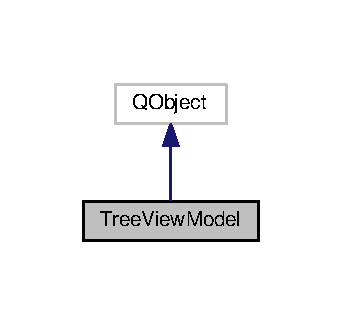
\includegraphics[width=164pt]{class_tree_view_model__inherit__graph}
\end{center}
\end{figure}


Collaboration diagram for Tree\+View\+Model\+:\nopagebreak
\begin{figure}[H]
\begin{center}
\leavevmode
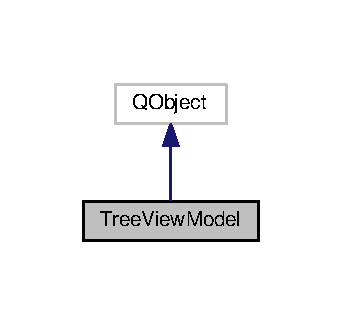
\includegraphics[width=164pt]{class_tree_view_model__coll__graph}
\end{center}
\end{figure}
\subsection*{Public Slots}
\begin{DoxyCompactItemize}
\item 
void \hyperlink{class_tree_view_model_ae3b9431925e42572a66aa51ae1ab785f}{update\+Name} (\hyperlink{class_projet}{Projet} $\ast$projet)
\begin{DoxyCompactList}\small\item\em Met à jour le nom d\textquotesingle{}un projet. \end{DoxyCompactList}\item 
void \hyperlink{class_tree_view_model_a20c0d80c255910d92ad4fac40cb3295f}{update\+Name} (\hyperlink{class_unitaire}{Unitaire} $\ast$tache)
\begin{DoxyCompactList}\small\item\em Met à jour le nom d\textquotesingle{}une tache unitaire. \end{DoxyCompactList}\item 
void \hyperlink{class_tree_view_model_a3958b72bf354014f1f233072902b5da8}{update\+Name} (\hyperlink{class_composite}{Composite} $\ast$tache)
\begin{DoxyCompactList}\small\item\em Met à jour le nom d\textquotesingle{}une tache composite. \end{DoxyCompactList}\end{DoxyCompactItemize}
\subsection*{Public Member Functions}
\begin{DoxyCompactItemize}
\item 
Q\+Standard\+Item\+Model $\ast$ \hyperlink{class_tree_view_model_af5e7f6992ae03a0c27130430b3c753f4}{get\+Modele} ()
\begin{DoxyCompactList}\small\item\em Retourne une référence sur le modèle du Tree\+View. \end{DoxyCompactList}\item 
void \hyperlink{class_tree_view_model_ac373475bea94e84c15588628f8e140d2}{print\+Tree} ()
\begin{DoxyCompactList}\small\item\em Affiche l\textquotesingle{}arbre complet au lancement de l\textquotesingle{}application. \end{DoxyCompactList}\item 
void \hyperlink{class_tree_view_model_ad7c89e0477e9da08cf71e73d023e3155}{add\+Projet} (\hyperlink{class_projet}{Projet} $\ast$nouveau\+Projet)
\begin{DoxyCompactList}\small\item\em Ajoute un projet à la racine (virtuelle) de l\textquotesingle{}arbre à l\textquotesingle{}ajout d\textquotesingle{}un projet. \end{DoxyCompactList}\item 
void \hyperlink{class_tree_view_model_a0e4a0fd3f762ca89591914494b0b8abd}{add\+Tache} (\hyperlink{class_projet}{Projet} $\ast$projet, \hyperlink{class_tache}{Tache} $\ast$tache)
\begin{DoxyCompactList}\small\item\em Ajoute une tache à un projet. \end{DoxyCompactList}\item 
void \hyperlink{class_tree_view_model_a3b36fb846f9bb7753fcf2d8e04b99bad}{add\+Tache} (\hyperlink{class_tache}{Tache} $\ast$tache\+Mere, \hyperlink{class_tache}{Tache} $\ast$tache)
\begin{DoxyCompactList}\small\item\em Ajoute une tache à une tache mère (composite) \end{DoxyCompactList}\item 
\hyperlink{class_tache}{Tache} $\ast$ \hyperlink{class_tree_view_model_ac036b65c8296ff50d616c06e5a9decfa}{get\+Tache\+From\+Item} (Q\+Standard\+Item $\ast$item)
\begin{DoxyCompactList}\small\item\em Retourne une tache à partir d\textquotesingle{}un item de l\textquotesingle{}arbre. \end{DoxyCompactList}\item 
Q\+Standard\+Item $\ast$ \hyperlink{class_tree_view_model_a71b5e1fb4a72adc756b6611b34a3a000}{get\+Item\+From\+Tache} (\hyperlink{class_tache}{Tache} $\ast$tache)
\begin{DoxyCompactList}\small\item\em Retourne l\textquotesingle{}item de l\textquotesingle{}arbre lié à une tache. \end{DoxyCompactList}\item 
\hyperlink{class_projet}{Projet} $\ast$ \hyperlink{class_tree_view_model_a1afea15d08be67340fff49476ddd3182}{get\+Projet\+From\+Item} (Q\+Standard\+Item $\ast$item)
\begin{DoxyCompactList}\small\item\em Retourne un projet à partir d\textquotesingle{}un item de l\textquotesingle{}arbre. \end{DoxyCompactList}\item 
Q\+Standard\+Item $\ast$ \hyperlink{class_tree_view_model_a54f066c26fef522024cd39f1eaf1c236}{get\+Item\+From\+Projet} (\hyperlink{class_projet}{Projet} $\ast$projet)
\begin{DoxyCompactList}\small\item\em Retourne l\textquotesingle{}item associé à un projet. \end{DoxyCompactList}\item 
void \hyperlink{class_tree_view_model_a9d049539995bcd46a98b58d0eb14f9b5}{update\+Icons} (\hyperlink{class_tache}{Tache} $\ast$t)
\begin{DoxyCompactList}\small\item\em Met à jour les icones de la tache t et de ses parents (quand une tache est programmée) \end{DoxyCompactList}\end{DoxyCompactItemize}
\subsection*{Static Public Member Functions}
\begin{DoxyCompactItemize}
\item 
static \hyperlink{class_tree_view_model}{Tree\+View\+Model} \& \hyperlink{class_tree_view_model_a46c11bb283dec5498dc096bde83006b7}{get\+Instance} ()
\begin{DoxyCompactList}\small\item\em Retourne l\textquotesingle{}instance de la classe. \end{DoxyCompactList}\item 
static void \hyperlink{class_tree_view_model_a263f6bd7971d922ea536fdedcbf6bb1b}{liberer\+Instance} ()
\end{DoxyCompactItemize}


\subsection{Detailed Description}
Gestionnaire singloton du modèle du Tree\+View~\newline
 

Contient les différentes méthodes afin d\textquotesingle{}afficher l\textquotesingle{}arbre des projets et taches.~\newline
 On connait ainsi les taches incluses dans un projet, et celles qui sont dans une tache composite.~\newline
 On voit rapidement l\textquotesingle{}état des taches/projet grace à une petite icone.~\newline
 Permet de retrouver un projet/tache à partir d\textquotesingle{}un item et inversement.~\newline
 

\subsection{Member Function Documentation}
\hypertarget{class_tree_view_model_ad7c89e0477e9da08cf71e73d023e3155}{}\index{Tree\+View\+Model@{Tree\+View\+Model}!add\+Projet@{add\+Projet}}
\index{add\+Projet@{add\+Projet}!Tree\+View\+Model@{Tree\+View\+Model}}
\subsubsection[{add\+Projet}]{\setlength{\rightskip}{0pt plus 5cm}void Tree\+View\+Model\+::add\+Projet (
\begin{DoxyParamCaption}
\item[{{\bf Projet} $\ast$}]{nouveau\+Projet}
\end{DoxyParamCaption}
)}\label{class_tree_view_model_ad7c89e0477e9da08cf71e73d023e3155}


Ajoute un projet à la racine (virtuelle) de l\textquotesingle{}arbre à l\textquotesingle{}ajout d\textquotesingle{}un projet. 

\hypertarget{class_tree_view_model_a0e4a0fd3f762ca89591914494b0b8abd}{}\index{Tree\+View\+Model@{Tree\+View\+Model}!add\+Tache@{add\+Tache}}
\index{add\+Tache@{add\+Tache}!Tree\+View\+Model@{Tree\+View\+Model}}
\subsubsection[{add\+Tache}]{\setlength{\rightskip}{0pt plus 5cm}void Tree\+View\+Model\+::add\+Tache (
\begin{DoxyParamCaption}
\item[{{\bf Projet} $\ast$}]{projet, }
\item[{{\bf Tache} $\ast$}]{tache}
\end{DoxyParamCaption}
)}\label{class_tree_view_model_a0e4a0fd3f762ca89591914494b0b8abd}


Ajoute une tache à un projet. 

\hypertarget{class_tree_view_model_a3b36fb846f9bb7753fcf2d8e04b99bad}{}\index{Tree\+View\+Model@{Tree\+View\+Model}!add\+Tache@{add\+Tache}}
\index{add\+Tache@{add\+Tache}!Tree\+View\+Model@{Tree\+View\+Model}}
\subsubsection[{add\+Tache}]{\setlength{\rightskip}{0pt plus 5cm}void Tree\+View\+Model\+::add\+Tache (
\begin{DoxyParamCaption}
\item[{{\bf Tache} $\ast$}]{tache\+Mere, }
\item[{{\bf Tache} $\ast$}]{tache}
\end{DoxyParamCaption}
)}\label{class_tree_view_model_a3b36fb846f9bb7753fcf2d8e04b99bad}


Ajoute une tache à une tache mère (composite) 

\hypertarget{class_tree_view_model_a46c11bb283dec5498dc096bde83006b7}{}\index{Tree\+View\+Model@{Tree\+View\+Model}!get\+Instance@{get\+Instance}}
\index{get\+Instance@{get\+Instance}!Tree\+View\+Model@{Tree\+View\+Model}}
\subsubsection[{get\+Instance}]{\setlength{\rightskip}{0pt plus 5cm}{\bf Tree\+View\+Model} \& Tree\+View\+Model\+::get\+Instance (
\begin{DoxyParamCaption}
{}
\end{DoxyParamCaption}
)\hspace{0.3cm}{\ttfamily [static]}}\label{class_tree_view_model_a46c11bb283dec5498dc096bde83006b7}


Retourne l\textquotesingle{}instance de la classe. 

\hypertarget{class_tree_view_model_a54f066c26fef522024cd39f1eaf1c236}{}\index{Tree\+View\+Model@{Tree\+View\+Model}!get\+Item\+From\+Projet@{get\+Item\+From\+Projet}}
\index{get\+Item\+From\+Projet@{get\+Item\+From\+Projet}!Tree\+View\+Model@{Tree\+View\+Model}}
\subsubsection[{get\+Item\+From\+Projet}]{\setlength{\rightskip}{0pt plus 5cm}Q\+Standard\+Item $\ast$ Tree\+View\+Model\+::get\+Item\+From\+Projet (
\begin{DoxyParamCaption}
\item[{{\bf Projet} $\ast$}]{projet}
\end{DoxyParamCaption}
)}\label{class_tree_view_model_a54f066c26fef522024cd39f1eaf1c236}


Retourne l\textquotesingle{}item associé à un projet. 

\hypertarget{class_tree_view_model_a71b5e1fb4a72adc756b6611b34a3a000}{}\index{Tree\+View\+Model@{Tree\+View\+Model}!get\+Item\+From\+Tache@{get\+Item\+From\+Tache}}
\index{get\+Item\+From\+Tache@{get\+Item\+From\+Tache}!Tree\+View\+Model@{Tree\+View\+Model}}
\subsubsection[{get\+Item\+From\+Tache}]{\setlength{\rightskip}{0pt plus 5cm}Q\+Standard\+Item $\ast$ Tree\+View\+Model\+::get\+Item\+From\+Tache (
\begin{DoxyParamCaption}
\item[{{\bf Tache} $\ast$}]{tache}
\end{DoxyParamCaption}
)}\label{class_tree_view_model_a71b5e1fb4a72adc756b6611b34a3a000}


Retourne l\textquotesingle{}item de l\textquotesingle{}arbre lié à une tache. 

\hypertarget{class_tree_view_model_af5e7f6992ae03a0c27130430b3c753f4}{}\index{Tree\+View\+Model@{Tree\+View\+Model}!get\+Modele@{get\+Modele}}
\index{get\+Modele@{get\+Modele}!Tree\+View\+Model@{Tree\+View\+Model}}
\subsubsection[{get\+Modele}]{\setlength{\rightskip}{0pt plus 5cm}Q\+Standard\+Item\+Model$\ast$ Tree\+View\+Model\+::get\+Modele (
\begin{DoxyParamCaption}
{}
\end{DoxyParamCaption}
)\hspace{0.3cm}{\ttfamily [inline]}}\label{class_tree_view_model_af5e7f6992ae03a0c27130430b3c753f4}


Retourne une référence sur le modèle du Tree\+View. 

\hypertarget{class_tree_view_model_a1afea15d08be67340fff49476ddd3182}{}\index{Tree\+View\+Model@{Tree\+View\+Model}!get\+Projet\+From\+Item@{get\+Projet\+From\+Item}}
\index{get\+Projet\+From\+Item@{get\+Projet\+From\+Item}!Tree\+View\+Model@{Tree\+View\+Model}}
\subsubsection[{get\+Projet\+From\+Item}]{\setlength{\rightskip}{0pt plus 5cm}{\bf Projet} $\ast$ Tree\+View\+Model\+::get\+Projet\+From\+Item (
\begin{DoxyParamCaption}
\item[{Q\+Standard\+Item $\ast$}]{item}
\end{DoxyParamCaption}
)}\label{class_tree_view_model_a1afea15d08be67340fff49476ddd3182}


Retourne un projet à partir d\textquotesingle{}un item de l\textquotesingle{}arbre. 

\hypertarget{class_tree_view_model_ac036b65c8296ff50d616c06e5a9decfa}{}\index{Tree\+View\+Model@{Tree\+View\+Model}!get\+Tache\+From\+Item@{get\+Tache\+From\+Item}}
\index{get\+Tache\+From\+Item@{get\+Tache\+From\+Item}!Tree\+View\+Model@{Tree\+View\+Model}}
\subsubsection[{get\+Tache\+From\+Item}]{\setlength{\rightskip}{0pt plus 5cm}{\bf Tache} $\ast$ Tree\+View\+Model\+::get\+Tache\+From\+Item (
\begin{DoxyParamCaption}
\item[{Q\+Standard\+Item $\ast$}]{item}
\end{DoxyParamCaption}
)}\label{class_tree_view_model_ac036b65c8296ff50d616c06e5a9decfa}


Retourne une tache à partir d\textquotesingle{}un item de l\textquotesingle{}arbre. 

\hypertarget{class_tree_view_model_a263f6bd7971d922ea536fdedcbf6bb1b}{}\index{Tree\+View\+Model@{Tree\+View\+Model}!liberer\+Instance@{liberer\+Instance}}
\index{liberer\+Instance@{liberer\+Instance}!Tree\+View\+Model@{Tree\+View\+Model}}
\subsubsection[{liberer\+Instance}]{\setlength{\rightskip}{0pt plus 5cm}void Tree\+View\+Model\+::liberer\+Instance (
\begin{DoxyParamCaption}
{}
\end{DoxyParamCaption}
)\hspace{0.3cm}{\ttfamily [static]}}\label{class_tree_view_model_a263f6bd7971d922ea536fdedcbf6bb1b}
\hypertarget{class_tree_view_model_ac373475bea94e84c15588628f8e140d2}{}\index{Tree\+View\+Model@{Tree\+View\+Model}!print\+Tree@{print\+Tree}}
\index{print\+Tree@{print\+Tree}!Tree\+View\+Model@{Tree\+View\+Model}}
\subsubsection[{print\+Tree}]{\setlength{\rightskip}{0pt plus 5cm}void Tree\+View\+Model\+::print\+Tree (
\begin{DoxyParamCaption}
{}
\end{DoxyParamCaption}
)}\label{class_tree_view_model_ac373475bea94e84c15588628f8e140d2}


Affiche l\textquotesingle{}arbre complet au lancement de l\textquotesingle{}application. 

\hypertarget{class_tree_view_model_a9d049539995bcd46a98b58d0eb14f9b5}{}\index{Tree\+View\+Model@{Tree\+View\+Model}!update\+Icons@{update\+Icons}}
\index{update\+Icons@{update\+Icons}!Tree\+View\+Model@{Tree\+View\+Model}}
\subsubsection[{update\+Icons}]{\setlength{\rightskip}{0pt plus 5cm}void Tree\+View\+Model\+::update\+Icons (
\begin{DoxyParamCaption}
\item[{{\bf Tache} $\ast$}]{t}
\end{DoxyParamCaption}
)}\label{class_tree_view_model_a9d049539995bcd46a98b58d0eb14f9b5}


Met à jour les icones de la tache t et de ses parents (quand une tache est programmée) 

\hypertarget{class_tree_view_model_ae3b9431925e42572a66aa51ae1ab785f}{}\index{Tree\+View\+Model@{Tree\+View\+Model}!update\+Name@{update\+Name}}
\index{update\+Name@{update\+Name}!Tree\+View\+Model@{Tree\+View\+Model}}
\subsubsection[{update\+Name}]{\setlength{\rightskip}{0pt plus 5cm}void Tree\+View\+Model\+::update\+Name (
\begin{DoxyParamCaption}
\item[{{\bf Projet} $\ast$}]{projet}
\end{DoxyParamCaption}
)\hspace{0.3cm}{\ttfamily [slot]}}\label{class_tree_view_model_ae3b9431925e42572a66aa51ae1ab785f}


Met à jour le nom d\textquotesingle{}un projet. 

\hypertarget{class_tree_view_model_a20c0d80c255910d92ad4fac40cb3295f}{}\index{Tree\+View\+Model@{Tree\+View\+Model}!update\+Name@{update\+Name}}
\index{update\+Name@{update\+Name}!Tree\+View\+Model@{Tree\+View\+Model}}
\subsubsection[{update\+Name}]{\setlength{\rightskip}{0pt plus 5cm}void Tree\+View\+Model\+::update\+Name (
\begin{DoxyParamCaption}
\item[{{\bf Unitaire} $\ast$}]{tache}
\end{DoxyParamCaption}
)\hspace{0.3cm}{\ttfamily [slot]}}\label{class_tree_view_model_a20c0d80c255910d92ad4fac40cb3295f}


Met à jour le nom d\textquotesingle{}une tache unitaire. 

\hypertarget{class_tree_view_model_a3958b72bf354014f1f233072902b5da8}{}\index{Tree\+View\+Model@{Tree\+View\+Model}!update\+Name@{update\+Name}}
\index{update\+Name@{update\+Name}!Tree\+View\+Model@{Tree\+View\+Model}}
\subsubsection[{update\+Name}]{\setlength{\rightskip}{0pt plus 5cm}void Tree\+View\+Model\+::update\+Name (
\begin{DoxyParamCaption}
\item[{{\bf Composite} $\ast$}]{tache}
\end{DoxyParamCaption}
)\hspace{0.3cm}{\ttfamily [slot]}}\label{class_tree_view_model_a3958b72bf354014f1f233072902b5da8}


Met à jour le nom d\textquotesingle{}une tache composite. 



The documentation for this class was generated from the following files\+:\begin{DoxyCompactItemize}
\item 
L\+O21app/\hyperlink{_u_i_classes_8h}{U\+I\+Classes.\+h}\item 
L\+O21app/\hyperlink{_u_i_classes_8cpp}{U\+I\+Classes.\+cpp}\end{DoxyCompactItemize}

\hypertarget{class_unitaire}{}\section{Unitaire Class Reference}
\label{class_unitaire}\index{Unitaire@{Unitaire}}


Classe de taches programmables, héritant de Tachet et d\textquotesingle{}\hyperlink{class_evenement}{Evenement} La classe de taches pouvant être programmées, en plusieurs fois si préemptive, en une seule fois sinon. La classe est forcément préemptive si sa durée dépasse 12h.  




{\ttfamily \#include $<$Calendar.\+h$>$}



Inheritance diagram for Unitaire\+:\nopagebreak
\begin{figure}[H]
\begin{center}
\leavevmode
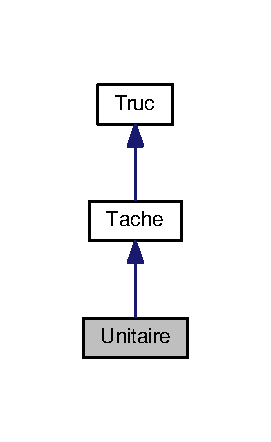
\includegraphics[width=208pt]{class_unitaire__inherit__graph}
\end{center}
\end{figure}


Collaboration diagram for Unitaire\+:\nopagebreak
\begin{figure}[H]
\begin{center}
\leavevmode
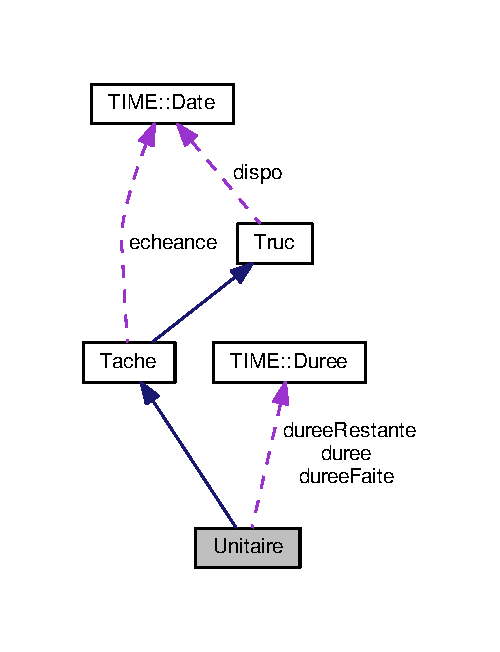
\includegraphics[width=208pt]{class_unitaire__coll__graph}
\end{center}
\end{figure}
\subsection*{Public Member Functions}
\begin{DoxyCompactItemize}
\item 
virtual void \hyperlink{class_unitaire_a804454c39eb010aa67bd622a009df840}{add\+Item} (\hyperlink{class_tache}{Tache} $\ast$t)
\begin{DoxyCompactList}\small\item\em Ajoute la tache pointée aux tableau de précédences prec. \end{DoxyCompactList}\item 
bool \hyperlink{class_unitaire_adba3a8de0fe6273cea7eecda3520bfcd}{is\+Preemp} () const 
\begin{DoxyCompactList}\small\item\em Indique si la tache est préemptable ou non. \end{DoxyCompactList}\item 
\hyperlink{class_t_i_m_e_1_1_duree}{Duree} \hyperlink{class_unitaire_a9ab243102aa0572048a956204532b201}{get\+Fait} () const 
\begin{DoxyCompactList}\small\item\em Retourne la durée faite de la tache. \end{DoxyCompactList}\item 
\hyperlink{class_t_i_m_e_1_1_duree}{Duree} \hyperlink{class_unitaire_a2fa3fa1073200a18c9a2706b37eb78e6}{get\+Restant} () const 
\begin{DoxyCompactList}\small\item\em Retourne la durée restante à programmer de la tache, calculée en soustrayant la durée totale avec la dutée faite. \end{DoxyCompactList}\item 
int \hyperlink{class_unitaire_aadf6c5718aff37f1a7589240059e9e98}{get\+Statut} ()
\begin{DoxyCompactList}\small\item\em Retourne le statut de la tache \+: 0 = rien n\textquotesingle{}est fait, 1 = en cours, 2 = terminé/deadline passée. \end{DoxyCompactList}\item 
virtual int \hyperlink{class_unitaire_affee1a6cda05a1032eba560196af99b9}{is\+Finished} (const \hyperlink{class_t_i_m_e_1_1_date}{Date} \&d, const \hyperlink{class_t_i_m_e_1_1_horaire}{Horaire} \&h)
\begin{DoxyCompactList}\small\item\em Renvoie 1 si la tache a été terminée à la date d et l\textquotesingle{}horaire h, 0 sinon. \end{DoxyCompactList}\item 
void \hyperlink{class_unitaire_ad9ef9d9bb2b47520c3c609d822364964}{set\+Fait} (const \hyperlink{class_t_i_m_e_1_1_duree}{Duree} \&f)
\begin{DoxyCompactList}\small\item\em Modifie la durée faite de la tache. \end{DoxyCompactList}\item 
void \hyperlink{class_unitaire_aa4893599f98385c26884441655331bc2}{set\+Preemp} ()
\begin{DoxyCompactList}\small\item\em Rend la tache préemptable. \end{DoxyCompactList}\item 
void \hyperlink{class_unitaire_a8bb9a65dc5b0d03a44353edfae06580d}{set\+Non\+Preemp} ()
\begin{DoxyCompactList}\small\item\em Rend, si possible, la tache preemptable. \end{DoxyCompactList}\item 
virtual void \hyperlink{class_unitaire_a98bd645b84e0bd2f378e13774324f7b7}{afficher} (ostream \&f)
\begin{DoxyCompactList}\small\item\em Affiche les attributs de la tache. \end{DoxyCompactList}\item 
void \hyperlink{class_unitaire_a965c3d4d8ba7864ae28a24a5d514dec5}{update} (string id, string t, \hyperlink{class_t_i_m_e_1_1_date}{Date} d, \hyperlink{class_t_i_m_e_1_1_date}{Date} e, \hyperlink{class_t_i_m_e_1_1_duree}{Duree} dur, \hyperlink{class_t_i_m_e_1_1_duree}{Duree} df, bool p)
\item 
void \hyperlink{class_unitaire_a2f189cf8c1bc7d22b805e6bfd1aa0bd7}{update} (string t, \hyperlink{class_t_i_m_e_1_1_date}{Date} d, \hyperlink{class_t_i_m_e_1_1_date}{Date} e, \hyperlink{class_t_i_m_e_1_1_duree}{Duree} dur, bool p)
\end{DoxyCompactItemize}
\subsection*{Friends}
\begin{DoxyCompactItemize}
\item 
\hyperlink{class_unitaire}{Unitaire} \& \hyperlink{class_unitaire_af32ab372e13abfb17b253ade6390cfd3}{Projet\+::ajouter\+Unitaire} (const string \&t, const \hyperlink{class_t_i_m_e_1_1_date}{Date} \&dispo, const \hyperlink{class_t_i_m_e_1_1_date}{Date} \&deadline, const \hyperlink{class_t_i_m_e_1_1_duree}{Duree} \&duree, const bool premp)
\end{DoxyCompactItemize}


\subsection{Detailed Description}
Classe de taches programmables, héritant de Tachet et d\textquotesingle{}\hyperlink{class_evenement}{Evenement} La classe de taches pouvant être programmées, en plusieurs fois si préemptive, en une seule fois sinon. La classe est forcément préemptive si sa durée dépasse 12h. 

\subsection{Member Function Documentation}
\hypertarget{class_unitaire_a804454c39eb010aa67bd622a009df840}{}\index{Unitaire@{Unitaire}!add\+Item@{add\+Item}}
\index{add\+Item@{add\+Item}!Unitaire@{Unitaire}}
\subsubsection[{add\+Item}]{\setlength{\rightskip}{0pt plus 5cm}virtual void Unitaire\+::add\+Item (
\begin{DoxyParamCaption}
\item[{{\bf Tache} $\ast$}]{t}
\end{DoxyParamCaption}
)\hspace{0.3cm}{\ttfamily [inline]}, {\ttfamily [virtual]}}\label{class_unitaire_a804454c39eb010aa67bd622a009df840}


Ajoute la tache pointée aux tableau de précédences prec. 



Reimplemented from \hyperlink{class_tache_a6a13b4138a46f22e632bf9d35f155c09}{Tache}.

\hypertarget{class_unitaire_a98bd645b84e0bd2f378e13774324f7b7}{}\index{Unitaire@{Unitaire}!afficher@{afficher}}
\index{afficher@{afficher}!Unitaire@{Unitaire}}
\subsubsection[{afficher}]{\setlength{\rightskip}{0pt plus 5cm}void Unitaire\+::afficher (
\begin{DoxyParamCaption}
\item[{ostream \&}]{f}
\end{DoxyParamCaption}
)\hspace{0.3cm}{\ttfamily [virtual]}}\label{class_unitaire_a98bd645b84e0bd2f378e13774324f7b7}


Affiche les attributs de la tache. 



Implements \hyperlink{class_evenement_af217f0cd3d421e3f113a13536ee63593}{Evenement}.

\hypertarget{class_unitaire_a9ab243102aa0572048a956204532b201}{}\index{Unitaire@{Unitaire}!get\+Fait@{get\+Fait}}
\index{get\+Fait@{get\+Fait}!Unitaire@{Unitaire}}
\subsubsection[{get\+Fait}]{\setlength{\rightskip}{0pt plus 5cm}{\bf Duree} Unitaire\+::get\+Fait (
\begin{DoxyParamCaption}
{}
\end{DoxyParamCaption}
) const\hspace{0.3cm}{\ttfamily [inline]}}\label{class_unitaire_a9ab243102aa0572048a956204532b201}


Retourne la durée faite de la tache. 

\hypertarget{class_unitaire_a2fa3fa1073200a18c9a2706b37eb78e6}{}\index{Unitaire@{Unitaire}!get\+Restant@{get\+Restant}}
\index{get\+Restant@{get\+Restant}!Unitaire@{Unitaire}}
\subsubsection[{get\+Restant}]{\setlength{\rightskip}{0pt plus 5cm}{\bf Duree} Unitaire\+::get\+Restant (
\begin{DoxyParamCaption}
{}
\end{DoxyParamCaption}
) const\hspace{0.3cm}{\ttfamily [inline]}}\label{class_unitaire_a2fa3fa1073200a18c9a2706b37eb78e6}


Retourne la durée restante à programmer de la tache, calculée en soustrayant la durée totale avec la dutée faite. 

\hypertarget{class_unitaire_aadf6c5718aff37f1a7589240059e9e98}{}\index{Unitaire@{Unitaire}!get\+Statut@{get\+Statut}}
\index{get\+Statut@{get\+Statut}!Unitaire@{Unitaire}}
\subsubsection[{get\+Statut}]{\setlength{\rightskip}{0pt plus 5cm}int Unitaire\+::get\+Statut (
\begin{DoxyParamCaption}
{}
\end{DoxyParamCaption}
)\hspace{0.3cm}{\ttfamily [virtual]}}\label{class_unitaire_aadf6c5718aff37f1a7589240059e9e98}


Retourne le statut de la tache \+: 0 = rien n\textquotesingle{}est fait, 1 = en cours, 2 = terminé/deadline passée. 



Implements \hyperlink{class_tache_ac60426a56aec80b995f30456fc60a256}{Tache}.

\hypertarget{class_unitaire_affee1a6cda05a1032eba560196af99b9}{}\index{Unitaire@{Unitaire}!is\+Finished@{is\+Finished}}
\index{is\+Finished@{is\+Finished}!Unitaire@{Unitaire}}
\subsubsection[{is\+Finished}]{\setlength{\rightskip}{0pt plus 5cm}int Unitaire\+::is\+Finished (
\begin{DoxyParamCaption}
\item[{const {\bf Date} \&}]{d, }
\item[{const {\bf Horaire} \&}]{h}
\end{DoxyParamCaption}
)\hspace{0.3cm}{\ttfamily [virtual]}}\label{class_unitaire_affee1a6cda05a1032eba560196af99b9}


Renvoie 1 si la tache a été terminée à la date d et l\textquotesingle{}horaire h, 0 sinon. 



Implements \hyperlink{class_tache_a495d9d787ef400a510e625e4e51014bd}{Tache}.

\hypertarget{class_unitaire_adba3a8de0fe6273cea7eecda3520bfcd}{}\index{Unitaire@{Unitaire}!is\+Preemp@{is\+Preemp}}
\index{is\+Preemp@{is\+Preemp}!Unitaire@{Unitaire}}
\subsubsection[{is\+Preemp}]{\setlength{\rightskip}{0pt plus 5cm}bool Unitaire\+::is\+Preemp (
\begin{DoxyParamCaption}
{}
\end{DoxyParamCaption}
) const\hspace{0.3cm}{\ttfamily [inline]}}\label{class_unitaire_adba3a8de0fe6273cea7eecda3520bfcd}


Indique si la tache est préemptable ou non. 

\hypertarget{class_unitaire_ad9ef9d9bb2b47520c3c609d822364964}{}\index{Unitaire@{Unitaire}!set\+Fait@{set\+Fait}}
\index{set\+Fait@{set\+Fait}!Unitaire@{Unitaire}}
\subsubsection[{set\+Fait}]{\setlength{\rightskip}{0pt plus 5cm}void Unitaire\+::set\+Fait (
\begin{DoxyParamCaption}
\item[{const {\bf Duree} \&}]{f}
\end{DoxyParamCaption}
)\hspace{0.3cm}{\ttfamily [inline]}}\label{class_unitaire_ad9ef9d9bb2b47520c3c609d822364964}


Modifie la durée faite de la tache. 

\hypertarget{class_unitaire_a8bb9a65dc5b0d03a44353edfae06580d}{}\index{Unitaire@{Unitaire}!set\+Non\+Preemp@{set\+Non\+Preemp}}
\index{set\+Non\+Preemp@{set\+Non\+Preemp}!Unitaire@{Unitaire}}
\subsubsection[{set\+Non\+Preemp}]{\setlength{\rightskip}{0pt plus 5cm}void Unitaire\+::set\+Non\+Preemp (
\begin{DoxyParamCaption}
{}
\end{DoxyParamCaption}
)\hspace{0.3cm}{\ttfamily [inline]}}\label{class_unitaire_a8bb9a65dc5b0d03a44353edfae06580d}


Rend, si possible, la tache preemptable. 

\hypertarget{class_unitaire_aa4893599f98385c26884441655331bc2}{}\index{Unitaire@{Unitaire}!set\+Preemp@{set\+Preemp}}
\index{set\+Preemp@{set\+Preemp}!Unitaire@{Unitaire}}
\subsubsection[{set\+Preemp}]{\setlength{\rightskip}{0pt plus 5cm}void Unitaire\+::set\+Preemp (
\begin{DoxyParamCaption}
{}
\end{DoxyParamCaption}
)\hspace{0.3cm}{\ttfamily [inline]}}\label{class_unitaire_aa4893599f98385c26884441655331bc2}


Rend la tache préemptable. 

\hypertarget{class_unitaire_a965c3d4d8ba7864ae28a24a5d514dec5}{}\index{Unitaire@{Unitaire}!update@{update}}
\index{update@{update}!Unitaire@{Unitaire}}
\subsubsection[{update}]{\setlength{\rightskip}{0pt plus 5cm}void Unitaire\+::update (
\begin{DoxyParamCaption}
\item[{string}]{id, }
\item[{string}]{t, }
\item[{{\bf Date}}]{d, }
\item[{{\bf Date}}]{e, }
\item[{{\bf Duree}}]{dur, }
\item[{{\bf Duree}}]{df, }
\item[{bool}]{p}
\end{DoxyParamCaption}
)\hspace{0.3cm}{\ttfamily [inline]}}\label{class_unitaire_a965c3d4d8ba7864ae28a24a5d514dec5}
Met à jour la tache en modifiant ses attributs à partir des paramètres donnés \+: id, titre, disponibilité, échéance, durée, durée faite et préemptabilité \hypertarget{class_unitaire_a2f189cf8c1bc7d22b805e6bfd1aa0bd7}{}\index{Unitaire@{Unitaire}!update@{update}}
\index{update@{update}!Unitaire@{Unitaire}}
\subsubsection[{update}]{\setlength{\rightskip}{0pt plus 5cm}void Unitaire\+::update (
\begin{DoxyParamCaption}
\item[{string}]{t, }
\item[{{\bf Date}}]{d, }
\item[{{\bf Date}}]{e, }
\item[{{\bf Duree}}]{dur, }
\item[{bool}]{p}
\end{DoxyParamCaption}
)\hspace{0.3cm}{\ttfamily [inline]}}\label{class_unitaire_a2f189cf8c1bc7d22b805e6bfd1aa0bd7}
Met à jour la tache en modifiant ses attributs à partir des paramètres donnés \+: id, titre, disponibilité, échéance, durée et préemptabilité 

\subsection{Friends And Related Function Documentation}
\hypertarget{class_unitaire_af32ab372e13abfb17b253ade6390cfd3}{}\index{Unitaire@{Unitaire}!Projet\+::ajouter\+Unitaire@{Projet\+::ajouter\+Unitaire}}
\index{Projet\+::ajouter\+Unitaire@{Projet\+::ajouter\+Unitaire}!Unitaire@{Unitaire}}
\subsubsection[{Projet\+::ajouter\+Unitaire}]{\setlength{\rightskip}{0pt plus 5cm}{\bf Unitaire}\& {\bf Projet\+::ajouter\+Unitaire} (
\begin{DoxyParamCaption}
\item[{const string \&}]{t, }
\item[{const {\bf Date} \&}]{dispo, }
\item[{const {\bf Date} \&}]{deadline, }
\item[{const {\bf Duree} \&}]{duree, }
\item[{const bool}]{premp}
\end{DoxyParamCaption}
)\hspace{0.3cm}{\ttfamily [friend]}}\label{class_unitaire_af32ab372e13abfb17b253ade6390cfd3}


The documentation for this class was generated from the following files\+:\begin{DoxyCompactItemize}
\item 
L\+O21app/\hyperlink{_calendar_8h}{Calendar.\+h}\item 
L\+O21app/\hyperlink{_calendar_8cpp}{Calendar.\+cpp}\end{DoxyCompactItemize}

\chapter{File Documentation}
\hypertarget{agendaview_8cpp}{}\section{L\+O21app/agendaview.cpp File Reference}
\label{agendaview_8cpp}\index{L\+O21app/agendaview.\+cpp@{L\+O21app/agendaview.\+cpp}}
{\ttfamily \#include \char`\"{}agendaview.\+h\char`\"{}}\\*
{\ttfamily \#include \char`\"{}ui\+\_\+agendaview.\+h\char`\"{}}\\*
Include dependency graph for agendaview.\+cpp\+:\nopagebreak
\begin{figure}[H]
\begin{center}
\leavevmode
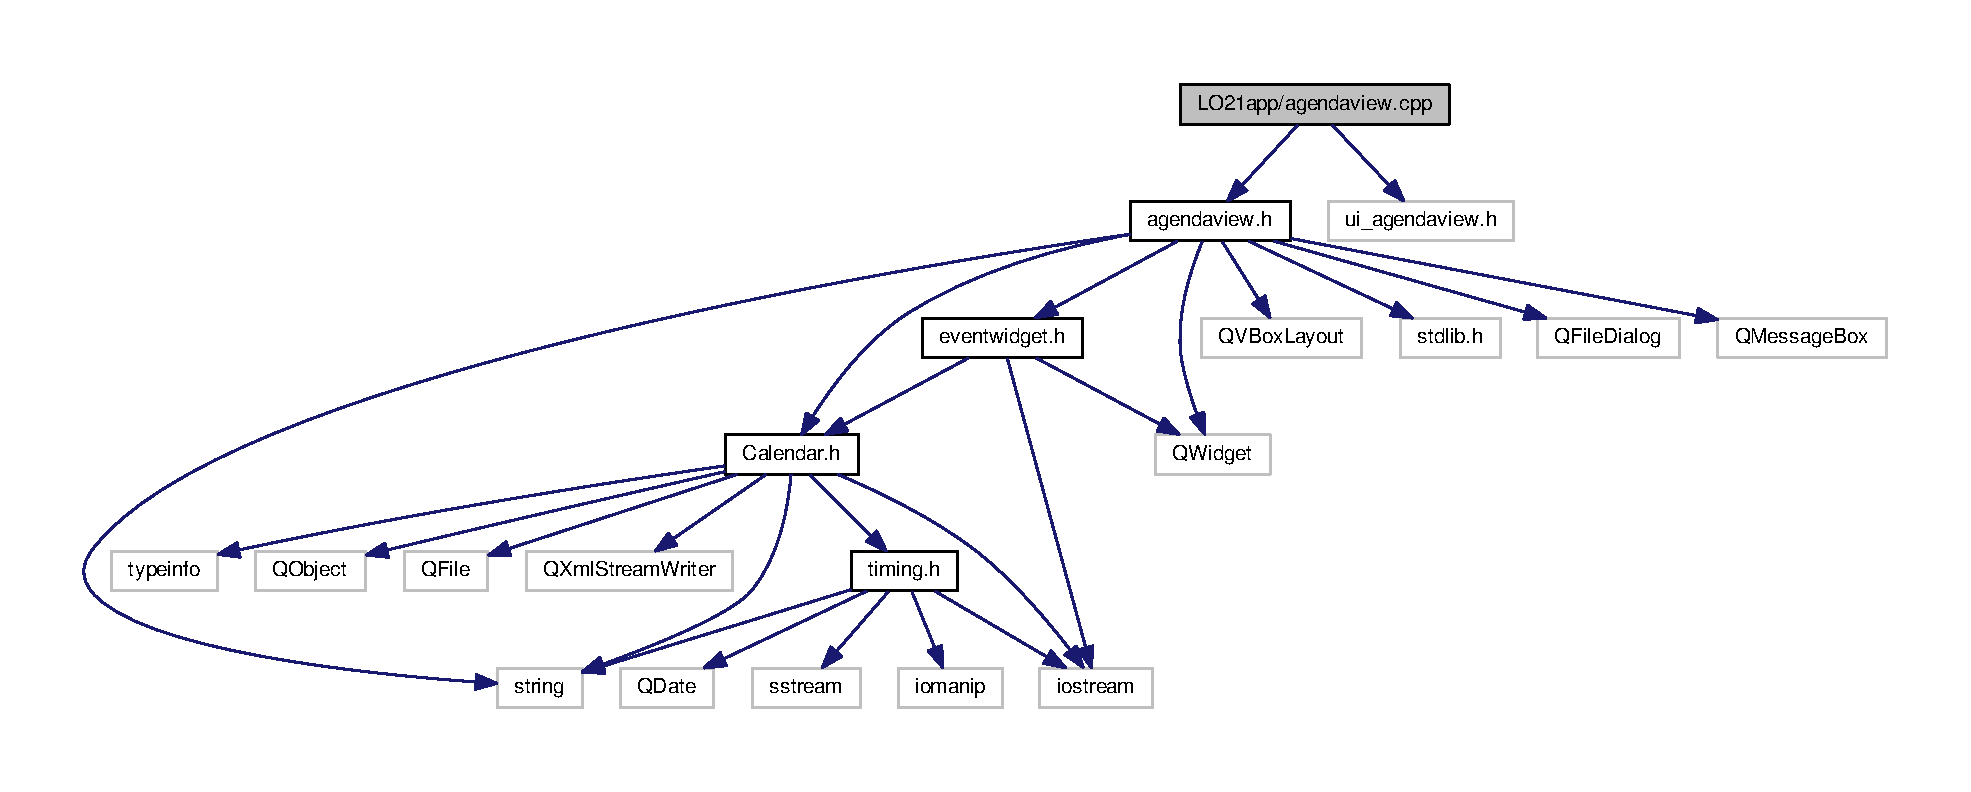
\includegraphics[width=350pt]{agendaview_8cpp__incl}
\end{center}
\end{figure}

\hypertarget{agendaview_8h}{}\section{L\+O21app/agendaview.h File Reference}
\label{agendaview_8h}\index{L\+O21app/agendaview.\+h@{L\+O21app/agendaview.\+h}}
{\ttfamily \#include \char`\"{}Calendar.\+h\char`\"{}}\\*
{\ttfamily \#include \char`\"{}eventwidget.\+h\char`\"{}}\\*
{\ttfamily \#include $<$Q\+Widget$>$}\\*
{\ttfamily \#include $<$Q\+V\+Box\+Layout$>$}\\*
{\ttfamily \#include $<$stdlib.\+h$>$}\\*
{\ttfamily \#include $<$string$>$}\\*
{\ttfamily \#include $<$Q\+File\+Dialog$>$}\\*
{\ttfamily \#include $<$Q\+Message\+Box$>$}\\*
Include dependency graph for agendaview.\+h\+:\nopagebreak
\begin{figure}[H]
\begin{center}
\leavevmode
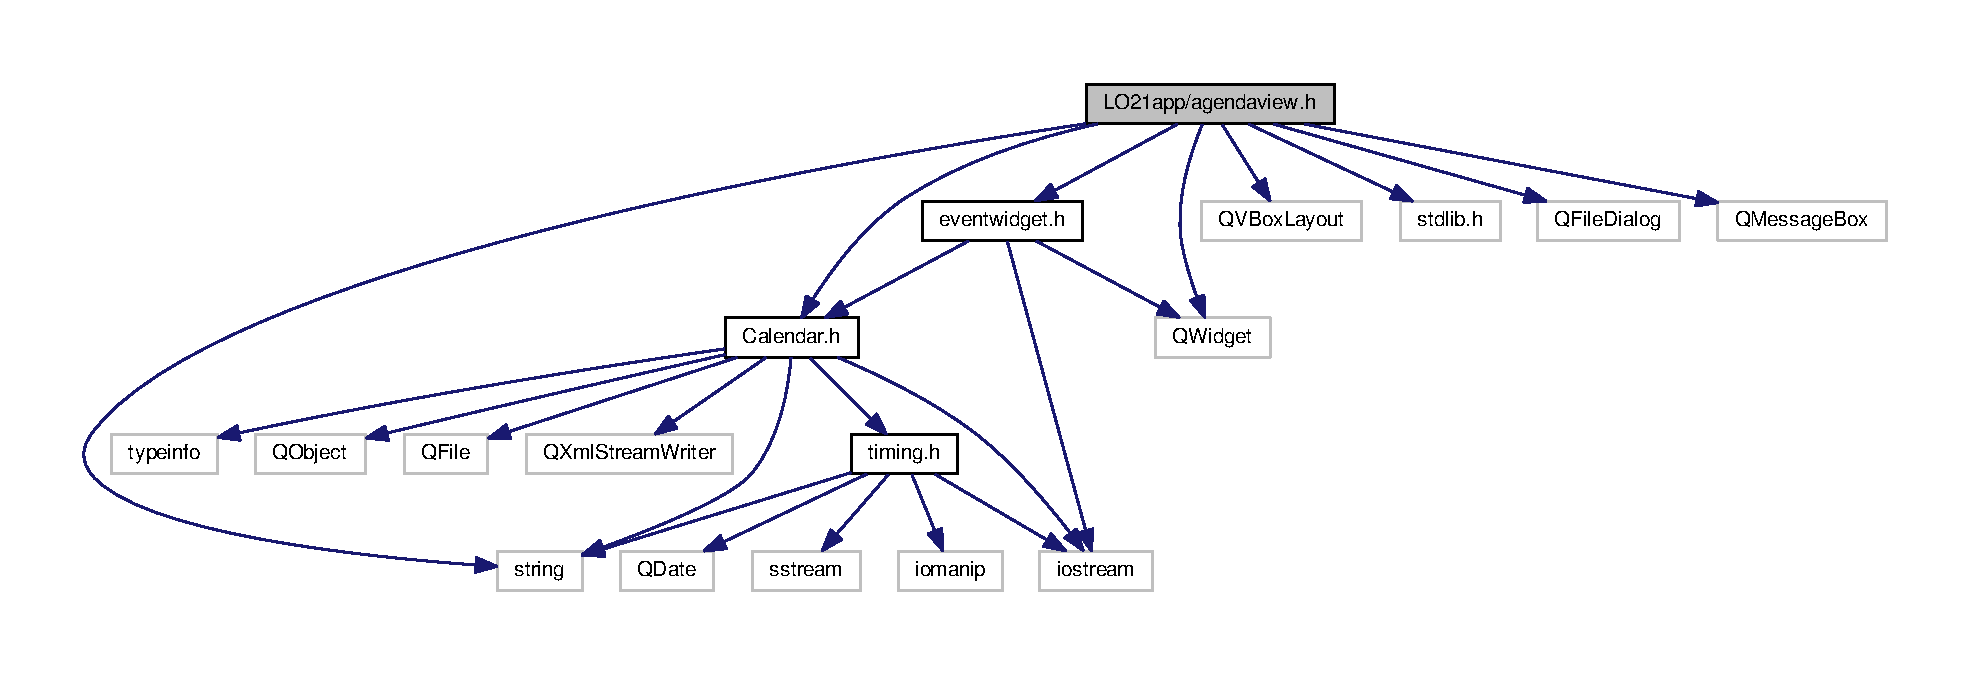
\includegraphics[width=350pt]{agendaview_8h__incl}
\end{center}
\end{figure}
This graph shows which files directly or indirectly include this file\+:\nopagebreak
\begin{figure}[H]
\begin{center}
\leavevmode
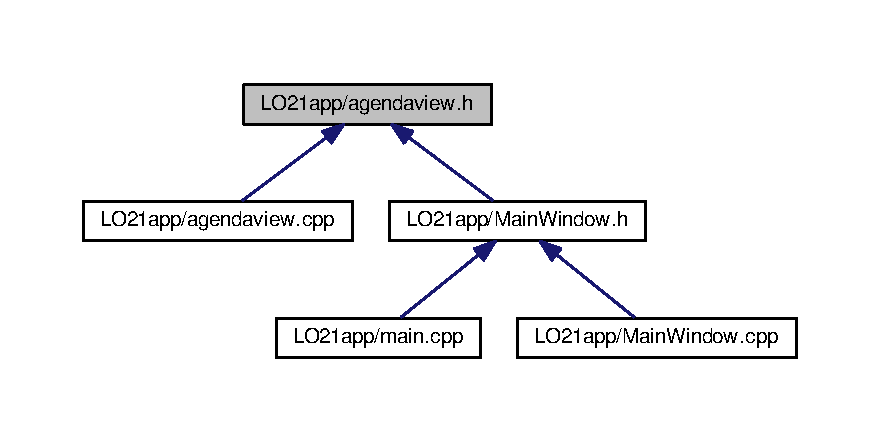
\includegraphics[width=350pt]{agendaview_8h__dep__incl}
\end{center}
\end{figure}
\subsection*{Classes}
\begin{DoxyCompactItemize}
\item 
class \hyperlink{class_agenda_view}{Agenda\+View}
\begin{DoxyCompactList}\small\item\em Classe d\textquotesingle{}U\+I gérant le contenu de l\textquotesingle{}onglet Agenda. \end{DoxyCompactList}\end{DoxyCompactItemize}
\subsection*{Namespaces}
\begin{DoxyCompactItemize}
\item 
 \hyperlink{namespace_ui}{Ui}
\end{DoxyCompactItemize}

\hypertarget{_calendar_8cpp}{}\section{L\+O21app/\+Calendar.cpp File Reference}
\label{_calendar_8cpp}\index{L\+O21app/\+Calendar.\+cpp@{L\+O21app/\+Calendar.\+cpp}}
{\ttfamily \#include \char`\"{}Calendar.\+h\char`\"{}}\\*
{\ttfamily \#include $<$fstream$>$}\\*
Include dependency graph for Calendar.\+cpp\+:\nopagebreak
\begin{figure}[H]
\begin{center}
\leavevmode
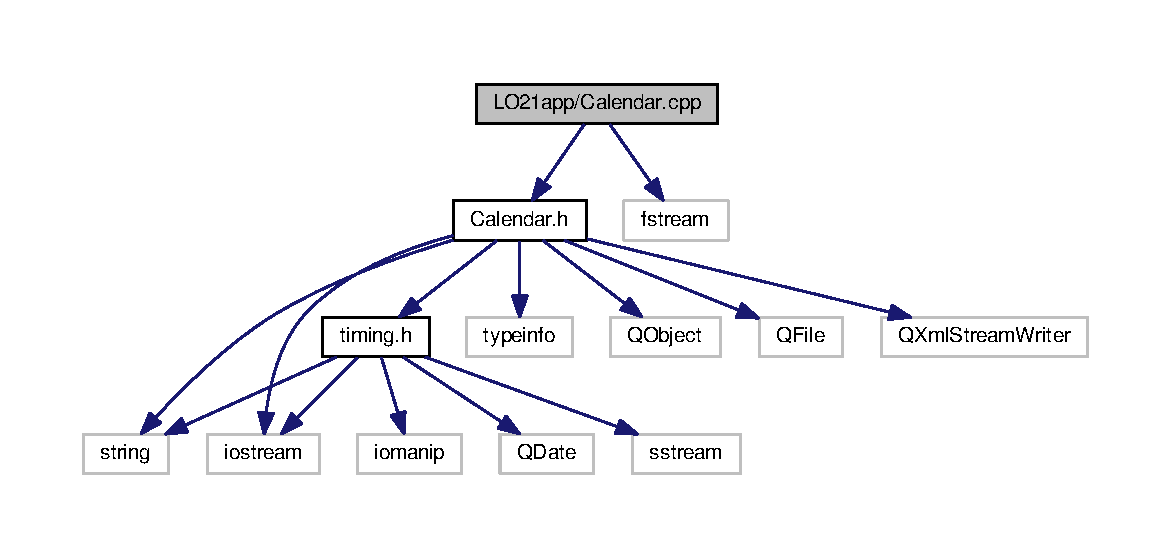
\includegraphics[width=350pt]{_calendar_8cpp__incl}
\end{center}
\end{figure}
\subsection*{Functions}
\begin{DoxyCompactItemize}
\item 
ostream \& \hyperlink{_calendar_8cpp_a0dba4e6aa6c43b21abb115f7d77ab61d}{operator$<$$<$} (ostream \&fout, \hyperlink{class_tache}{Tache} \&t)
\end{DoxyCompactItemize}


\subsection{Function Documentation}
\hypertarget{_calendar_8cpp_a0dba4e6aa6c43b21abb115f7d77ab61d}{}\index{Calendar.\+cpp@{Calendar.\+cpp}!operator$<$$<$@{operator$<$$<$}}
\index{operator$<$$<$@{operator$<$$<$}!Calendar.\+cpp@{Calendar.\+cpp}}
\subsubsection[{operator$<$$<$}]{\setlength{\rightskip}{0pt plus 5cm}ostream\& operator$<$$<$ (
\begin{DoxyParamCaption}
\item[{ostream \&}]{fout, }
\item[{{\bf Tache} \&}]{t}
\end{DoxyParamCaption}
)}\label{_calendar_8cpp_a0dba4e6aa6c43b21abb115f7d77ab61d}

\hypertarget{_calendar_8h}{}\section{L\+O21app/\+Calendar.h File Reference}
\label{_calendar_8h}\index{L\+O21app/\+Calendar.\+h@{L\+O21app/\+Calendar.\+h}}
{\ttfamily \#include $<$string$>$}\\*
{\ttfamily \#include $<$iostream$>$}\\*
{\ttfamily \#include $<$typeinfo$>$}\\*
{\ttfamily \#include $<$Q\+Object$>$}\\*
{\ttfamily \#include $<$Q\+File$>$}\\*
{\ttfamily \#include $<$Q\+Xml\+Stream\+Writer$>$}\\*
{\ttfamily \#include \char`\"{}timing.\+h\char`\"{}}\\*
Include dependency graph for Calendar.\+h\+:\nopagebreak
\begin{figure}[H]
\begin{center}
\leavevmode
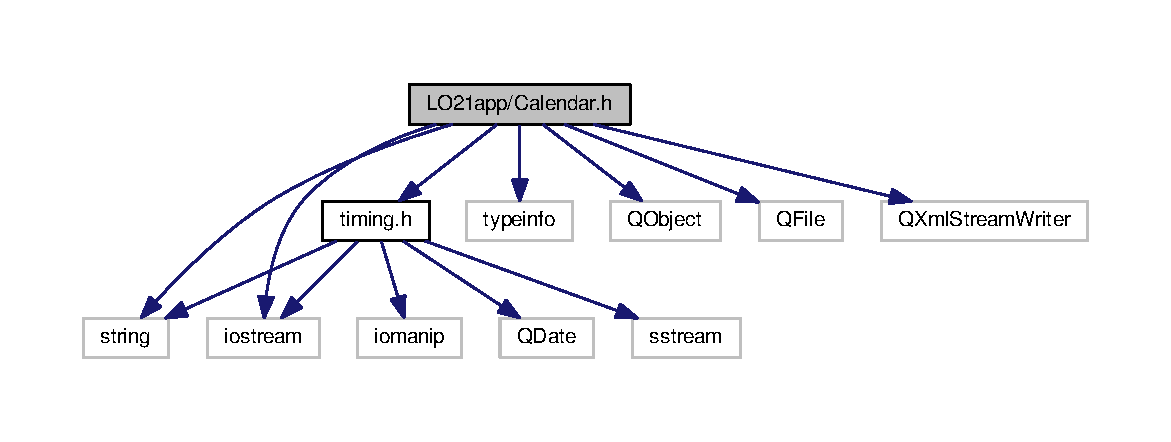
\includegraphics[width=350pt]{_calendar_8h__incl}
\end{center}
\end{figure}
This graph shows which files directly or indirectly include this file\+:\nopagebreak
\begin{figure}[H]
\begin{center}
\leavevmode
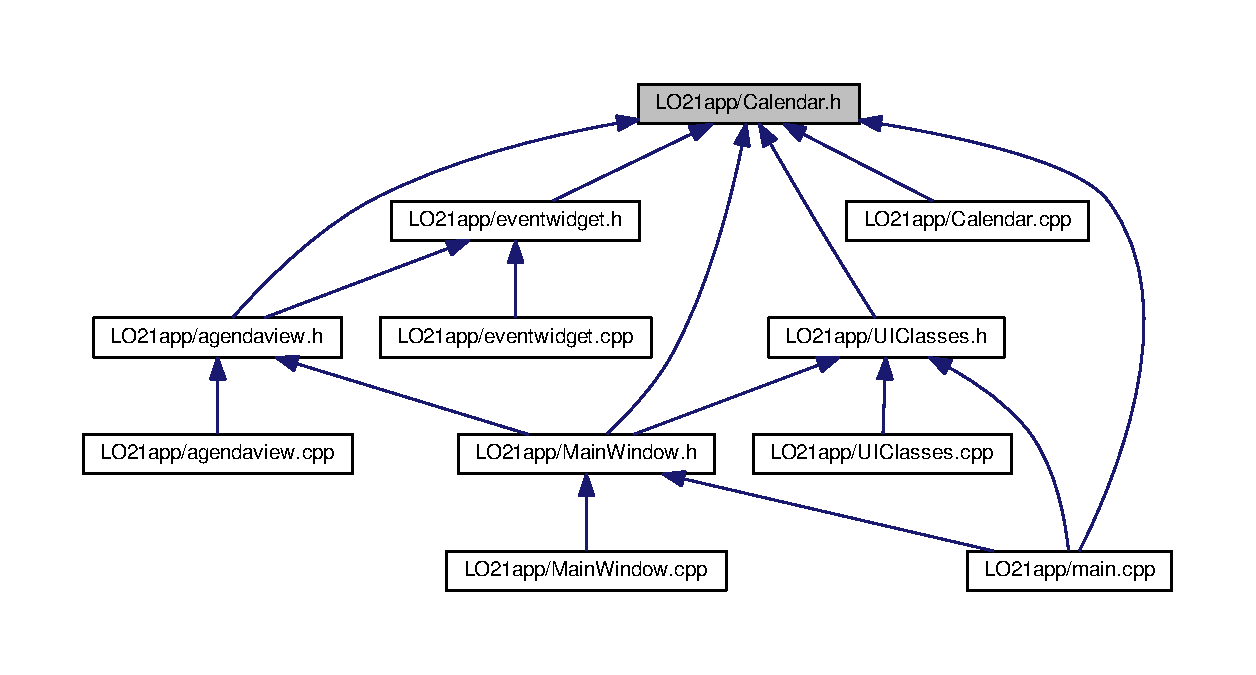
\includegraphics[width=350pt]{_calendar_8h__dep__incl}
\end{center}
\end{figure}
\subsection*{Classes}
\begin{DoxyCompactItemize}
\item 
class \hyperlink{class_calendar_exception}{Calendar\+Exception}
\begin{DoxyCompactList}\small\item\em Classe permettant de gérer les exceptions du projet non liées au namespace \hyperlink{namespace_t_i_m_e}{T\+I\+M\+E}. \end{DoxyCompactList}\item 
class \hyperlink{class_projet_manager}{Projet\+Manager}
\begin{DoxyCompactList}\small\item\em Classe composite des Projets La classe applique le designe pattern singleton et possède un iterateur sur le tableau de pointeurs de Projets. \end{DoxyCompactList}\item 
class \hyperlink{class_projet_manager_1_1_iterator}{Projet\+Manager\+::\+Iterator}
\item 
class \hyperlink{class_projet}{Projet}
\begin{DoxyCompactList}\small\item\em Classe de projets composite des Taches et composant \hyperlink{class_projet_manager}{Projet\+Manager}. \end{DoxyCompactList}\item 
class \hyperlink{class_projet_1_1_iterator}{Projet\+::\+Iterator}
\item 
class \hyperlink{class_evenement}{Evenement}
\begin{DoxyCompactList}\small\item\em Classe abstraite d\textquotesingle{}éléments pouvant être programmés. \end{DoxyCompactList}\item 
class \hyperlink{class_tache}{Tache}
\begin{DoxyCompactList}\small\item\em Classe abstraite de taches composant \hyperlink{class_projet}{Projet}. \end{DoxyCompactList}\item 
class \hyperlink{class_tache_1_1_iterator}{Tache\+::\+Iterator}
\item 
class \hyperlink{class_unitaire}{Unitaire}
\begin{DoxyCompactList}\small\item\em Classe de taches programmables, héritant de Tachet et d\textquotesingle{}\hyperlink{class_evenement}{Evenement} La classe de taches pouvant être programmées, en plusieurs fois si préemptive, en une seule fois sinon. La classe est forcément préemptive si sa durée dépasse 12h. \end{DoxyCompactList}\item 
class \hyperlink{class_composite}{Composite}
\begin{DoxyCompactList}\small\item\em Classe d\textquotesingle{}ensembles de taches, héritant de \hyperlink{class_tache}{Tache} La classe possède un pointeur de Taches qui représente les composants de la tache composite. \end{DoxyCompactList}\item 
class \hyperlink{class_composite_1_1_compo_iterator}{Composite\+::\+Compo\+Iterator}
\item 
class \hyperlink{class_activite}{Activite}
\begin{DoxyCompactList}\small\item\em Classe d\textquotesingle{}evenement basique programmable, héritant d\textquotesingle{}\hyperlink{class_evenement}{Evenement} La classe possède un titre et un lieu. \end{DoxyCompactList}\item 
class \hyperlink{class_programmation_manager}{Programmation\+Manager}
\begin{DoxyCompactList}\small\item\em Classe composite de \hyperlink{class_programmation}{Programmation} La classe applique le designe pattern singleton et possède un iterateur sur le tableau de pointeurs de Programmations. \end{DoxyCompactList}\item 
class \hyperlink{class_programmation_manager_1_1_iterator}{Programmation\+Manager\+::\+Iterator}
\item 
class \hyperlink{class_programmation}{Programmation}
\begin{DoxyCompactList}\small\item\em Classe donnant une date, un horaire et une durée à une \hyperlink{class_evenement}{Evenement}, classe composant \hyperlink{class_programmation_manager}{Programmation\+Manager}. \end{DoxyCompactList}\end{DoxyCompactItemize}
\subsection*{Functions}
\begin{DoxyCompactItemize}
\item 
ostream \& \hyperlink{_calendar_8h_a0f16d28c485a5fc98a0f07b53d6009b1}{operator$<$$<$} (ostream \&f, const \hyperlink{class_tache}{Tache} \&t)
\begin{DoxyCompactList}\small\item\em Operator d\textquotesingle{}affichage de \hyperlink{class_tache}{Tache} sur un ostream. \end{DoxyCompactList}\end{DoxyCompactItemize}


\subsection{Function Documentation}
\hypertarget{_calendar_8h_a0f16d28c485a5fc98a0f07b53d6009b1}{}\index{Calendar.\+h@{Calendar.\+h}!operator$<$$<$@{operator$<$$<$}}
\index{operator$<$$<$@{operator$<$$<$}!Calendar.\+h@{Calendar.\+h}}
\subsubsection[{operator$<$$<$}]{\setlength{\rightskip}{0pt plus 5cm}ostream\& operator$<$$<$ (
\begin{DoxyParamCaption}
\item[{ostream \&}]{f, }
\item[{const {\bf Tache} \&}]{t}
\end{DoxyParamCaption}
)}\label{_calendar_8h_a0f16d28c485a5fc98a0f07b53d6009b1}


Operator d\textquotesingle{}affichage de \hyperlink{class_tache}{Tache} sur un ostream. 


\hypertarget{eventwidget_8cpp}{}\section{L\+O21app/eventwidget.cpp File Reference}
\label{eventwidget_8cpp}\index{L\+O21app/eventwidget.\+cpp@{L\+O21app/eventwidget.\+cpp}}
{\ttfamily \#include \char`\"{}eventwidget.\+h\char`\"{}}\\*
{\ttfamily \#include \char`\"{}ui\+\_\+eventwidget.\+h\char`\"{}}\\*
Include dependency graph for eventwidget.\+cpp\+:\nopagebreak
\begin{figure}[H]
\begin{center}
\leavevmode
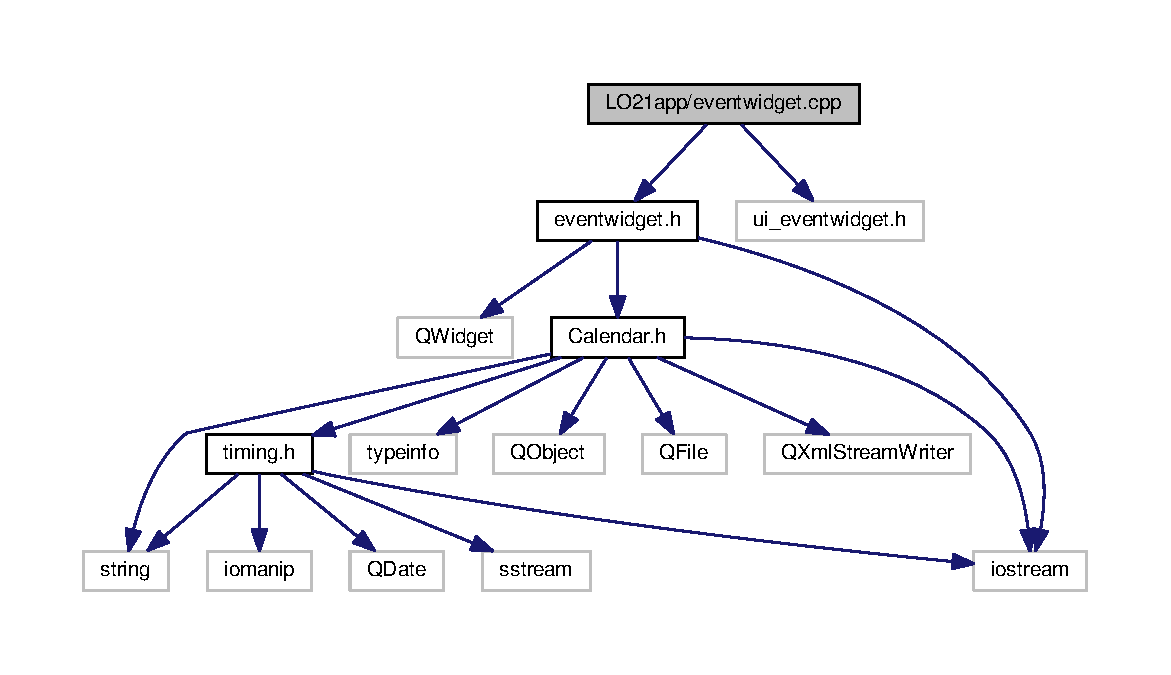
\includegraphics[width=350pt]{eventwidget_8cpp__incl}
\end{center}
\end{figure}

\hypertarget{eventwidget_8h}{}\section{L\+O21app/eventwidget.h File Reference}
\label{eventwidget_8h}\index{L\+O21app/eventwidget.\+h@{L\+O21app/eventwidget.\+h}}
{\ttfamily \#include $<$Q\+Widget$>$}\\*
{\ttfamily \#include $<$iostream$>$}\\*
{\ttfamily \#include \char`\"{}Calendar.\+h\char`\"{}}\\*
Include dependency graph for eventwidget.\+h\+:\nopagebreak
\begin{figure}[H]
\begin{center}
\leavevmode
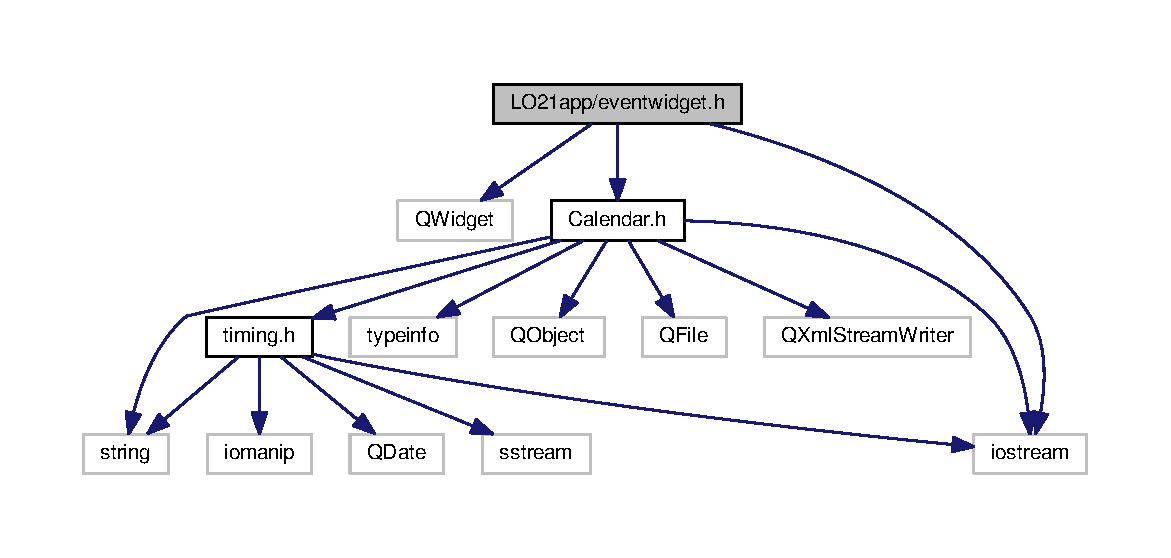
\includegraphics[width=350pt]{eventwidget_8h__incl}
\end{center}
\end{figure}
This graph shows which files directly or indirectly include this file\+:\nopagebreak
\begin{figure}[H]
\begin{center}
\leavevmode
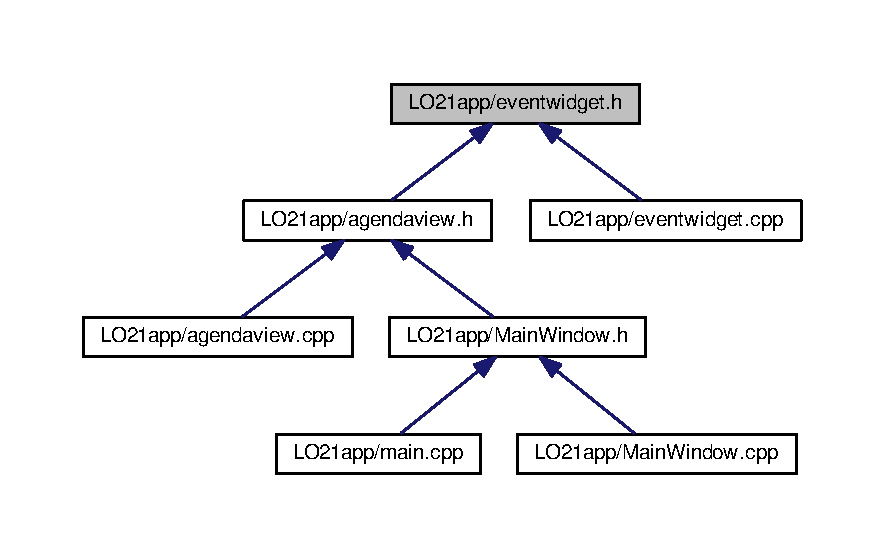
\includegraphics[width=350pt]{eventwidget_8h__dep__incl}
\end{center}
\end{figure}
\subsection*{Classes}
\begin{DoxyCompactItemize}
\item 
class \hyperlink{class_event_widget}{Event\+Widget}
\begin{DoxyCompactList}\small\item\em Classe U\+I affichant un évènement dans l\textquotesingle{}agenda. \end{DoxyCompactList}\end{DoxyCompactItemize}
\subsection*{Namespaces}
\begin{DoxyCompactItemize}
\item 
 \hyperlink{namespace_ui}{Ui}
\end{DoxyCompactItemize}

\hypertarget{main_8cpp}{}\section{L\+O21app/main.cpp File Reference}
\label{main_8cpp}\index{L\+O21app/main.\+cpp@{L\+O21app/main.\+cpp}}
{\ttfamily \#include \char`\"{}Main\+Window.\+h\char`\"{}}\\*
{\ttfamily \#include $<$Q\+Application$>$}\\*
{\ttfamily \#include \char`\"{}Calendar.\+h\char`\"{}}\\*
{\ttfamily \#include \char`\"{}U\+I\+Classes.\+h\char`\"{}}\\*
Include dependency graph for main.\+cpp\+:\nopagebreak
\begin{figure}[H]
\begin{center}
\leavevmode
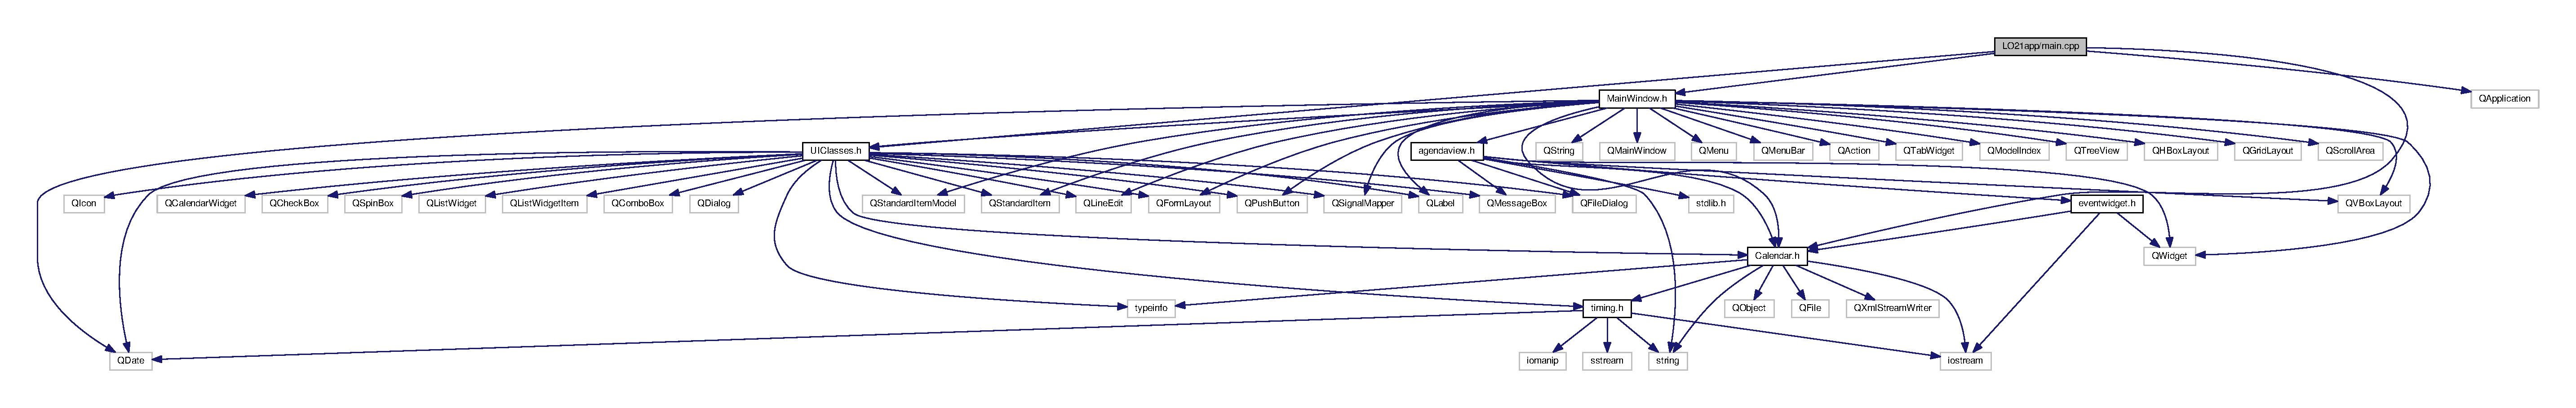
\includegraphics[width=350pt]{main_8cpp__incl}
\end{center}
\end{figure}
\subsection*{Functions}
\begin{DoxyCompactItemize}
\item 
int \hyperlink{main_8cpp_a0ddf1224851353fc92bfbff6f499fa97}{main} (int argc, char $\ast$argv\mbox{[}$\,$\mbox{]})
\end{DoxyCompactItemize}


\subsection{Function Documentation}
\hypertarget{main_8cpp_a0ddf1224851353fc92bfbff6f499fa97}{}\index{main.\+cpp@{main.\+cpp}!main@{main}}
\index{main@{main}!main.\+cpp@{main.\+cpp}}
\subsubsection[{main}]{\setlength{\rightskip}{0pt plus 5cm}int main (
\begin{DoxyParamCaption}
\item[{int}]{argc, }
\item[{char $\ast$}]{argv\mbox{[}$\,$\mbox{]}}
\end{DoxyParamCaption}
)}\label{main_8cpp_a0ddf1224851353fc92bfbff6f499fa97}

\hypertarget{_main_window_8cpp}{}\section{L\+O21app/\+Main\+Window.cpp File Reference}
\label{_main_window_8cpp}\index{L\+O21app/\+Main\+Window.\+cpp@{L\+O21app/\+Main\+Window.\+cpp}}
{\ttfamily \#include \char`\"{}Main\+Window.\+h\char`\"{}}\\*
Include dependency graph for Main\+Window.\+cpp\+:\nopagebreak
\begin{figure}[H]
\begin{center}
\leavevmode
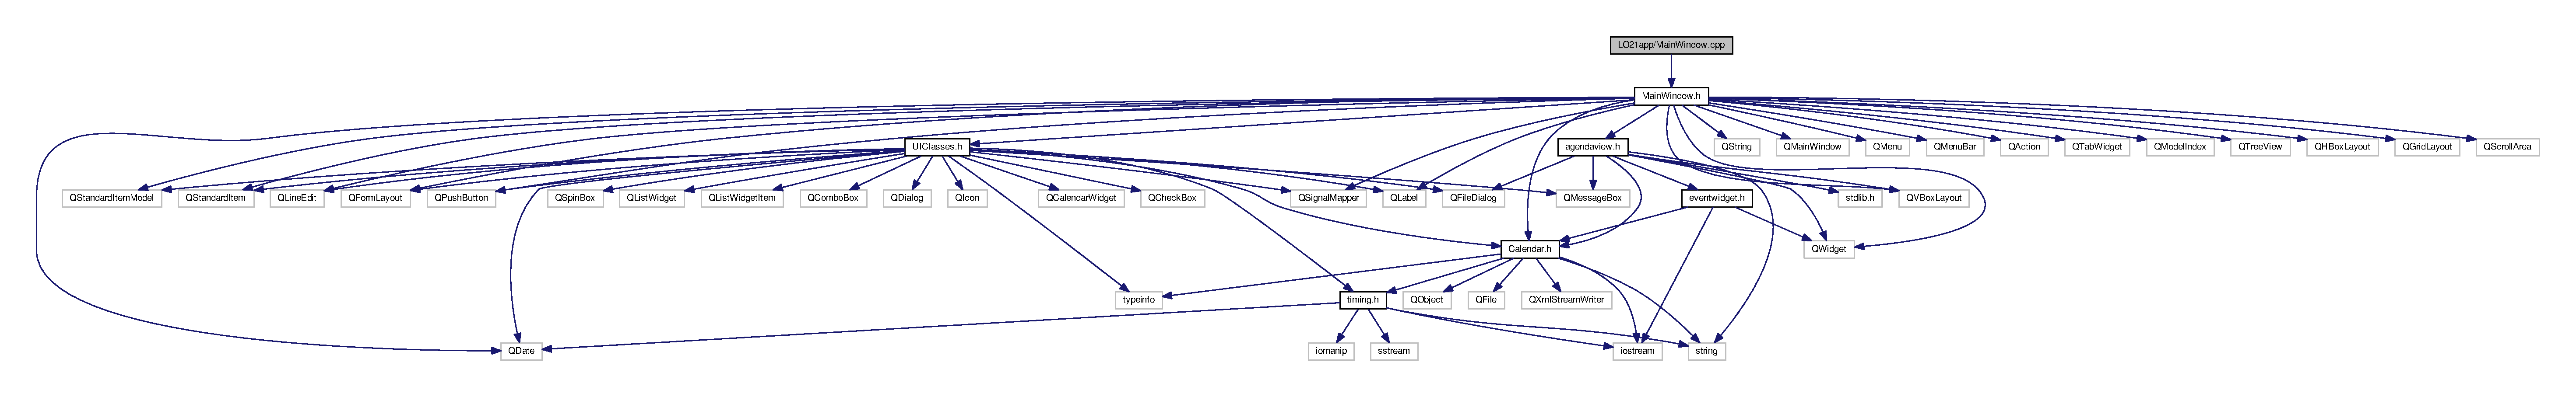
\includegraphics[width=350pt]{_main_window_8cpp__incl}
\end{center}
\end{figure}

\hypertarget{_main_window_8h}{}\section{L\+O21app/\+Main\+Window.h File Reference}
\label{_main_window_8h}\index{L\+O21app/\+Main\+Window.\+h@{L\+O21app/\+Main\+Window.\+h}}
{\ttfamily \#include \char`\"{}Calendar.\+h\char`\"{}}\\*
{\ttfamily \#include \char`\"{}U\+I\+Classes.\+h\char`\"{}}\\*
{\ttfamily \#include \char`\"{}agendaview.\+h\char`\"{}}\\*
{\ttfamily \#include $<$Q\+String$>$}\\*
{\ttfamily \#include $<$Q\+Main\+Window$>$}\\*
{\ttfamily \#include $<$Q\+Widget$>$}\\*
{\ttfamily \#include $<$Q\+Menu$>$}\\*
{\ttfamily \#include $<$Q\+Menu\+Bar$>$}\\*
{\ttfamily \#include $<$Q\+Action$>$}\\*
{\ttfamily \#include $<$Q\+Tab\+Widget$>$}\\*
{\ttfamily \#include $<$Q\+Standard\+Item\+Model$>$}\\*
{\ttfamily \#include $<$Q\+Standard\+Item$>$}\\*
{\ttfamily \#include $<$Q\+Model\+Index$>$}\\*
{\ttfamily \#include $<$Q\+Tree\+View$>$}\\*
{\ttfamily \#include $<$Q\+Form\+Layout$>$}\\*
{\ttfamily \#include $<$Q\+Line\+Edit$>$}\\*
{\ttfamily \#include $<$Q\+H\+Box\+Layout$>$}\\*
{\ttfamily \#include $<$Q\+V\+Box\+Layout$>$}\\*
{\ttfamily \#include $<$Q\+Date$>$}\\*
{\ttfamily \#include $<$Q\+Push\+Button$>$}\\*
{\ttfamily \#include $<$Q\+Grid\+Layout$>$}\\*
{\ttfamily \#include $<$Q\+Label$>$}\\*
{\ttfamily \#include $<$Q\+Signal\+Mapper$>$}\\*
{\ttfamily \#include $<$Q\+Scroll\+Area$>$}\\*
Include dependency graph for Main\+Window.\+h\+:\nopagebreak
\begin{figure}[H]
\begin{center}
\leavevmode
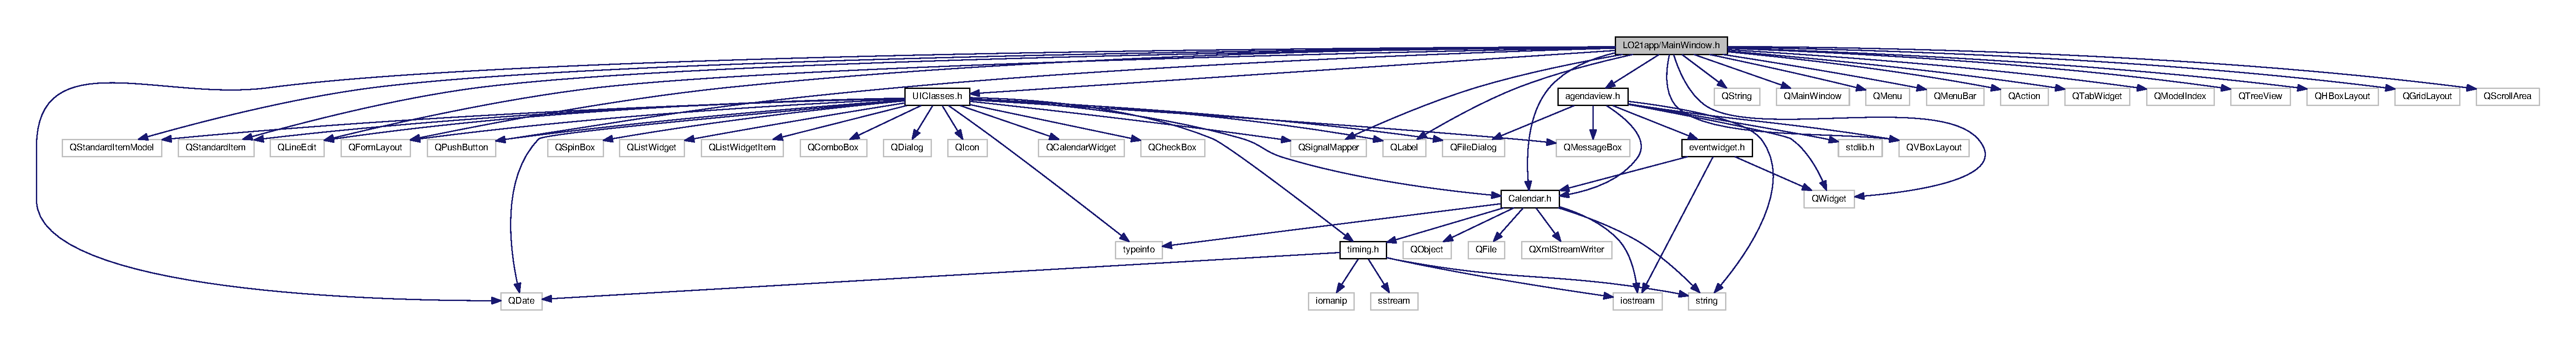
\includegraphics[width=350pt]{_main_window_8h__incl}
\end{center}
\end{figure}
This graph shows which files directly or indirectly include this file\+:\nopagebreak
\begin{figure}[H]
\begin{center}
\leavevmode
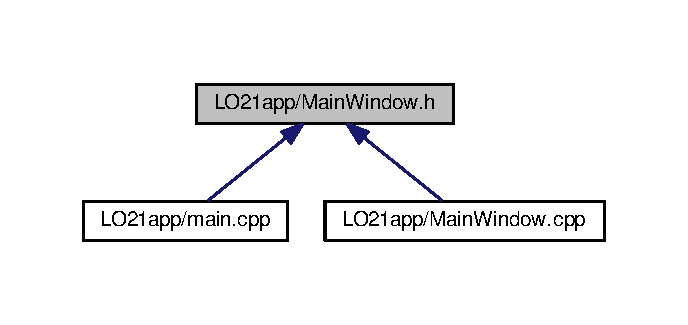
\includegraphics[width=330pt]{_main_window_8h__dep__incl}
\end{center}
\end{figure}
\subsection*{Classes}
\begin{DoxyCompactItemize}
\item 
class \hyperlink{class_main_window}{Main\+Window}
\begin{DoxyCompactList}\small\item\em Conserve les pointeurs vers les principaux widgets de la fenêtre. S\textquotesingle{}occupe des actions générales sur ceux-\/ci. \end{DoxyCompactList}\end{DoxyCompactItemize}
\subsection*{Macros}
\begin{DoxyCompactItemize}
\item 
\#define \hyperlink{_main_window_8h_a921a8595db82694a0ed9992b9dce1399}{W\+\_\+\+W\+I\+D\+T\+H}~1100
\item 
\#define \hyperlink{_main_window_8h_a0bb30e7a160522a2b0f55d44929bf4eb}{W\+\_\+\+H\+E\+I\+G\+H\+T}~700
\end{DoxyCompactItemize}


\subsection{Macro Definition Documentation}
\hypertarget{_main_window_8h_a0bb30e7a160522a2b0f55d44929bf4eb}{}\index{Main\+Window.\+h@{Main\+Window.\+h}!W\+\_\+\+H\+E\+I\+G\+H\+T@{W\+\_\+\+H\+E\+I\+G\+H\+T}}
\index{W\+\_\+\+H\+E\+I\+G\+H\+T@{W\+\_\+\+H\+E\+I\+G\+H\+T}!Main\+Window.\+h@{Main\+Window.\+h}}
\subsubsection[{W\+\_\+\+H\+E\+I\+G\+H\+T}]{\setlength{\rightskip}{0pt plus 5cm}\#define W\+\_\+\+H\+E\+I\+G\+H\+T~700}\label{_main_window_8h_a0bb30e7a160522a2b0f55d44929bf4eb}
\hypertarget{_main_window_8h_a921a8595db82694a0ed9992b9dce1399}{}\index{Main\+Window.\+h@{Main\+Window.\+h}!W\+\_\+\+W\+I\+D\+T\+H@{W\+\_\+\+W\+I\+D\+T\+H}}
\index{W\+\_\+\+W\+I\+D\+T\+H@{W\+\_\+\+W\+I\+D\+T\+H}!Main\+Window.\+h@{Main\+Window.\+h}}
\subsubsection[{W\+\_\+\+W\+I\+D\+T\+H}]{\setlength{\rightskip}{0pt plus 5cm}\#define W\+\_\+\+W\+I\+D\+T\+H~1100}\label{_main_window_8h_a921a8595db82694a0ed9992b9dce1399}

\hypertarget{timing_8cpp}{}\section{L\+O21app/timing.cpp File Reference}
\label{timing_8cpp}\index{L\+O21app/timing.\+cpp@{L\+O21app/timing.\+cpp}}
{\ttfamily \#include $<$iomanip$>$}\\*
{\ttfamily \#include \char`\"{}timing.\+h\char`\"{}}\\*
{\ttfamily \#include $<$ctime$>$}\\*
Include dependency graph for timing.\+cpp\+:\nopagebreak
\begin{figure}[H]
\begin{center}
\leavevmode
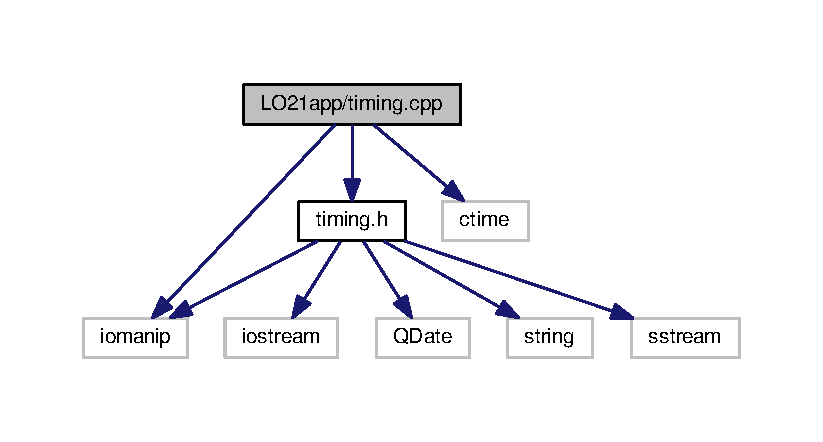
\includegraphics[width=350pt]{timing_8cpp__incl}
\end{center}
\end{figure}
\subsection*{Functions}
\begin{DoxyCompactItemize}
\item 
std\+::ostream \& \hyperlink{timing_8cpp_a61023d1614a8f824531248e65477b011}{operator$<$$<$} (std\+::ostream \&f, const \hyperlink{class_t_i_m_e_1_1_date}{Date} \&x)
\item 
std\+::ostream \& \hyperlink{timing_8cpp_a6284a7363d6d2ce972a91942a16b4d35}{operator$<$$<$} (std\+::ostream \&f, const \hyperlink{class_t_i_m_e_1_1_duree}{Duree} \&d)
\item 
std\+::ostream \& \hyperlink{timing_8cpp_ab8bcb53e2f89144d47fb96dc04025af6}{operator$<$$<$} (std\+::ostream \&f, const \hyperlink{class_t_i_m_e_1_1_horaire}{Horaire} \&h)
\item 
std\+::ostream \& \hyperlink{timing_8cpp_a7c5e1668e7b14f4e4f920a8c1f0c1517}{operator$<$$<$} (std\+::ostream \&f, const \hyperlink{class_t_i_m_e_1_1_periode}{Periode} \&p)
\item 
std\+::ostream \& \hyperlink{timing_8cpp_a4a74fe56c6c1e3e9219b264d7cfb57fb}{operator$<$$<$} (std\+::ostream \&f, const \hyperlink{class_t_i_m_e_1_1_intervalle}{Intervalle} \&x)
\item 
std\+::istream \& \hyperlink{timing_8cpp_a362506a09f2fabcb2165e40f4ad5dfeb}{operator$>$$>$} (std\+::istream \&flot, \hyperlink{class_t_i_m_e_1_1_date}{T\+I\+M\+E\+::\+Date} \&date)
\item 
std\+::istream \& \hyperlink{timing_8cpp_ad409b0b312aeec4effe00284be8f718c}{operator$>$$>$} (std\+::istream \&flot, \hyperlink{class_t_i_m_e_1_1_duree}{T\+I\+M\+E\+::\+Duree} \&duree)
\end{DoxyCompactItemize}


\subsection{Function Documentation}
\hypertarget{timing_8cpp_a61023d1614a8f824531248e65477b011}{}\index{timing.\+cpp@{timing.\+cpp}!operator$<$$<$@{operator$<$$<$}}
\index{operator$<$$<$@{operator$<$$<$}!timing.\+cpp@{timing.\+cpp}}
\subsubsection[{operator$<$$<$}]{\setlength{\rightskip}{0pt plus 5cm}std\+::ostream\& operator$<$$<$ (
\begin{DoxyParamCaption}
\item[{std\+::ostream \&}]{f, }
\item[{const {\bf Date} \&}]{x}
\end{DoxyParamCaption}
)}\label{timing_8cpp_a61023d1614a8f824531248e65477b011}
\hypertarget{timing_8cpp_a6284a7363d6d2ce972a91942a16b4d35}{}\index{timing.\+cpp@{timing.\+cpp}!operator$<$$<$@{operator$<$$<$}}
\index{operator$<$$<$@{operator$<$$<$}!timing.\+cpp@{timing.\+cpp}}
\subsubsection[{operator$<$$<$}]{\setlength{\rightskip}{0pt plus 5cm}std\+::ostream\& operator$<$$<$ (
\begin{DoxyParamCaption}
\item[{std\+::ostream \&}]{f, }
\item[{const {\bf Duree} \&}]{d}
\end{DoxyParamCaption}
)}\label{timing_8cpp_a6284a7363d6d2ce972a91942a16b4d35}
\hypertarget{timing_8cpp_ab8bcb53e2f89144d47fb96dc04025af6}{}\index{timing.\+cpp@{timing.\+cpp}!operator$<$$<$@{operator$<$$<$}}
\index{operator$<$$<$@{operator$<$$<$}!timing.\+cpp@{timing.\+cpp}}
\subsubsection[{operator$<$$<$}]{\setlength{\rightskip}{0pt plus 5cm}std\+::ostream\& operator$<$$<$ (
\begin{DoxyParamCaption}
\item[{std\+::ostream \&}]{f, }
\item[{const {\bf Horaire} \&}]{h}
\end{DoxyParamCaption}
)}\label{timing_8cpp_ab8bcb53e2f89144d47fb96dc04025af6}
\hypertarget{timing_8cpp_a7c5e1668e7b14f4e4f920a8c1f0c1517}{}\index{timing.\+cpp@{timing.\+cpp}!operator$<$$<$@{operator$<$$<$}}
\index{operator$<$$<$@{operator$<$$<$}!timing.\+cpp@{timing.\+cpp}}
\subsubsection[{operator$<$$<$}]{\setlength{\rightskip}{0pt plus 5cm}std\+::ostream\& operator$<$$<$ (
\begin{DoxyParamCaption}
\item[{std\+::ostream \&}]{f, }
\item[{const {\bf Periode} \&}]{p}
\end{DoxyParamCaption}
)}\label{timing_8cpp_a7c5e1668e7b14f4e4f920a8c1f0c1517}
\hypertarget{timing_8cpp_a4a74fe56c6c1e3e9219b264d7cfb57fb}{}\index{timing.\+cpp@{timing.\+cpp}!operator$<$$<$@{operator$<$$<$}}
\index{operator$<$$<$@{operator$<$$<$}!timing.\+cpp@{timing.\+cpp}}
\subsubsection[{operator$<$$<$}]{\setlength{\rightskip}{0pt plus 5cm}std\+::ostream\& operator$<$$<$ (
\begin{DoxyParamCaption}
\item[{std\+::ostream \&}]{f, }
\item[{const {\bf Intervalle} \&}]{x}
\end{DoxyParamCaption}
)}\label{timing_8cpp_a4a74fe56c6c1e3e9219b264d7cfb57fb}
\hypertarget{timing_8cpp_a362506a09f2fabcb2165e40f4ad5dfeb}{}\index{timing.\+cpp@{timing.\+cpp}!operator$>$$>$@{operator$>$$>$}}
\index{operator$>$$>$@{operator$>$$>$}!timing.\+cpp@{timing.\+cpp}}
\subsubsection[{operator$>$$>$}]{\setlength{\rightskip}{0pt plus 5cm}std\+::istream\& operator$>$$>$ (
\begin{DoxyParamCaption}
\item[{std\+::istream \&}]{flot, }
\item[{{\bf T\+I\+M\+E\+::\+Date} \&}]{date}
\end{DoxyParamCaption}
)}\label{timing_8cpp_a362506a09f2fabcb2165e40f4ad5dfeb}
\hypertarget{timing_8cpp_ad409b0b312aeec4effe00284be8f718c}{}\index{timing.\+cpp@{timing.\+cpp}!operator$>$$>$@{operator$>$$>$}}
\index{operator$>$$>$@{operator$>$$>$}!timing.\+cpp@{timing.\+cpp}}
\subsubsection[{operator$>$$>$}]{\setlength{\rightskip}{0pt plus 5cm}std\+::istream\& operator$>$$>$ (
\begin{DoxyParamCaption}
\item[{std\+::istream \&}]{flot, }
\item[{{\bf T\+I\+M\+E\+::\+Duree} \&}]{duree}
\end{DoxyParamCaption}
)}\label{timing_8cpp_ad409b0b312aeec4effe00284be8f718c}

\hypertarget{timing_8h}{}\section{L\+O21app/timing.h File Reference}
\label{timing_8h}\index{L\+O21app/timing.\+h@{L\+O21app/timing.\+h}}
{\ttfamily \#include $<$iostream$>$}\\*
{\ttfamily \#include $<$iomanip$>$}\\*
{\ttfamily \#include $<$Q\+Date$>$}\\*
{\ttfamily \#include $<$string$>$}\\*
{\ttfamily \#include $<$sstream$>$}\\*
Include dependency graph for timing.\+h\+:\nopagebreak
\begin{figure}[H]
\begin{center}
\leavevmode
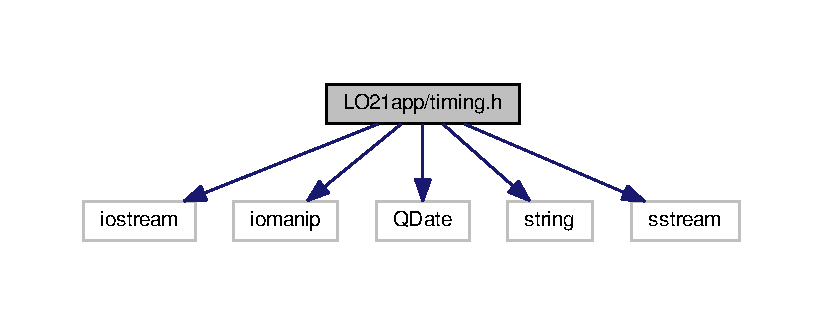
\includegraphics[width=350pt]{timing_8h__incl}
\end{center}
\end{figure}
This graph shows which files directly or indirectly include this file\+:\nopagebreak
\begin{figure}[H]
\begin{center}
\leavevmode
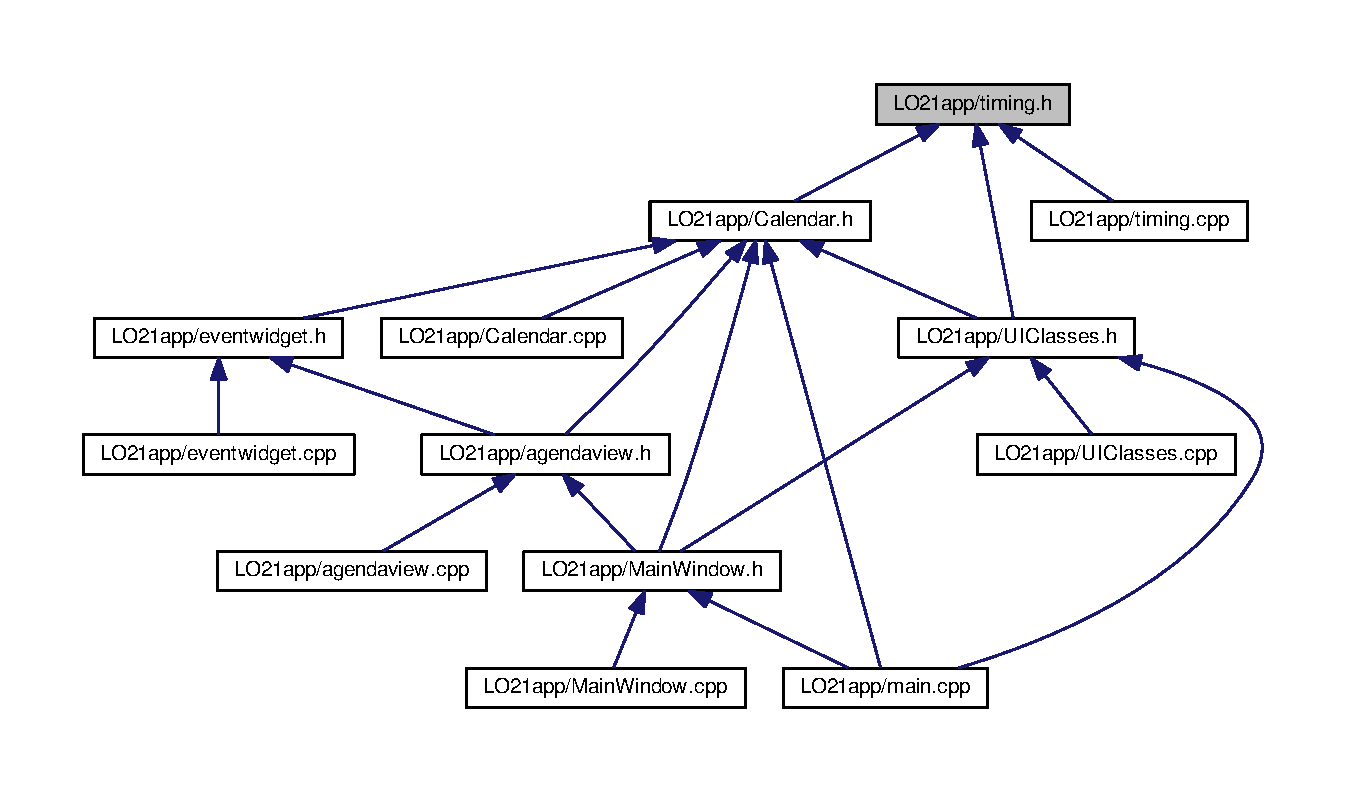
\includegraphics[width=350pt]{timing_8h__dep__incl}
\end{center}
\end{figure}
\subsection*{Classes}
\begin{DoxyCompactItemize}
\item 
class \hyperlink{class_t_i_m_e_1_1_time_exception}{T\+I\+M\+E\+::\+Time\+Exception}
\begin{DoxyCompactList}\small\item\em Classe permettant de g�rer les exceptions des classes du namespace \hyperlink{namespace_t_i_m_e}{T\+I\+M\+E}. \end{DoxyCompactList}\item 
class \hyperlink{class_t_i_m_e_1_1_date}{T\+I\+M\+E\+::\+Date}
\begin{DoxyCompactList}\small\item\em Classe permettant de manipuler des dates standards L\textquotesingle{}utilisation de cette classe n�cessite des dates valides au sens commun du terme. D�clenchement d\textquotesingle{}exception dans le cas contraire. \end{DoxyCompactList}\item 
class \hyperlink{class_t_i_m_e_1_1_duree}{T\+I\+M\+E\+::\+Duree}
\begin{DoxyCompactList}\small\item\em Classe permettant de manipuler des durees L\textquotesingle{}utilisation de cette classe n�cessite des dates valides au sens commun du terme. D�clenchement d\textquotesingle{}exception dans le cas contraire. \end{DoxyCompactList}\item 
class \hyperlink{class_t_i_m_e_1_1_horaire}{T\+I\+M\+E\+::\+Horaire}
\begin{DoxyCompactList}\small\item\em Classe permettant de manipuler des horaires L\textquotesingle{}utilisation de cette classe n�cessite des dates valides au sens commun du terme. D�clenchement d\textquotesingle{}exception dans le cas contraire. \end{DoxyCompactList}\item 
class \hyperlink{class_t_i_m_e_1_1_periode}{T\+I\+M\+E\+::\+Periode}
\begin{DoxyCompactList}\small\item\em Classe permettant de manipuler des periodes exprim�es en jours/mois/ann�es L\textquotesingle{}utilisation de cette classe n�cessite des dates valides au sens commun du terme. D�clenchement d\textquotesingle{}exception dans le cas contraire. \end{DoxyCompactList}\item 
class \hyperlink{class_t_i_m_e_1_1_intervalle}{T\+I\+M\+E\+::\+Intervalle}
\begin{DoxyCompactList}\small\item\em Classe permettant de manipuler des intervalles de dates L\textquotesingle{}utilisation de cette classe n�cessite des dates valides au sens commun du terme. D�clenchement d\textquotesingle{}exception dans le cas contraire. \end{DoxyCompactList}\end{DoxyCompactItemize}
\subsection*{Namespaces}
\begin{DoxyCompactItemize}
\item 
 \hyperlink{namespace_t_i_m_e}{T\+I\+M\+E}
\end{DoxyCompactItemize}
\subsection*{Functions}
\begin{DoxyCompactItemize}
\item 
std\+::ostream \& \hyperlink{timing_8h_ac43123d4d5341918e1cc3530dffc7430}{operator$<$$<$} (std\+::ostream \&, const \hyperlink{class_t_i_m_e_1_1_date}{T\+I\+M\+E\+::\+Date} \&)
\item 
std\+::ostream \& \hyperlink{timing_8h_ae1f6c691e21b37d44214d6d4b0ad86ab}{operator$<$$<$} (std\+::ostream \&f, const \hyperlink{class_t_i_m_e_1_1_duree}{T\+I\+M\+E\+::\+Duree} \&d)
\item 
std\+::ostream \& \hyperlink{timing_8h_ae97cb466b4f8db674e3f74d4eb9b42af}{operator$<$$<$} (std\+::ostream \&f, const \hyperlink{class_t_i_m_e_1_1_horaire}{T\+I\+M\+E\+::\+Horaire} \&h)
\item 
std\+::ostream \& \hyperlink{timing_8h_a7c8e3a6dcb0679a2ab5dfac4ced581df}{operator$<$$<$} (std\+::ostream \&f, const \hyperlink{class_t_i_m_e_1_1_periode}{T\+I\+M\+E\+::\+Periode} \&p)
\item 
std\+::ostream \& \hyperlink{timing_8h_aa5e474731ba5f5a00e8135c3610019ee}{operator$<$$<$} (std\+::ostream \&f, const \hyperlink{class_t_i_m_e_1_1_intervalle}{T\+I\+M\+E\+::\+Intervalle} \&p)
\item 
std\+::istream \& \hyperlink{timing_8h_a81d8973cae1411887907e7a60aa58a2c}{operator$>$$>$} (std\+::istream \&, \hyperlink{class_t_i_m_e_1_1_date}{T\+I\+M\+E\+::\+Date} \&)
\item 
std\+::istream \& \hyperlink{timing_8h_ae9c16fb88eebdd4a4cf7bfc49c9e6f31}{operator$>$$>$} (std\+::istream \&, \hyperlink{class_t_i_m_e_1_1_duree}{T\+I\+M\+E\+::\+Duree} \&)
\end{DoxyCompactItemize}


\subsection{Function Documentation}
\hypertarget{timing_8h_ac43123d4d5341918e1cc3530dffc7430}{}\index{timing.\+h@{timing.\+h}!operator$<$$<$@{operator$<$$<$}}
\index{operator$<$$<$@{operator$<$$<$}!timing.\+h@{timing.\+h}}
\subsubsection[{operator$<$$<$}]{\setlength{\rightskip}{0pt plus 5cm}std\+::ostream\& operator$<$$<$ (
\begin{DoxyParamCaption}
\item[{std\+::ostream \&}]{, }
\item[{const {\bf T\+I\+M\+E\+::\+Date} \&}]{}
\end{DoxyParamCaption}
)}\label{timing_8h_ac43123d4d5341918e1cc3530dffc7430}
\hypertarget{timing_8h_ae1f6c691e21b37d44214d6d4b0ad86ab}{}\index{timing.\+h@{timing.\+h}!operator$<$$<$@{operator$<$$<$}}
\index{operator$<$$<$@{operator$<$$<$}!timing.\+h@{timing.\+h}}
\subsubsection[{operator$<$$<$}]{\setlength{\rightskip}{0pt plus 5cm}std\+::ostream\& operator$<$$<$ (
\begin{DoxyParamCaption}
\item[{std\+::ostream \&}]{f, }
\item[{const {\bf T\+I\+M\+E\+::\+Duree} \&}]{d}
\end{DoxyParamCaption}
)}\label{timing_8h_ae1f6c691e21b37d44214d6d4b0ad86ab}
\hypertarget{timing_8h_ae97cb466b4f8db674e3f74d4eb9b42af}{}\index{timing.\+h@{timing.\+h}!operator$<$$<$@{operator$<$$<$}}
\index{operator$<$$<$@{operator$<$$<$}!timing.\+h@{timing.\+h}}
\subsubsection[{operator$<$$<$}]{\setlength{\rightskip}{0pt plus 5cm}std\+::ostream\& operator$<$$<$ (
\begin{DoxyParamCaption}
\item[{std\+::ostream \&}]{f, }
\item[{const {\bf T\+I\+M\+E\+::\+Horaire} \&}]{h}
\end{DoxyParamCaption}
)}\label{timing_8h_ae97cb466b4f8db674e3f74d4eb9b42af}
\hypertarget{timing_8h_a7c8e3a6dcb0679a2ab5dfac4ced581df}{}\index{timing.\+h@{timing.\+h}!operator$<$$<$@{operator$<$$<$}}
\index{operator$<$$<$@{operator$<$$<$}!timing.\+h@{timing.\+h}}
\subsubsection[{operator$<$$<$}]{\setlength{\rightskip}{0pt plus 5cm}std\+::ostream\& operator$<$$<$ (
\begin{DoxyParamCaption}
\item[{std\+::ostream \&}]{f, }
\item[{const {\bf T\+I\+M\+E\+::\+Periode} \&}]{p}
\end{DoxyParamCaption}
)}\label{timing_8h_a7c8e3a6dcb0679a2ab5dfac4ced581df}
\hypertarget{timing_8h_aa5e474731ba5f5a00e8135c3610019ee}{}\index{timing.\+h@{timing.\+h}!operator$<$$<$@{operator$<$$<$}}
\index{operator$<$$<$@{operator$<$$<$}!timing.\+h@{timing.\+h}}
\subsubsection[{operator$<$$<$}]{\setlength{\rightskip}{0pt plus 5cm}std\+::ostream\& operator$<$$<$ (
\begin{DoxyParamCaption}
\item[{std\+::ostream \&}]{f, }
\item[{const {\bf T\+I\+M\+E\+::\+Intervalle} \&}]{p}
\end{DoxyParamCaption}
)}\label{timing_8h_aa5e474731ba5f5a00e8135c3610019ee}
\hypertarget{timing_8h_a81d8973cae1411887907e7a60aa58a2c}{}\index{timing.\+h@{timing.\+h}!operator$>$$>$@{operator$>$$>$}}
\index{operator$>$$>$@{operator$>$$>$}!timing.\+h@{timing.\+h}}
\subsubsection[{operator$>$$>$}]{\setlength{\rightskip}{0pt plus 5cm}std\+::istream\& operator$>$$>$ (
\begin{DoxyParamCaption}
\item[{std\+::istream \&}]{, }
\item[{{\bf T\+I\+M\+E\+::\+Date} \&}]{}
\end{DoxyParamCaption}
)}\label{timing_8h_a81d8973cae1411887907e7a60aa58a2c}
\hypertarget{timing_8h_ae9c16fb88eebdd4a4cf7bfc49c9e6f31}{}\index{timing.\+h@{timing.\+h}!operator$>$$>$@{operator$>$$>$}}
\index{operator$>$$>$@{operator$>$$>$}!timing.\+h@{timing.\+h}}
\subsubsection[{operator$>$$>$}]{\setlength{\rightskip}{0pt plus 5cm}std\+::istream\& operator$>$$>$ (
\begin{DoxyParamCaption}
\item[{std\+::istream \&}]{, }
\item[{{\bf T\+I\+M\+E\+::\+Duree} \&}]{}
\end{DoxyParamCaption}
)}\label{timing_8h_ae9c16fb88eebdd4a4cf7bfc49c9e6f31}

\hypertarget{_u_i_classes_8cpp}{}\section{L\+O21app/\+U\+I\+Classes.cpp File Reference}
\label{_u_i_classes_8cpp}\index{L\+O21app/\+U\+I\+Classes.\+cpp@{L\+O21app/\+U\+I\+Classes.\+cpp}}
{\ttfamily \#include \char`\"{}U\+I\+Classes.\+h\char`\"{}}\\*
Include dependency graph for U\+I\+Classes.\+cpp\+:\nopagebreak
\begin{figure}[H]
\begin{center}
\leavevmode
\includegraphics[width=350pt]{_u_i_classes_8cpp__incl}
\end{center}
\end{figure}

\hypertarget{_u_i_classes_8h}{}\section{L\+O21app/\+U\+I\+Classes.h File Reference}
\label{_u_i_classes_8h}\index{L\+O21app/\+U\+I\+Classes.\+h@{L\+O21app/\+U\+I\+Classes.\+h}}
{\ttfamily \#include $<$Q\+Standard\+Item\+Model$>$}\\*
{\ttfamily \#include $<$Q\+Standard\+Item$>$}\\*
{\ttfamily \#include $<$Q\+Line\+Edit$>$}\\*
{\ttfamily \#include $<$typeinfo$>$}\\*
{\ttfamily \#include $<$Q\+Form\+Layout$>$}\\*
{\ttfamily \#include $<$Q\+Push\+Button$>$}\\*
{\ttfamily \#include $<$Q\+Calendar\+Widget$>$}\\*
{\ttfamily \#include $<$Q\+Signal\+Mapper$>$}\\*
{\ttfamily \#include \char`\"{}Calendar.\+h\char`\"{}}\\*
{\ttfamily \#include \char`\"{}timing.\+h\char`\"{}}\\*
{\ttfamily \#include $<$Q\+Check\+Box$>$}\\*
{\ttfamily \#include $<$Q\+Spin\+Box$>$}\\*
{\ttfamily \#include $<$Q\+Date$>$}\\*
{\ttfamily \#include $<$Q\+List\+Widget$>$}\\*
{\ttfamily \#include $<$Q\+List\+Widget\+Item$>$}\\*
{\ttfamily \#include $<$Q\+Label$>$}\\*
{\ttfamily \#include $<$Q\+Combo\+Box$>$}\\*
{\ttfamily \#include $<$Q\+Dialog$>$}\\*
{\ttfamily \#include $<$Q\+Message\+Box$>$}\\*
{\ttfamily \#include $<$Q\+File\+Dialog$>$}\\*
{\ttfamily \#include $<$Q\+Icon$>$}\\*
Include dependency graph for U\+I\+Classes.\+h\+:\nopagebreak
\begin{figure}[H]
\begin{center}
\leavevmode
\includegraphics[width=350pt]{_u_i_classes_8h__incl}
\end{center}
\end{figure}
This graph shows which files directly or indirectly include this file\+:\nopagebreak
\begin{figure}[H]
\begin{center}
\leavevmode
\includegraphics[width=350pt]{_u_i_classes_8h__dep__incl}
\end{center}
\end{figure}
\subsection*{Classes}
\begin{DoxyCompactItemize}
\item 
class \hyperlink{class_tree_view_model}{Tree\+View\+Model}
\begin{DoxyCompactList}\small\item\em Gestionnaire singloton du modèle du Tree\+View~\newline
 \end{DoxyCompactList}\item 
class \hyperlink{class_editeur}{Editeur}
\begin{DoxyCompactList}\small\item\em Classe abstraite pour le widget d\textquotesingle{}édition (partie droite de l\textquotesingle{}onglet d\textquotesingle{}édition) \end{DoxyCompactList}\item 
class \hyperlink{class_editeur_projet}{Editeur\+Projet}
\begin{DoxyCompactList}\small\item\em Classe pour l\textquotesingle{}\hyperlink{class_editeur}{Editeur} de projet. \end{DoxyCompactList}\item 
class \hyperlink{class_editeur_tache}{Editeur\+Tache}
\begin{DoxyCompactList}\small\item\em Classe abstraite pour l\textquotesingle{}\hyperlink{class_editeur}{Editeur} de taches. \end{DoxyCompactList}\item 
class \hyperlink{class_editeur_t_u}{Editeur\+T\+U}
\begin{DoxyCompactList}\small\item\em \hyperlink{class_editeur_tache}{Editeur\+Tache} de taches unitaires. \end{DoxyCompactList}\item 
class \hyperlink{class_editeur_t_c}{Editeur\+T\+C}
\begin{DoxyCompactList}\small\item\em \hyperlink{class_editeur_tache}{Editeur\+Tache} de taches composite. \end{DoxyCompactList}\item 
class \hyperlink{class_editeur_precedence}{Editeur\+Precedence}
\begin{DoxyCompactList}\small\item\em \hyperlink{class_editeur}{Editeur} des précédences de la tache appelante. \end{DoxyCompactList}\item 
class \hyperlink{class_programmation_tache}{Programmation\+Tache}
\begin{DoxyCompactList}\small\item\em Programme la tache sélectionnée dans le tree view. \end{DoxyCompactList}\item 
class \hyperlink{class_programmation_activite}{Programmation\+Activite}
\begin{DoxyCompactList}\small\item\em Dialogue de programmation d\textquotesingle{}une activité \end{DoxyCompactList}\end{DoxyCompactItemize}

%--- End generated contents ---

% Index
\backmatter
\newpage
\phantomsection
\clearemptydoublepage
\addcontentsline{toc}{chapter}{Index}
\printindex

\end{document}
